% Template for PLoS
% Version 3.6 Aug 2022
%
% % % % % % % % % % % % % % % % % % % % % %
%
% -- IMPORTANT NOTE
%
% This template contains comments intended 
% to minimize problems and delays during our production 
% process. Please follow the template instructions
% whenever possible.
%
% % % % % % % % % % % % % % % % % % % % % % % 
%
% Once your paper is accepted for publication, 
% PLEASE REMOVE ALL TRACKED CHANGES in this file 
% and leave only the final text of your manuscript. 
% PLOS recommends the use of latexdiff to track changes during review, as this will help to maintain a clean tex file.
% Visit https://www.ctan.org/pkg/latexdiff?lang=en for info or contact us at latex@plos.org.
%
%
% There are no restrictions on package use within the LaTeX files except that no packages listed in the template may be deleted.
%
% Please do not include colors or graphics in the text.
%
% The manuscript LaTeX source should be contained within a single file (do not use \input, \externaldocument, or similar commands).
%
% % % % % % % % % % % % % % % % % % % % % % %
%
% -- FIGURES AND TABLES
%
% Please include tables/figure captions directly after the paragraph where they are first cited in the text.
%
% DO NOT INCLUDE GRAPHICS IN YOUR MANUSCRIPT
% - Figures should be uploaded separately from your manuscript file. 
% - Figures generated using LaTeX should be extracted and removed from the PDF before submission. 
% - Figures containing multiple panels/subfigures must be combined into one image file before submission.
% For figure citations, please use "Fig" instead of "Figure".
% See http://journals.plos.org/plosone/s/figures for PLOS figure guidelines.
%
% Tables should be cell-based and may not contain:
% - spacing/line breaks within cells to alter layout or alignment
% - do not nest tabular environments (no tabular environments within tabular environments)
% - no graphics or colored text (cell background color/shading OK)
% See http://journals.plos.org/plosone/s/tables for table guidelines.
%
% For tables that exceed the width of the text column, use the adjustwidth environment as illustrated in the example table in text below.
%
% % % % % % % % % % % % % % % % % % % % % % % %
%
% -- EQUATIONS, MATH SYMBOLS, SUBSCRIPTS, AND SUPERSCRIPTS
%
% IMPORTANT
% Below are a few tips to help format your equations and other special characters according to our specifications. For more tips to help reduce the possibility of formatting errors during conversion, please see our LaTeX guidelines at http://journals.plos.org/plosone/s/latex
%
% For inline equations, please be sure to include all portions of an equation in the math environment. For example, x$^2$ is incorrect; this should be formatted as $x^2$ (or $\mathrm{x}^2$ if the romanized font is desired).
%
% Do not include text that is not math in the math environment. For example, CO2 should be written as CO\textsubscript{2} instead of CO$_2$.
%
% Please add line breaks to long display equations when possible in order to fit size of the column. 
%
% For inline equations, please do not include punctuation (commas, etc) within the math environment unless this is part of the equation.
%
% When adding superscript or subscripts outside of brackets/braces, please group using {}. For example, change "[U(D,E,\gamma)]^2" to "{[U(D,E,\gamma)]}^2". 
%
% Do not use \cal for caligraphic font. Instead, use \mathcal{}
%
% % % % % % % % % % % % % % % % % % % % % % % % 
%
% Please contact latex@plos.org with any questions.
%
% % % % % % % % % % % % % % % % % % % % % % % %

\documentclass[10pt,letterpaper]{article}
\usepackage[top=0.85in,left=2.75in,footskip=0.75in]{geometry}

\usepackage[utf8]{inputenc}

% amsmath and amssymb packages, useful for mathematical formulas and symbols
\usepackage{amsmath,amssymb}

% Use adjustwidth environment to exceed column width (see example table in text)
\usepackage{changepage}

% textcomp package and marvosym package for additional characters
\usepackage{textcomp,marvosym}

% cite package, to clean up citations in the main text. Do not remove.
\usepackage{cite}

\usepackage{listings}
\usepackage[T1]{fontenc}

% Use nameref to cite supporting information files (see Supporting Information section for more info)
\usepackage{nameref,hyperref}

% line numbers
\usepackage[right]{lineno}

% ligatures disabled
\usepackage[nopatch=eqnum]{microtype}
\DisableLigatures[f]{encoding = *, family = * }

% color can be used to apply background shading to table cells only
\usepackage[table]{xcolor}

% array package and thick rules for tables
\usepackage{array}

% package for drawing trees
\usepackage{forest}

\usepackage{float}
\usepackage{subcaption}
\usepackage{dirtytalk}

% create "+" rule type for thick vertical lines
\newcolumntype{+}{!{\vrule width 2pt}}

% create \thickcline for thick horizontal lines of variable length
\newlength\savedwidth
\newcommand\thickcline[1]{%
 \noalign{\global\savedwidth\arrayrulewidth\global\arrayrulewidth 2pt}%
 \cline{#1}%
 \noalign{\vskip\arrayrulewidth}%
 \noalign{\global\arrayrulewidth\savedwidth}%
}

% \thickhline command for thick horizontal lines that span the table
\newcommand\thickhline{\noalign{\global\savedwidth\arrayrulewidth\global\arrayrulewidth 2pt}%
\hline
\noalign{\global\arrayrulewidth\savedwidth}}


% Remove comment for double spacing
%\usepackage{setspace} 
%\doublespacing

% Text layout
\raggedright
\setlength{\parindent}{0.5cm}
\textwidth 5.25in 
\textheight 8.75in

% Bold the 'Figure #' in the caption and separate it from the title/caption with a period
% Captions will be left justified
\usepackage[aboveskip=1pt,labelfont=bf,labelsep=period,justification=raggedright,singlelinecheck=off]{caption}
\renewcommand{\figurename}{Fig}

% Use the PLoS provided BiBTeX style
\bibliographystyle{plos2015}

% Remove brackets from numbering in List of References
\makeatletter
\renewcommand{\@biblabel}[1]{\quad#1.}
\makeatother

\lstset{literate={~} {$\sim$}{1}}
                 
% Header and Footer with logo
\usepackage{lastpage,fancyhdr,graphicx}
\usepackage{epstopdf}
%\pagestyle{myheadings}
\pagestyle{fancy}
\fancyhf{}
%\setlength{\headheight}{27.023pt}
%\lhead{\includegraphics[width=2.0in]{PLOS-submission.eps}}
\rfoot{\thepage/\pageref{LastPage}}
\renewcommand{\headrulewidth}{0pt}
\renewcommand{\footrule}{\hrule height 2pt \vspace{2mm}}
\fancyheadoffset[L]{2.25in}
\fancyfootoffset[L]{2.25in}
\lfoot{\today}

%% Include all macros below

\newcommand{\Pro}[1]{P\left(#1\right)} 
\newcommand{\ProT}[1]{P_\theta\left(#1\right)} 
\newcommand{\Ex}[1]{\textbf{E}\left[#1\right]} 
\newcommand{\Var}[1]{\mathrm{Var}\left(#1\right)} 

%% END MACROS SECTION

\usepackage{booktabs}

\begin{document}
\vspace*{0.2in}

% Title must be 250 characters or less.
\begin{flushleft}
{\Large
\textbf\newline{Tractable time tree distributions} % Please use "sentence case" for title and headings (capitalize only the first word in a title (or heading), the first word in a subtitle (or subheading), and any proper nouns).
}
\newline
% Insert author names, affiliations and corresponding author email (do not include titles, positions, or degrees).
\\
Tobia Ochsner\textsuperscript{1, 2},
Jonathan Klawitter\textsuperscript{1},
Alexei J. Drummond\textsuperscript{1}*,
\\
\bigskip
\textbf{1} University of Auckland, Auckland, Aotearoa/New Zealand
\\
\textbf{2} ETH Zurich, Basel, Switzerland
\\
\bigskip

% Use the asterisk to denote corresponding authorship and provide email address in note below.
* a.drummond@auckland.ac.nz

\end{flushleft}
% Please keep the abstract below 300 words
\section*{Abstract}
In Bayesian phylogenetics, Markov Chain Monte Carlo (MCMC) methods generate samples of time trees to capture the posterior distribution of the phylogenetic tree. We explore novel approaches to fit distributions on these time trees samples. In particular, we extend the family of Conditional Clade Distributions (CCD) to model the tree topology and branch lengths simultaneously. Our distributions are designed to capture both central tendencies and dependencies within this high-dimensional and non-Euclidean space. They facilitate a straightforward reconstruction of a summary tree and manage to capture the tails of the time tree distribution. This property extends their utility beyond the robust reconstruction of a single summary tree, enabling more sophisticated downstream analyses like exploring credible regions or evaluating alternative evolutionary hypotheses.


% Please keep the Author Summary between 150 and 200 words
% Use first person. PLOS ONE authors please skip this step. 
% Author Summary not valid for PLOS ONE submissions.  
\section*{Author summary}

% TODO

\linenumbers

% Use "Eq" instead of "Equation" for equation citations.
\section*{Introduction}

Markov Chain Monte Carlo (MCMC) methods have become a cornerstone of Bayesian phylogenetics. Given a set of aligned molecular sequences and an evolutionary model (consisting of a tree model, a molecular clock model, a substitution model, and prior distributions on parameters), MCMC algorithms like Beast 2 \cite{beast2}, RevBayes \cite{revbayes} or MrBayes \cite{mrbayes} generate a set of phylogenetic trees sampled from the posterior distribution. This posterior sample usually consists of thousands of trees and contains a wealth of information about the evolutionary relationships encoded in the provided sequences.

For simple continuous or indicator parameters of the phylogenetic model (like substitution or clock rates), analyzing the marginal distributions of the posterior sample is relatively straightforward. Tools like Tracer \cite{tracer} provide readily available summaries and visualizations of these marginal distributions.

The space of phylogenetic trees presents a significantly greater challenge. The sheer number of possible rooted trees explodes super-exponentially with increasing taxa, making it highly unlikely that the MCMC samples contain the true tree topology \cite{ccd}. The \emph{curse of dimensionality} \cite{curse,curse2} diminishes the effectiveness of common sample-based statistical methods, particularly distance-based approaches. As demonstrated in the Supplementary Information, MCMC samples can exhibit strikingly similar pairwise distances, contradicting the expectation that regions of higher probability density should yield samples with closer proximity. Furthermore, the space of possible divergence times is non-Euclidean, as the times are inherently constrained by the topology \cite{steelsemple,wald,tauspace,tropical,bhv}. These challenges make it difficult to directly analyze the posterior sample of trees and branch lengths. One strategy to extract meaningful information from the sample involves dedicated post-processing techniques. The raw sample is distilled into representations that enable a more meaningful analysis and interpretation.

A common approach is to infer a point estimate, a single \say{best} tree that summarizes the posterior sample \cite{treesinforest}. Several heuristics have been developed for this purpose, including DensiTree visualizations \cite{densitree}, Maximum Clade Credibility (MCC) trees, Hipster \cite{hipstr}, and the Maximum A Posteriori tree based on Conditional Clade Distributions (CCD) \cite{ccd,ccdlarget}. These methods often focus primarily on recovering a likely tree topology. Determining branch lengths is treated as an afterthought, potentially overlooking important information about evolutionary timescales.

Another class of algorithms simultaneously considers tree topology and branch lengths by embedding trees in a particular metric space. Examples include the Billera-Holmes-Vogtmann (BHV) space \cite{bhv}, the Wald space \cite{wald}, the $t$ and $\tau$ space \cite{tauspace}, the palm tree space \cite{tropical}, the RNNI space \cite{rnnispace}, and the recently developed Wald space \cite{wald}. Within these spaces, a natural approach to obtain a point estimate is to calculate the Fréchet mean of the posterior tree sample \cite{frechetmeanvar}. However, these spaces often suffer from limitations such as the \emph{sticky mean problem} (where the mean tree is almost independent of the actual tree samples) \cite{sticky}, high computational complexity associated with distance calculations, and the inherent difficulties of performing statistical inference in complex geometric spaces \cite{riemanngaussian}.

While obtaining a point estimate from the posterior sample is crucial, it is important to recognize that the MCMC sample contains information about the entire posterior distribution. Tractable tree distributions \cite{ccd} try to capture the posterior distribution using a well-defined approximate distribution. This provides an elegant framework for testing alternative evolutionary hypotheses, determining whether a specific tree falls within a credible region, calculating statistics like information content \cite{informationcontent}, and analyzing dependencies between different parts of the tree (e.g., relationships between branch lengths and topological features). Existing methods that estimate distributions on the posterior sample for rooted trees focus on modeling tree topologies \cite{ccd,ccdlarget}, ignoring time information entirely. The family of Bayesian subsplit networks \cite{subsplit} has been extended to model branch lengths in multiple ways \cite{subsplitnf,subsplitbranchlengths,artree}. However, Bayesian subsplit methods focus on direct variational inference, rather than posterior sample summarization.

Here, we address the challenge of inferring tractable distributions on time trees, encompassing both topology and branch lengths. We compare different methods and tree embeddings, and demonstrate that the described methods exhibit significant differences in terms of capturing central tendencies and the tails of the distribution. Finally, we introduce a software package that enables researchers to fit and analyze these distributions, facilitating more nuanced insight into phylogenetic uncertainty. This tool allows for a more complete utilization of the information within the posterior tree sample, moving beyond simple point estimates.

\section*{Materials and methods}

In this section, we introduce the concept of tractable tree distributions on time trees and discuss desirable properties of such distributions. We then introduce a family of distributions satisfying these properties and show how to perform common operations such as parameter estimation and obtaining a point estimate. Finally, we outline the procedure used to assess and compare the distributions on both synthetic and real datasets.

\subsection*{Tractable tree distributions}

Berling et al. \cite{ccd} introduced \emph{tractable tree distributions} as a set of properties of a distribution on tree topologies. A distribution is tractable if a range of operations can be performed efficiently in practice. We apply the same concept to distributions on \emph{time trees}.

Tractable time tree distributions are used as a tool to analyze a posterior tree sample. Therefore, we should be able to efficiently infer its parameters based on that tree sample. In order to compare different tree hypotheses, we need to evaluate the probability density of any time tree under the model. Another important operation is sampling, as it enables to test if a tree is in the 95\% credible region and to inspect the dependencies of different node heights. Lastly, a tractable time tree distribution should provide us with a \emph{summary tree}, for instance by retrieving the highest-probability or expected tree.

\subsection*{Mathematical framework}

A \emph{time tree} $(T, \{H_v\}_{v \in V})$ for a set of taxa $X$ and root $R$ consists of an undirected tree $T = (V, E)$ and a set of random variables $\{H_v\}_{v \in V} \in \mathbb{R}^+$ denoting the vertex heights (the divergence times). The following properties have to be satisfied:

\begin{enumerate}
	\item $(V, E)$ describes a fully connected tree.
	\item The root $R \in V$ has degree $2$. The taxa $X \subset V$ have degree $1$. All other vertices are \emph{internal} vertices and have degree $3$.
	\item We only consider contemporary sampling of the taxa: $H_x = 0$ for all taxa $x$.
	\item Each edge $e$ in $E$ consists of a parent $p$ and child $c$ such that the parent is closer to the root. The heights must describe a valid tree and evolution runs backward in time: $H_c < H_p$ for all edges $(p, c)$ in $E$.
\end{enumerate}

The probability of a time tree can be factorized into the probability of its topology $T$ and the probability of the vertex heights $\{H_v\}_{v \in V}$ given the topology:

$$
\Pro{T, \{H_v\}_{v \in V}} = \Pro{T} \Pro{\{H_v\}_{v \in V} | T}.
$$

To model $\Pro{T}$, we use the conditional clade distributions \emph{CCD0} and \emph{CCD1} \cite{ccd,ccdlarget}. They exhibit the desired properties and have shown to work well in practice \cite{ccd,ccd0expansion,hipstr}. Thus, we focus on modelling the conditional probability $\Pro{\{H_v\}_{v \in V} | T}$. It is crucial to note that we do not restrict ourselves to a single topology $T$---we simply model $\Pro{\{H_v\}_{v \in V} | T}$ as a function of the topology $T$.

\subsection*{Credible regions}

A key tool in our analysis is the \emph{smallest $\gamma$-credible region} of the tree posterior. This region, defined as the minimum set of time trees with a combined probability mass of $\gamma$, provides a straightforward way to assess the compatibility of a tree with the posterior. It allows, for instance, to determine if a time tree obtained with a completely different methodology is in the smallest 95\%-credible region (a random posterior tree has a 95\% probability of being in the 95\%-credible region). There is a surprisingly simple way to assess if a given time tree is within the smallest $\gamma$-credible region of a distribution: We generate a large number of samples from the distribution and rank the model probabilities of the generated trees. If the model probability of the given tree ranks within the top $\gamma$\% of the sampled tree probabilities, it is in the smallest $\gamma$-credible region. This approach works because every point inside the smallest credible region has a probability density at least as large as any point outside the region.

\subsection*{Clade parameterisation}

There are several main challenges when designing a distribution on the heights.

First, $P\left(\{H_v\}_{v \in V} | T\right)$ is a function of the topology $T$. However, we cannot assume that every possible topology is found in the MCMC sample. Hence, $P\left(\{H_v\}_{v \in V} | T\right)$ needs to be defined even for unknown topologies. Moreover, as the number of possible topologies can be extremly large, we have to share parameters amongst different topologies. In order to overcome this challenge, we employ the same strategy as the CCD0 model \cite{ccd}: instead of having random variables correspond to vertices of a topology, they correspond to clades.

$$
\Pro{\{H_v\}_{v \in V} | T} = \Pro{\{H_c\}_{c \in C(T)} | T},
$$

where $C(T)$ is the set of clades in topology $T$. A clade is a subset of taxa that share a common ancestor. While every vertex corresponds to exactly one clade, modeling random variables on a clade-level allows to share parameters amongst different topologies that have common clades. We call a clade \emph{non-trivial} if it is neither a singleton nor the root clade. In the following, we exclude the singleton clades corresponding to the taxa from $C(T)$, as $H_c$ equals $0$ for all singleton clades and does not need to be modelled. 

Another difficulty is the fact that every topology enforces a different set of constraints on the heights. We expect $P\left(\{H_c\}_{c \in C(T)} | T\right)$ to vanish for heights invalid under the topology. We solve this by introducing the concept of a \emph{clade embedding}. Given a topology $T$, a clade embedding $f_T$ induces a bijection from the heights into another set of random variables in the \emph{embedding space}:

$$
f_T: \{H_c\}_{c \in C(T)} \mapsto \{Z_c\}_{c \in C(T)}.
$$

The embedding can be designed such that the $Z_c$ have nice constraints independent of the topology (for instance, $Z_c \in \mathbb{R}$ or $Z_c \in [0, 1]$). Equipped with an embedding, we can define a probability distribution on $\{Z_c\}_{c \in C(T)}$ and the corresponding pulled-back probability distribution on $\{H_c\}_{c \in C(T)}$:

$$
P\left(\{H_c\}_{c \in C(T)} | T\right) = P\left(\{Z_c\}_{c \in C(T)} | T\right) \left| \det{\left(J_{f_t^{-1}}(\{Z_c\}_{c \in C(T)})\right)} \right|,
$$

where $J_{f_t^{-1}}(\{Z_c\}_{c \in C(T)})$ is the Jacobian of the inverse of the embedding.

We can choose commonly used probability distributions in the embedding space. In combination with a tractable embedding and inverse embedding, this leads to a probability distribution that is both tractable and respects the inherent constraints on the vertex heights. In order to get the probability of a set of heights under a topology, we first transform the set of heights into the embedding space. Then, we can use the pulled-back probability distribution to calculate the probability. If we want to sample from the distribution, we can sample from the embedding space and transform the samples back into the original height space.

There is another challenge that arises when designing a distribution on the heights. Dependencies between node heights are fundamentally tied to the height constraints and the restriction to contemporary sampling. However, other factors can influence branch length dependencies as well. For instance, a root height calibration prior can cause an anti-correlation between the pendant branch lengths and external branch lengths. The chosen embedding method can also affect these dependencies, possibly decreasing the correlation of the embedded random variables.

In the following sections, we introduce three clade embeddings equipped with different strategies for assigning probabilities in the embedding space (see figures \ref{fig:example1} and \ref{fig:example2} for examples). Our general approach is to find the best approximation of the marginal time tree posterior distribution of the MCMC model. Thus, biological interpretation of the designed distributions is not a primary goal. Instead, we focus on a wide range of embeddings and distributions that fulfill the properties of tractable time tree distributions and then compare their fit with the MCMC posterior distribution on a variety of real-world and simulated datasets.

\begin{figure}[H]
    \caption{This example shows the same time tree embedded into the different embedding spaces. We assign a value to every non-singleton clade. The second column (Absolute heights) contains the absolute vertex height. The third column (Last divergence) denotes the time since the last divergence for the root vertex and the length of the branch leading to a vertex for the internal vertices. The third embedding (Shorter branch) denotes the length of the branch leading to the older child. The last column (Shorter branch) represents the total tree height for the root clade and the ratio of the internal vertices to their parents.}
	
	\hspace{10pt}

	\centering
    \begin{forest}
        [ABCDE
            [ABC, l=20mm
                [A, l=30mm]
                [AB, l=20mm
                       [B, l=10mm]
                       [C, l=10mm]
                ]
            ]
            [DE, l=30mm
                [D, l=20mm]
                [E, l=20mm]	
            ]
        ]
    \end{forest}
    
    \hspace{10pt}
    
    \begin{tabular}{@{}lcccc@{}}
        \toprule
          Clade & Absolute heights & Last divergence & Shorter branch & Height ratio \\
        \midrule
        ABCDE & 50 & 10 & 20 & 50 \\
            ABC & 30 & 20 & 20 & 0.6 \\
            AB & 10 & 20 & 10 & 0.33 \\
            DE & 20 & 30 & 20 & 0.4 \\
        \bottomrule
    \end{tabular}

	\label{fig:example1}
\end{figure}

\begin{figure}[H]
	\caption{A second example.}

	\hspace{10pt}

    \centering
    \begin{forest}
        [ABCDE
            [ABCD, l=10mm
                [AB, l=30mm
                       [A, l=10mm]
                       [B, l=10mm]
                ]
                [CD, l=20mm
                       [C, l=20mm]
                       [D, l=20mm]
                ]
            ]
            [E, l=50mm]
        ]
    \end{forest}
    
    \hspace{10pt}
    
    \begin{tabular}{@{}lcccc@{}}
        \toprule
          Clade & Absolute heights & Last divergence & Shorter branch & Height ratio \\
        \midrule
            ABCDE & 50 & 10 & 10 & 50 \\
            ABCD & 40 & 10 & 20 & 0.8 \\
            AB & 10 & 30 & 10 & 0.25 \\
            CD & 20 & 20 & 20 & 0.5 \\
        \bottomrule
    \end{tabular}
    
    \label{fig:example2}
\end{figure}

\subsection*{Last divergence embedding}

Under the birth death model, internal branch lengths are assumed to be independent realizations of a stochastic evolutionary process. In contrast, pendant branch lengths are primarily influenced by the time of sampling. We propose to model internal branch lengths using independent distributions, while separatly accounting for the time between sampling and the last divergence event. This approach aligns with theoretical findings suggesting that internal and pendant branch lengths follow notably different distributions \cite{birthdeathdistribution,birthdeathdistributionstadler}.

Specifically, we consider the branch length leading to a vertex $v$ corresponding to a non-trivial clade $c$:

$$
Z_c = H_{p_v} - H_v.
$$

Furthermore, we consider the time between the present and the last divergence event and assign it to the random variable corresponding to the root clade $X$:

$$
Z_X = \min_{c \in C(T)}{H_c}.
$$

This embedding allows to choose arbitrary positive $Z_c$ while always producing a valid tree. Thus, we propose to use either independent lognormal, independent gamma, or independent Weibull distributions:

$$
P(\{Z_c\}_{c \in C(T)}) = \begin{cases}
	\prod_{c \in C(T)}{LogNormal(Z_c; \mu_c, \sigma_c)}, \\
	\prod_{c \in C(T)}{Gamma(Z_c; \alpha_c, \beta_c)}, \\
	\prod_{c \in C(T)}{Weibull(Z_c; k_c, \lambda_c)}.
\end{cases}
$$

Different models for divergence suggest different distributions on the branch lengths \cite{venditti2010phylogenies}. For instance, a constant rate of divergence results in an exponential distribution, which is a special case of both the gamma and the weibull distribution. If the rate of divergence changes with the amount of time since the last divergence, the resulting distribution will be closer to a Weibull distribution.

\subsection*{Shorter branch embedding}

We introduce an alternative embedding that directly utilizes absolute branch lengths. For a clade $c$ corresponding to vertex $v$, we define $Z_c$ as the branch length leading to the older child of $v$.

$$
Z_c = H_v - \max{\left(H_{a_v}, H_{b_v}\right)},
$$

where $a_v$ and $b_v$ represent the two child vertices of $v$. This parameterisation ensures that any set of positive $Z_c$, given a topology, results in a valid contemporary sampled time tree. To assign probabilities to these branch lengths, we consider same the three probabilistic models:

$$
P(\{Z_c\}_{c \in C(T)}) = \begin{cases}
	\prod_{c \in C(T)}{LogNormal(Z_c; \mu_c, \sigma_c)}, \\
	\prod_{c \in C(T)}{Gamma(Z_c; \alpha_c, \beta_c)}, \\
	\prod_{c \in C(T)}{Weibull(Z_c; k_c, \lambda_c)}.
\end{cases}
$$

\subsection*{Height ratio embedding}

Inspired by TreeFlow \cite{treeflow}, we introduce the height ratio embedding to capture the relative temporal structure of the vertices in time trees. For any non-trivial clade $c$ correspoding to vertex $v$, we define $Z_c$ as the ratio of the height of $v$ to the height of its parent $p_v$.

$$
Z_c = \frac{H_v}{H_{p_v}}.
$$

In addition to the relative positions of the vertices, we model the overall height of the time tree using the random variable corresponding to the root clade $X$:

$$
Z_X = H_R.
$$

Consequently, $Z_X$ takes values in $\mathbb{R}^+$. For any non-trivial clade $c$, $Z_c$ is constrained to the interval $[0, 1]$. The primary advantage of the height ratio embedding lies in its ability to mitigate the effects of dependencies introduced by contemporary sampling and potential calibration priors.

We model the ratios and the tree height independently. For the height ratios, we consider the following probability distributions:

$$
P(\{Z_c\}_{c \in C(T) \setminus X}) = \begin{cases}
	\prod_{c \in C(T) \setminus X}{Beta(Z_c; \alpha_c, \beta_c)}, \\
	\prod_{c \in C(T) \setminus X}{LogitNormal(Z_c; \mu_c, \sigma_c)}.
\end{cases}
$$

We further experimented with a generalized Dirichlet distribution, parameterized by a single parameter for each non-trivial clade. It is a special case of the independent beta distributions, defined such that the marginal distribution of any path from the root vertex to a leaf follows a Dirichlet distribution. However, it did not perform nearly as well as the other distributions and parameter estimation was not as straightforward, leading to an exclusion from the comparison.

We model the overall tree height with a lognormal distribution:

$$
P(Z_X) = \text{LogNormal}(Z_X; \mu_X, \sigma_X).
$$

\subsection*{Operations on tractable time tree distributions}

We use the maximum likelihood estimator to estimate the parameters for each embedding and the corresponding distributions. The stated independence assumptions significantly simplify this process, reducing it to the maximum likelihood estimation of basic univariate continuous distributions. For the lognormal and logitnormal distribution, the maximum likelihood estimators exhibit well-known closed form solutions. We apply Newton's method for the gamma, beta and weibull distributions. A fundamental assumption of the maximum likelihood estimators is that the samples are independent. To meet this assumption for the MCMC time trees, we estimate the effective sample size (tree ESS) and only use a corresponding subsample to fit the distribution. The ESS is estimated using a procedure described in the Supporting Information.

In order to calculate the probability for a given time tree, we first transform the set of heights into the embedding space. Then, we can use the pulled-back probability distribution to calculate the probability. Sampling from the distribution is achieved by drawing samples from the embedding space and mapping them back to the original height space using the inverse transformation. Another important operation is constructing a point estimate based on a fitted tractable time tree distribution. One natural choice is the highest probability tree, as it is done for the CCD distributions \cite{ccd}. For models based on gamma, beta or weibull distributions, this can lead to a tree with branch lengths of $0$. Hence, we use the expected vertex heights as a point estimate.

To determine if a tree is in the smallest $\gamma$-credible region of the approximated posterior distribution, we first sample from the distribution and rank the model probabilities of the generated time trees. A given tree is in the smallest $\gamma$-credible region if its model probability ranks within the top $\gamma$\% of the sampled tree probabilities.

A final operation that becomes tractable for the given embeddings is the calculation of the (differential) entropy of the distribution:

\begin{equation*}
	\begin{split}
		h(\{H_v\}_{v \in V}) = &h(\{Z_c\}_{c \in C(T)}) \\
		& + \int P(\{Z_c\}_{c \in C(T)}) \log \left| \det{\left(J_{f_t^{-1}}(\{Z_c\}_{c \in C(T)})\right)} \right| d \{Z_c\}_{c \in C(T)}.
	\end{split}
\end{equation*}

\subsection*{Validation}

We use two complementary approaches to evaluate the quality of our proposed tractable time tree distributions: \emph{model comparison} and \emph{goodness-of-fit (GoF) testing}. We perform a train-validation split of the decorrelated subsample of the posterior time trees. The first 75\% of the posterior samples is used as the training set for parameter estimation, while the remaining 25\% is used as the validation set.

Given a posterior set of time trees, we calculate the data likelihood to compare the relative performance of our distributions on that set. Since all our models have the same number of parameters, we do not have to use a metric like the Akaike Information Criterion (AIC) to balance the likelihood with the parameter count. While the likelihood allows us to rank different models, it does not determine if any model accurately reflects the posterior distribution.

Hence, we also perform a visual goodness-of-fit test to assess how well our tractable tree distributions capture the posterior distribution. The test is based on the credible regions of the fitted distributions and compares them to the MCMC posterior samples. Specifically, we count the number of MCMC trees in the smallest $\gamma$-credible regions of the fitted distribution for different values of $\gamma$. If the approximation is successful, we expect $\gamma$\% of the MCMC trees to be in the smallest $\gamma$-credible region. Plotting the fraction for every credible region should thus result in a straight line. We use the \emph{Cramér-von Mises} criterion \cite{cramarvonmises} to quantify the deviation from the $x=y$ line by calculating the sum of the squared differences between the observed and expected fraction of trees in the smallest $\gamma$-credible region. The smaller the value, the better the fit.

There is a close connection to the \emph{rank-uniformity plots} used in Bayesian model validation (first introduced by \cite{cook2006validation}, later extended by \cite{talts2018validating} and applied to phylogenetics by \cite{bayesianmodelvalidation}). Given any probabilistic model, rank-uniformity plots are used to test the interplay of a simulator generating samples under the model and an inference algorithm approximating the posterior distribution of the model parameters using the samples. For example, we can model time trees using a Yule model with a lognormal prior on the birth rate. A simulator would generate $k$ samples of birth rates and tree topologies. We can then run MCMC for each sample to obtain posterior samples of birth rates. As the birth rate is a continuous parameter, we can apply the rank-uniformity plots as follows: For each of the $k$ replications, we calculate the rank of the true birth rate among the MCMC-sampled birth rates. If everything is working as expected, the distribution of ranks is uniformly distributed. Plotting the empirical cumulative distribution function (ECDF) of the ranks for each replication should thus result in a straight line.

The credible-region plot can be interpreted as a rank-uniformity plot on the probabilities of each time tree under the fitted model. The major difference is that rank-uniformity plots compare the true distribution with the posterior MCMC distribution, while credible-region plots compare the MCMC distribution with its approximation. 

For the simulated datasets, the true trees are known. Thus, we can use them to assess the accuracy of the point estimators. Note that we use the same point estimate for the topology (CCD1 MAP) for all the models, hence the only difference comes from the vertex heights. Furthermore, can compare the point estimators to the current default method implemented in TreeAnnotator \cite{treeannotator}: for any given internal node corresponding to a clade $C$, the average height of the most common recent ancestor of $C$ in the posterior samples is used. We employ the following metric to calculate the distance between the true and estimated tree:

$$
SRBS\left(\{H^{(1)}_c\}_{c \in C(T_1)}, \{H^{(2)}_c\}_{c \in C(T_2)}\right) = \sum_{c \in C(T_1) \cap C(T_2)} \left(H^{(1)}_c-H^{(2)}_c\right)^2 .
$$

Note that this is a modified version of the \emph{Squared Branch Score} \cite{treesinforest}, where only the clades in common are considered.


% TODO dependencies

\subsection*{Datasets}

We conduct a comprehensive comparison of different distributions using both simulated and real-world datasets. For the simulated datasets, we used LPhyBEAST \cite{linguaphylo} to generate 100 trees corresponding sequence alignments under the Yule process with 100, 200 and 400 taxa respectively. Afterwards, we performed MCMC inference with BEAST 2 \cite{beast2} on each of the obtained 300 sequence alignments. We refer to the Supplementary Information for more details on the simulations.

To assess the performance on real-world datasets, we obtained 49 posterior time tree distributions from Dryad \cite{dryad}. Specifically, we filtered the database for files with a \emph{.trees} extension and manually selected those containing a posterior sample of ultrametric time trees obtained using BEAST 2 or a similar software. An exhaustive list of the studies considered and potential reasons for exclusion are provided in the Supporting Information (see also table \ref{table-bio-datasets}). The datasets are part of a growing collection of phylogenetic posterior trees \cite{tree_dataset} curated to enable better method validation.

\begin{table}[H]
	\caption{Some statistics on the real-world datasets used in this study. The datasets were obtained from Dryad \cite{dryad} by filtering for files with a \emph{.trees} extension and manually selecting those containing a posterior sample of ultrametric time trees obtained by BEAST 2 or a similar software.}
	\label{table-bio-datasets}

	\centering
	\begin{tabular}{@{}ll@{}}
		\toprule
		\multicolumn{2}{c}{Summary of the real-world datasets} \\
		\midrule
		Number of datasets	& 56 \\
		Number of datasets on plants & 24 \\
		Number of datasets on animals & 32 \\
		Number of studies	& 34 \\
		Number of taxa (min, max, mean) & 5-441 (93) \\
		Number of trees (min, max, mean) & 100-100'001 (12'468) \\
		\bottomrule
	\end{tabular}
\end{table}

\section*{Results}

We now apply the presented methods on simulated and real datasets. We use CCD1 to model the topology. All results are on the held-out validation set except when explicitly stated otherwise.

\subsection*{Effective sample size and entropy}

Figure \ref{fig:effective-sample-size-entropy} shows how effective sample size and the (CCD1-based \cite{ccdentropy}) entropy relate for the different datasets. One notable observation is that some of the real-world datasets have a high entropy of over 40 nats, combined with a low effective sample size below 1000 samples.

\begin{figure}
	\caption{The entropy and the effective sample size for the different datasets.}
	
	\centering
	\begin{subfigure}[b]{0.4\textwidth}
		\centering
		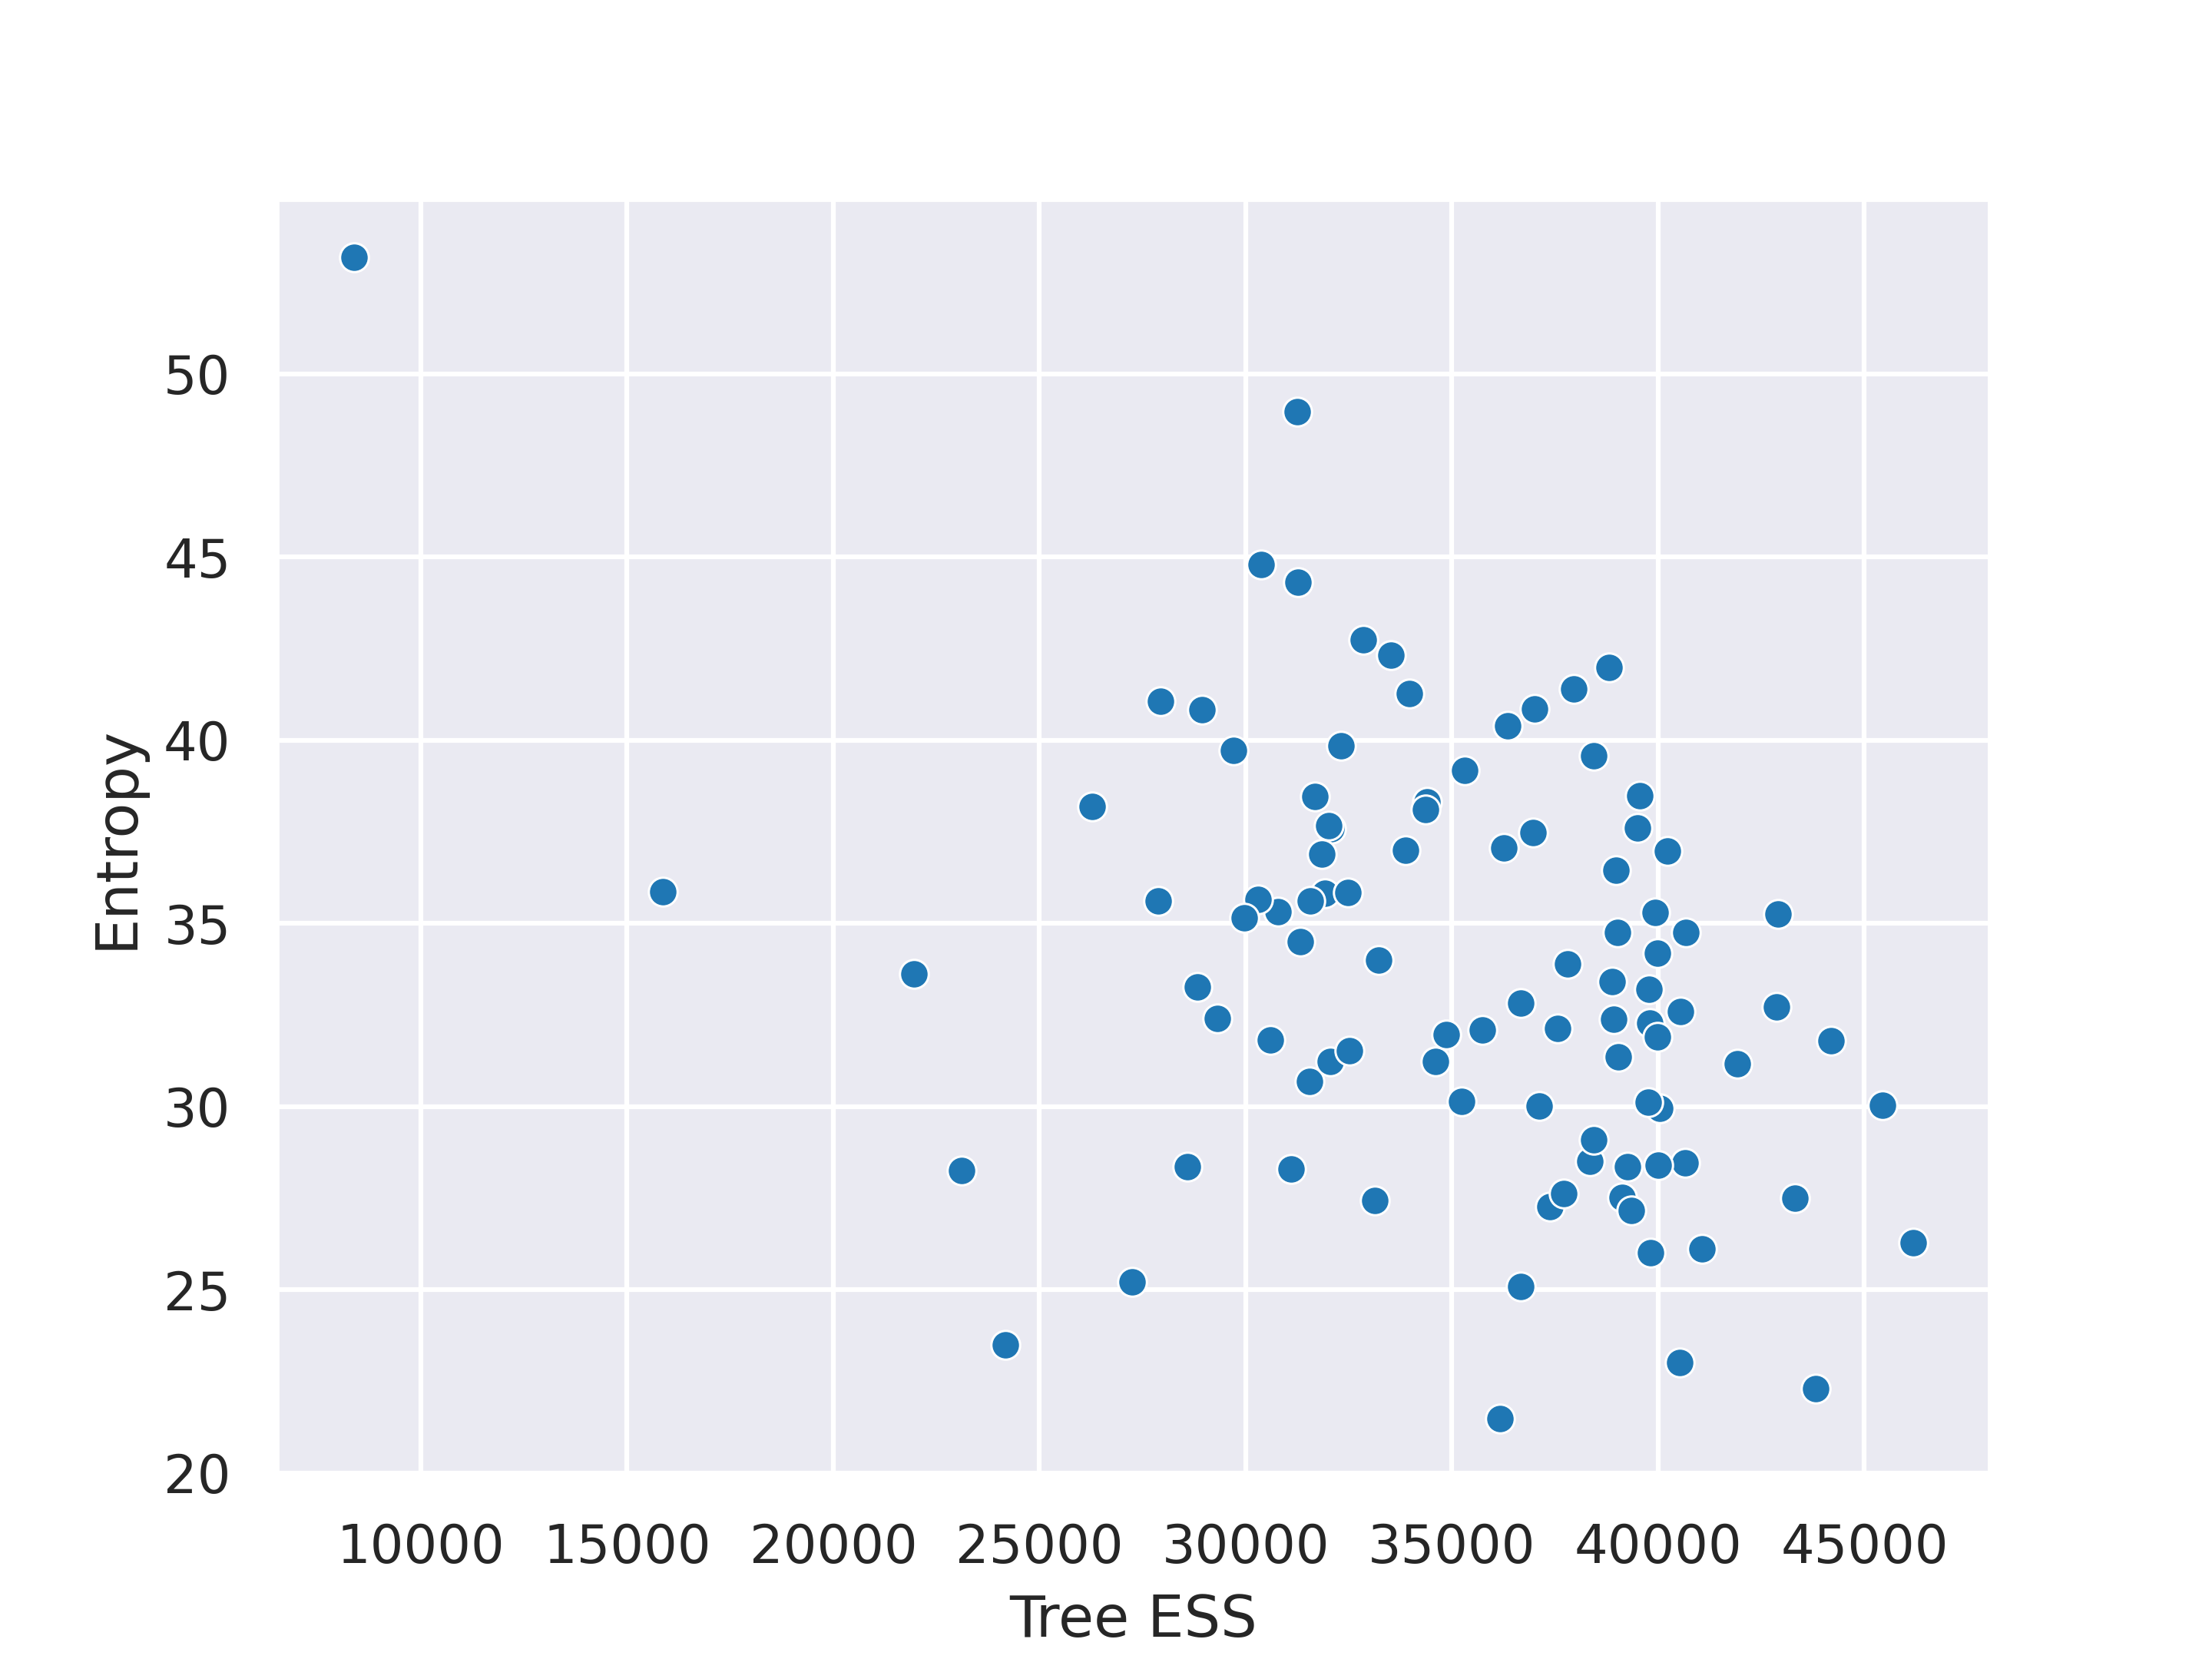
\includegraphics[width=\textwidth]{figures/yule-100-ccd1-entropy-ess.png}
		\subcaption{Yule-100}
	\end{subfigure}
	\begin{subfigure}[b]{0.4\textwidth}
		\centering
		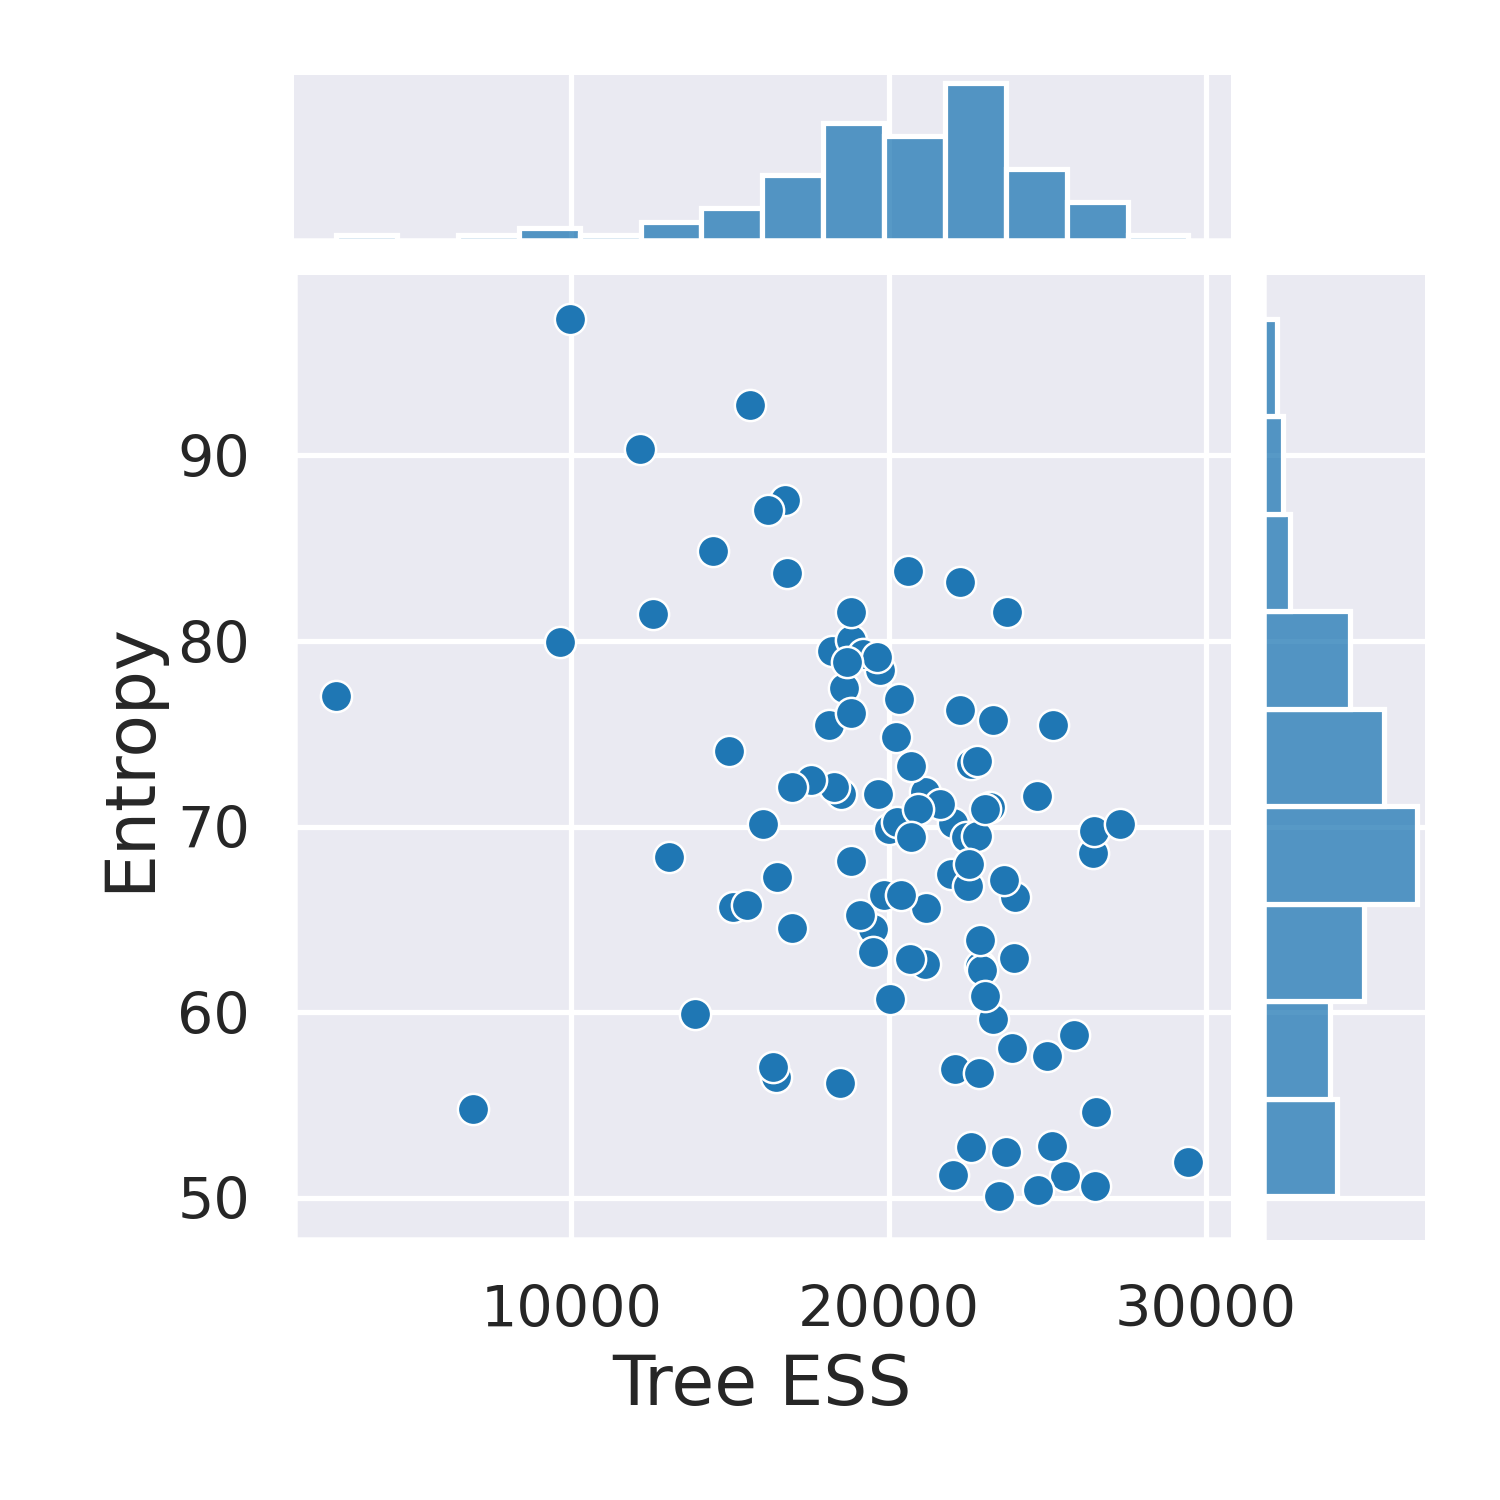
\includegraphics[width=\textwidth]{figures/yule-200-ccd1-entropy-ess.png}
		\subcaption{Yule-200}
	\end{subfigure}
	
	\begin{subfigure}[b]{0.4\textwidth}
		\centering
		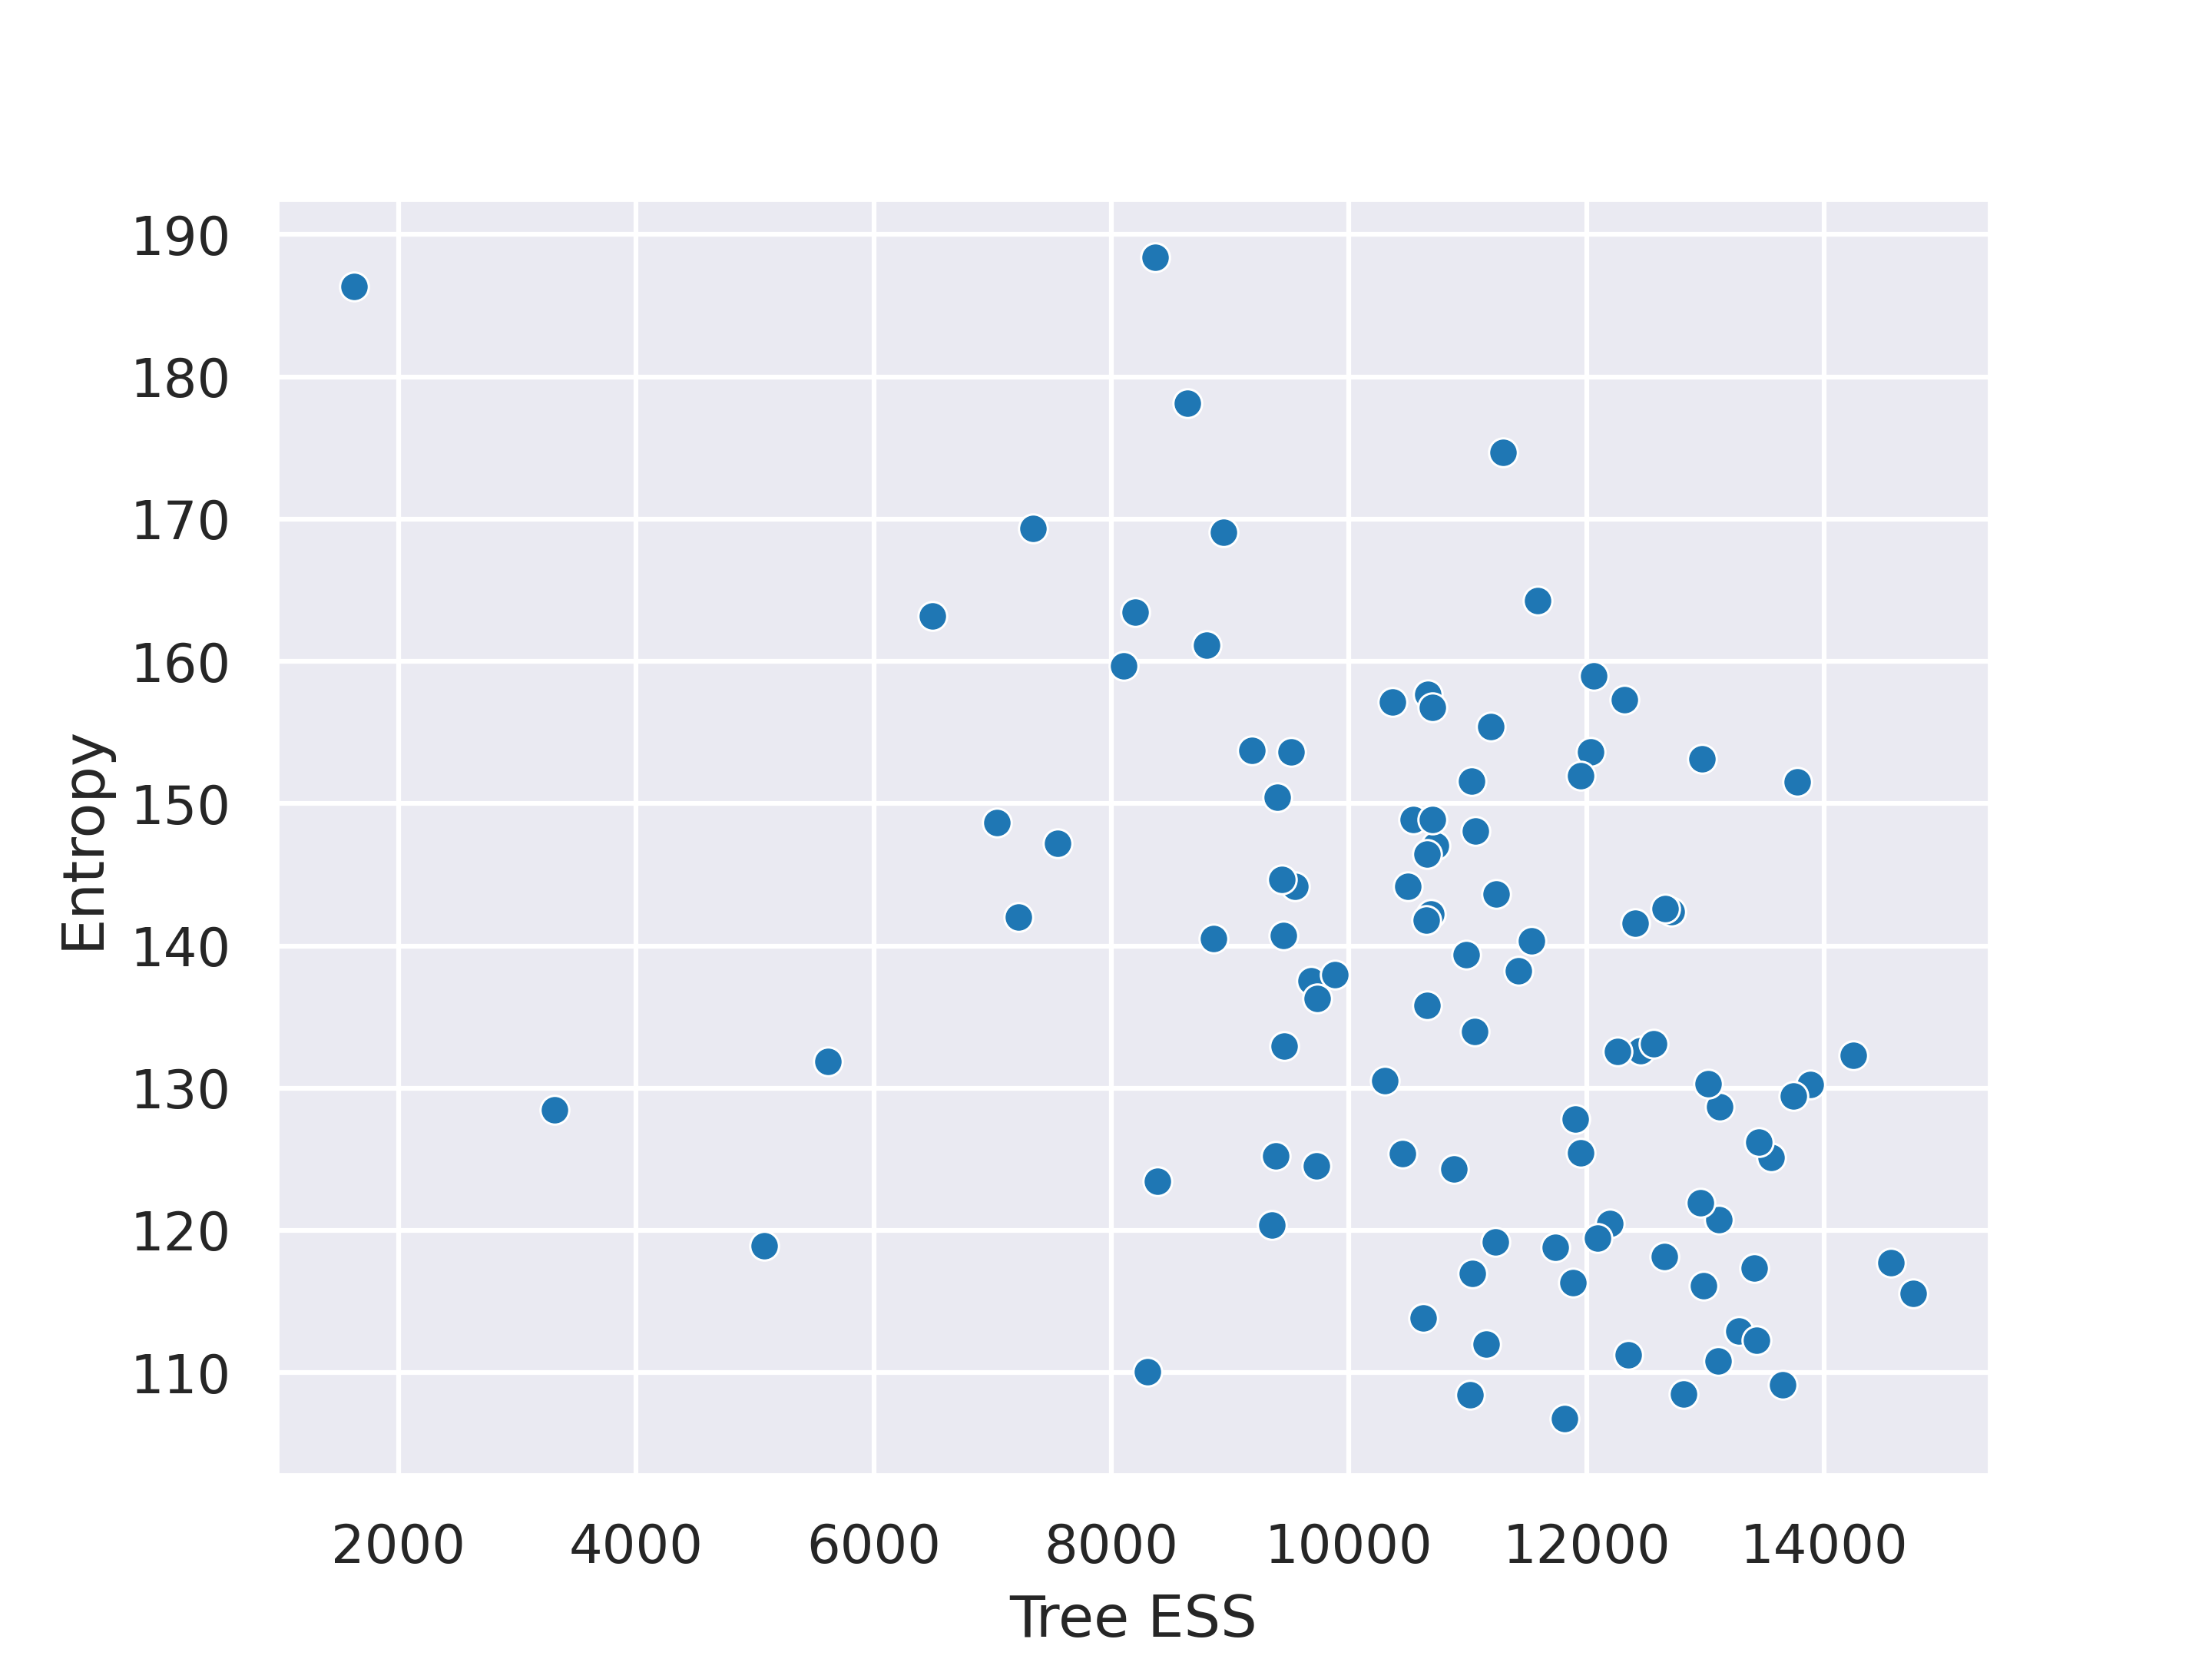
\includegraphics[width=\textwidth]{figures/yule-400-ccd1-entropy-ess.png}
		\subcaption{Yule-400}
	\end{subfigure}
	\begin{subfigure}[b]{0.4\textwidth}
		\centering
		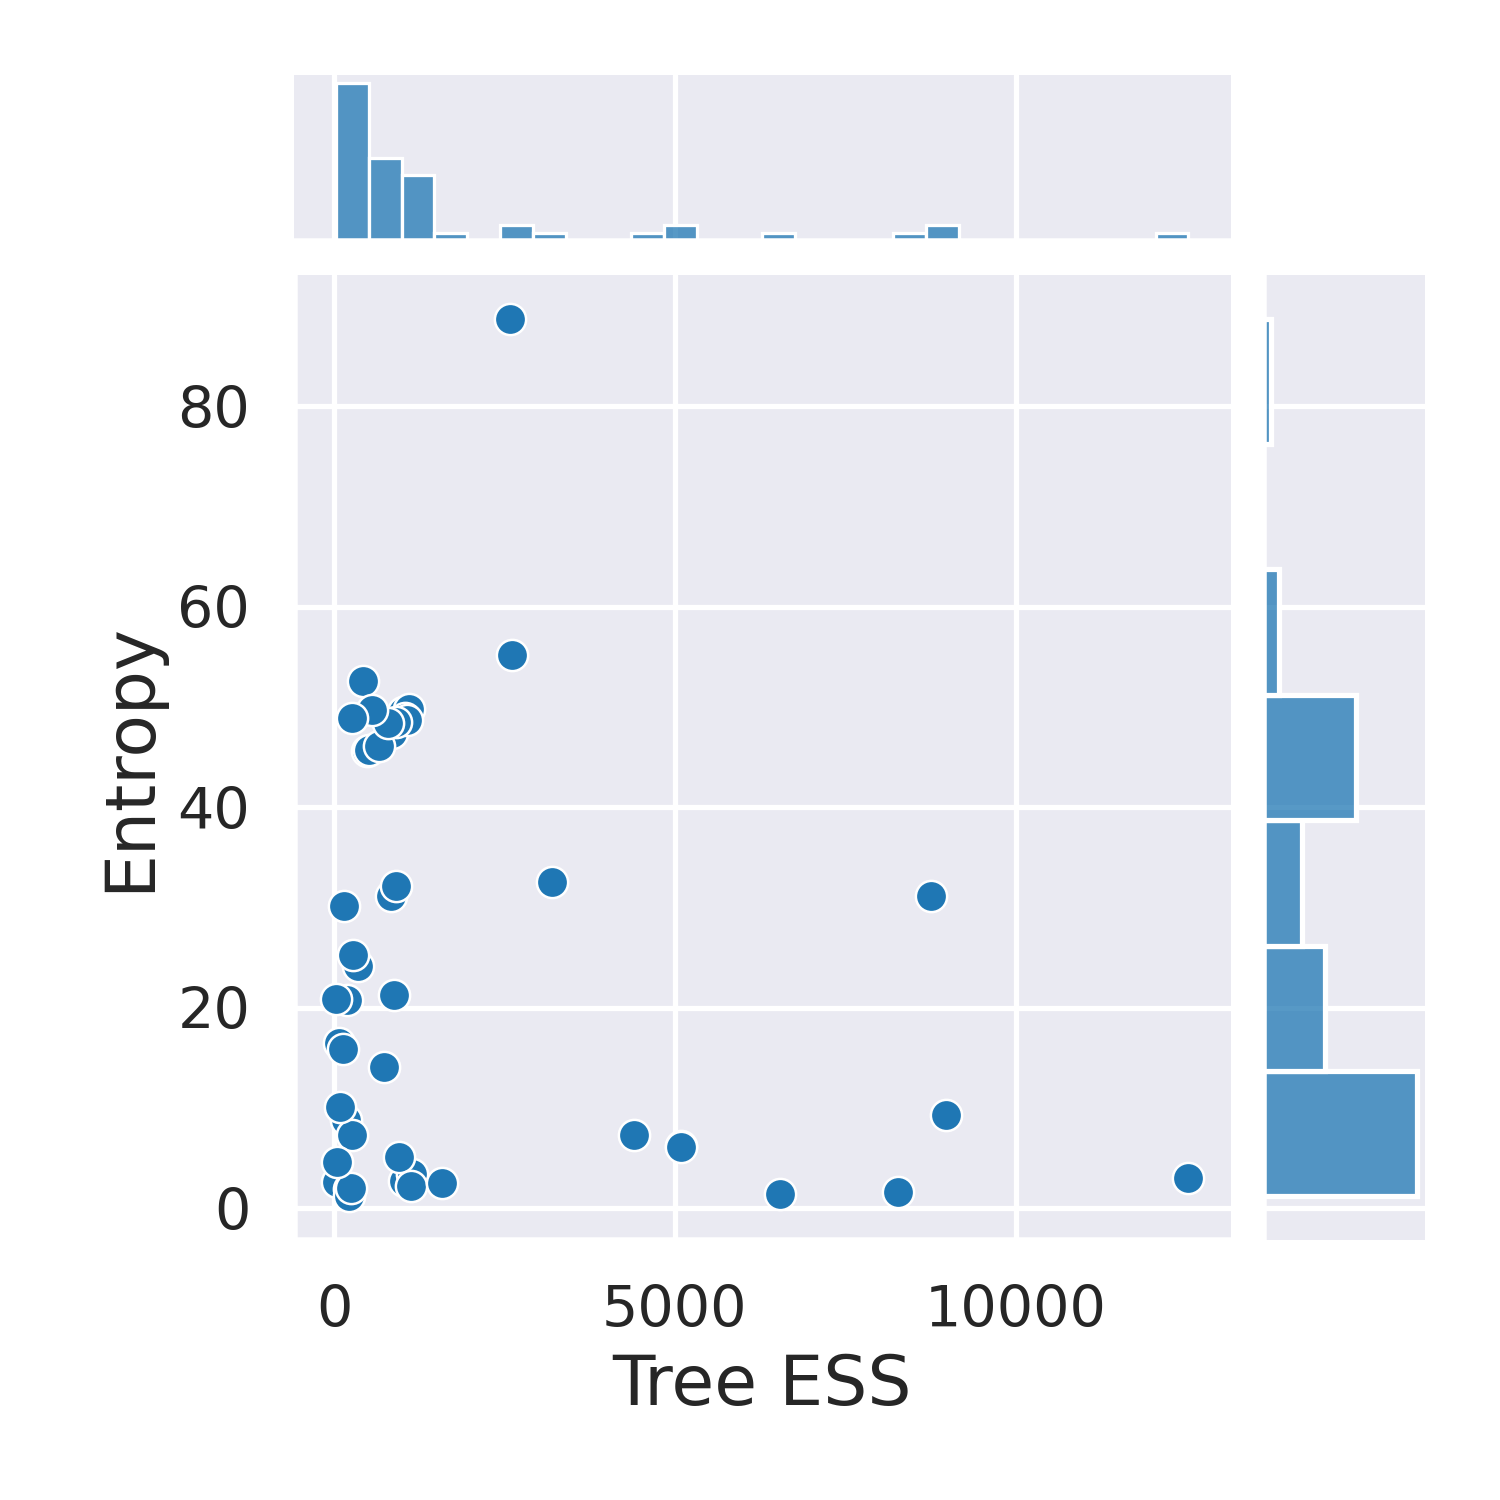
\includegraphics[width=\textwidth]{figures/bio-ccd1-entropy-ess.png}
		\subcaption{Real-world datasets}
	\end{subfigure}
	
	\label{fig:effective-sample-size-entropy}
\end{figure}

\subsection*{Data likelihood}

The first metric we consider to compare the different fitted distributions is the joint likelihood of the validation samples. Because we downsample the MCMC trees to their effective sample size, we can assume that the samples are independent. The joint data likelihood is thus given by the product of the probability for each tree in the validation set.

Figure \ref{fig:data-likelihood} shows the distribution of the log data likelihoods for the different distributions and datasets. There is a clear pattern where the height ratio distributions have the highest likelihood, followed by the shortest branch and last divergence embeddings. This pattern is also visible when looking at the ranking of each method for every single MCMC sample in figure \ref{fig:data-likelihood-ranking}: these plots show for many datasets each distribution is at a specific rank when sorting the distributions by their log data likelihood.

\begin{figure}
	\caption{The log data likelihoods for the different distributions and datasets. (The higher the better.)}
	
	\centering
	\begin{subfigure}[b]{0.45\textwidth}
		\centering
		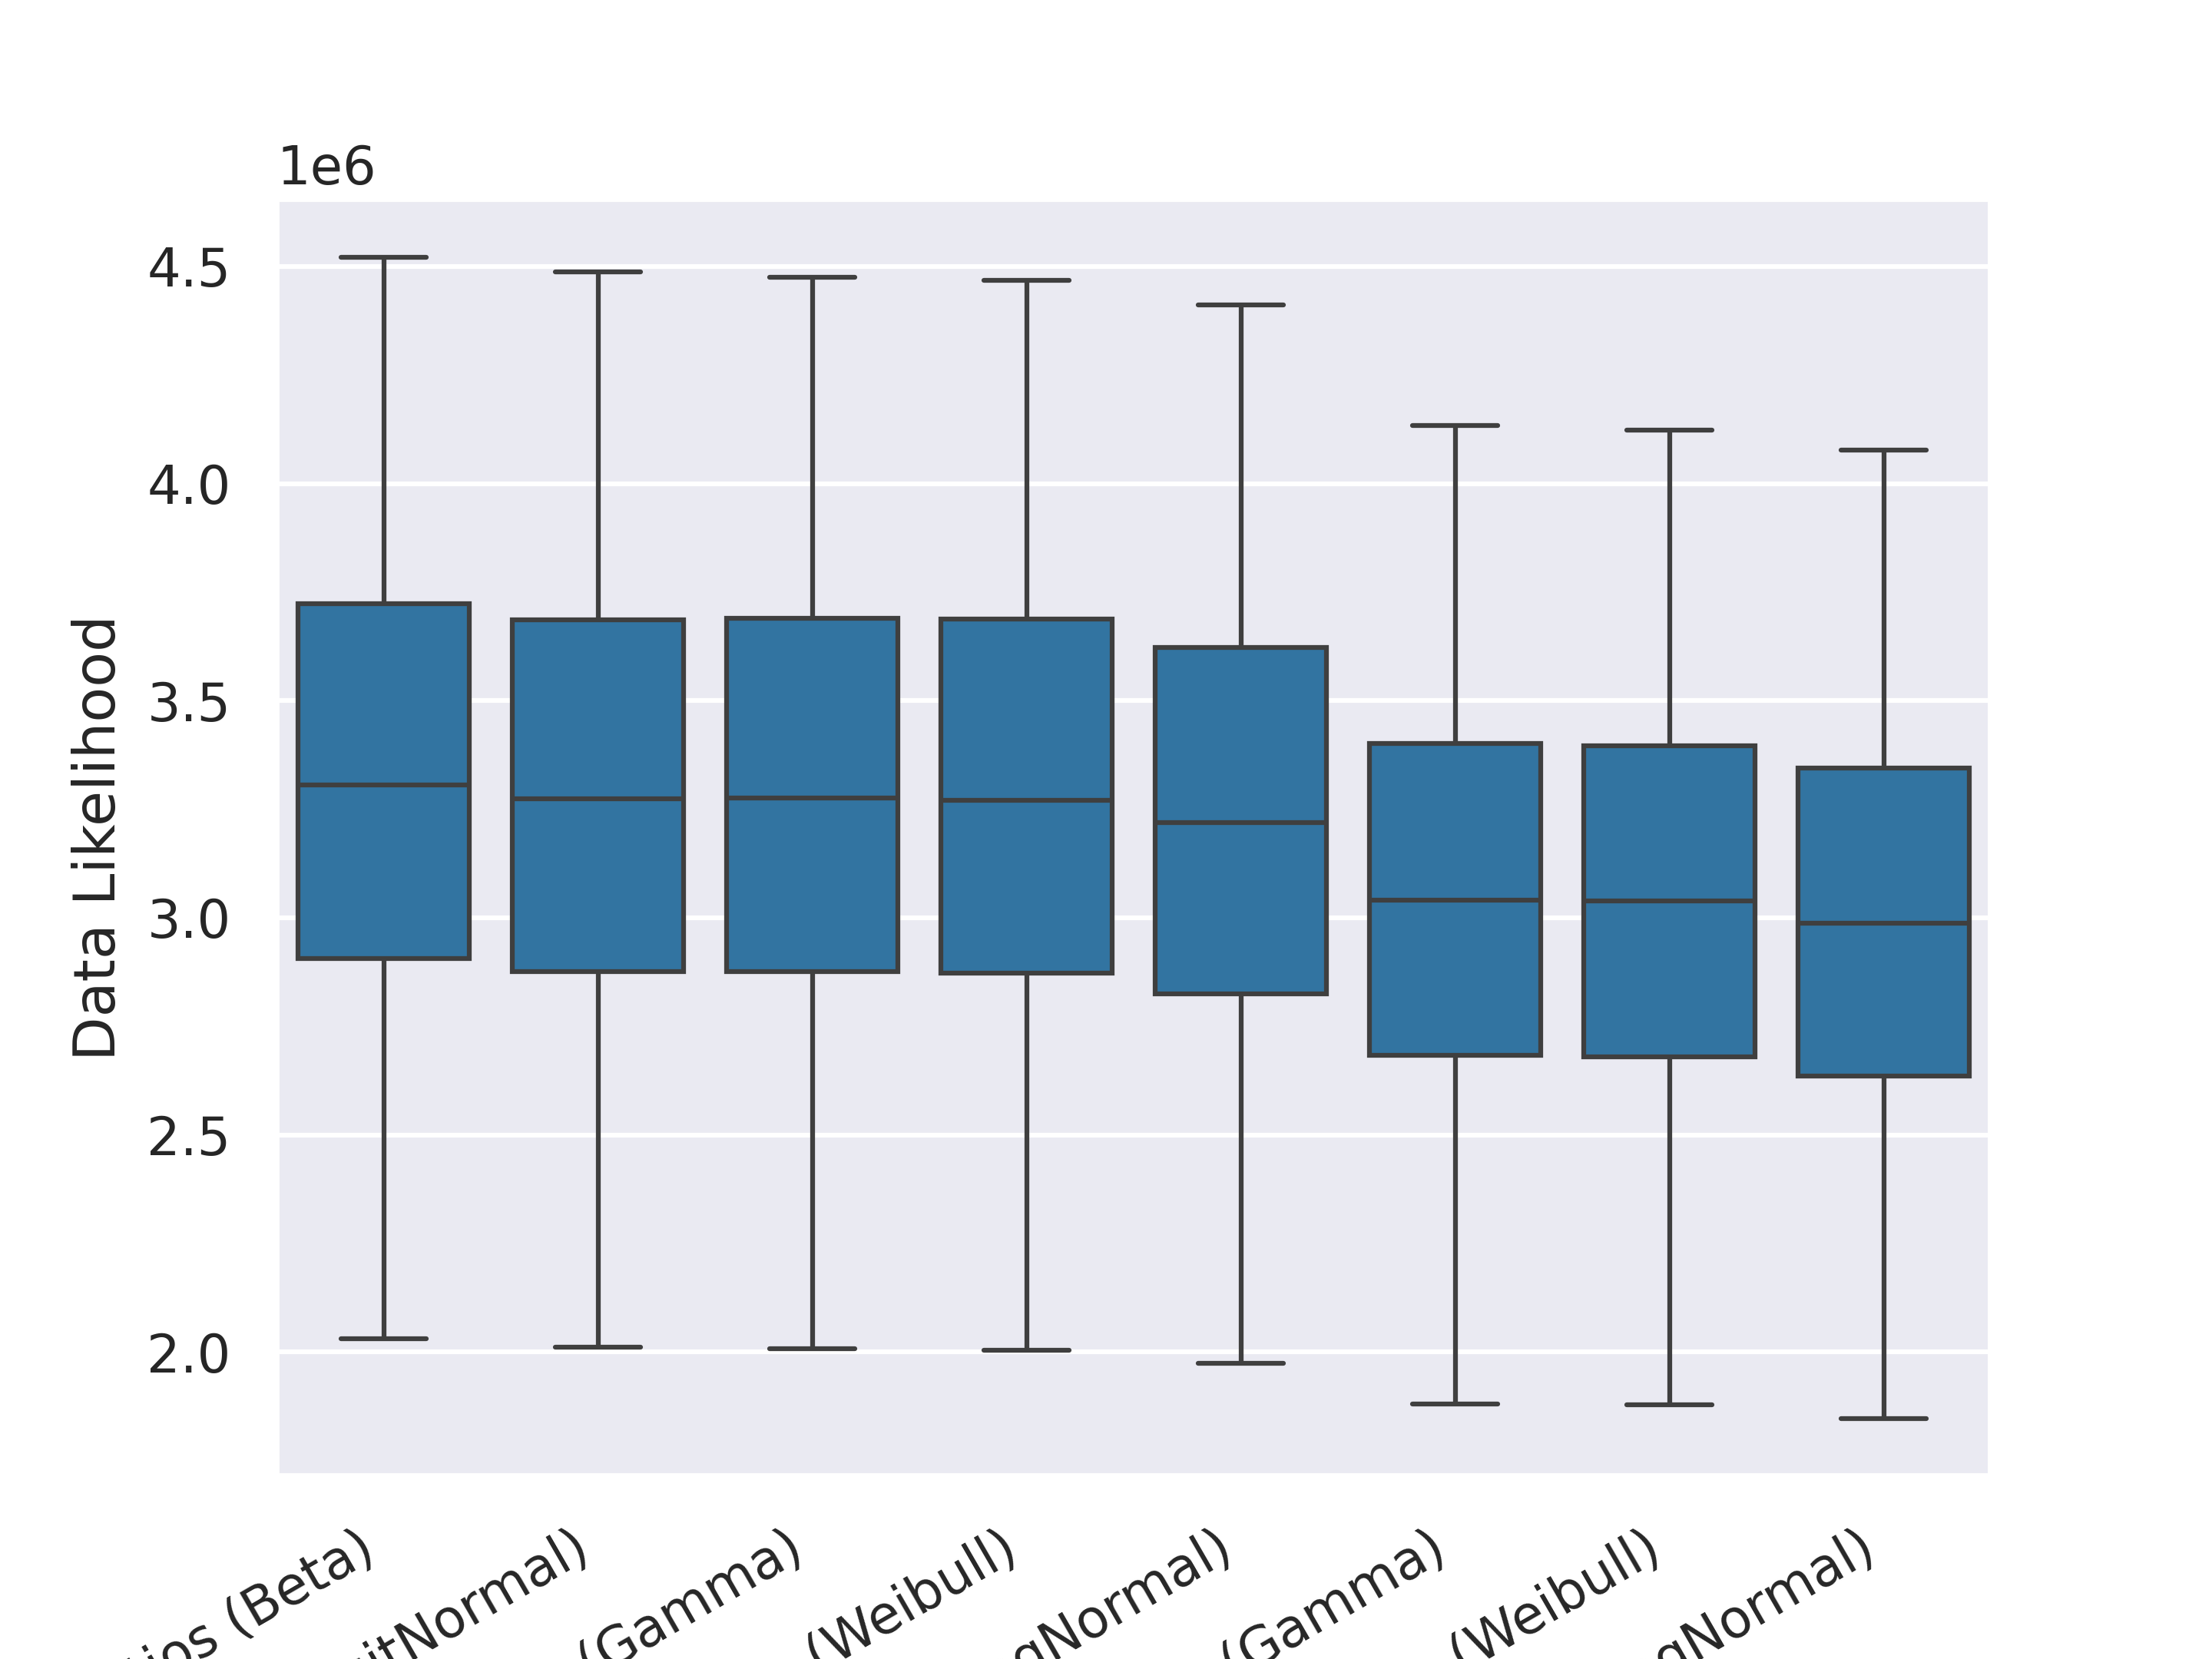
\includegraphics[width=\textwidth]{figures/yule-100-ccd1-likelihood.png}
		\subcaption{Yule-100}
	\end{subfigure}
	\begin{subfigure}[b]{0.45\textwidth}
		\centering
		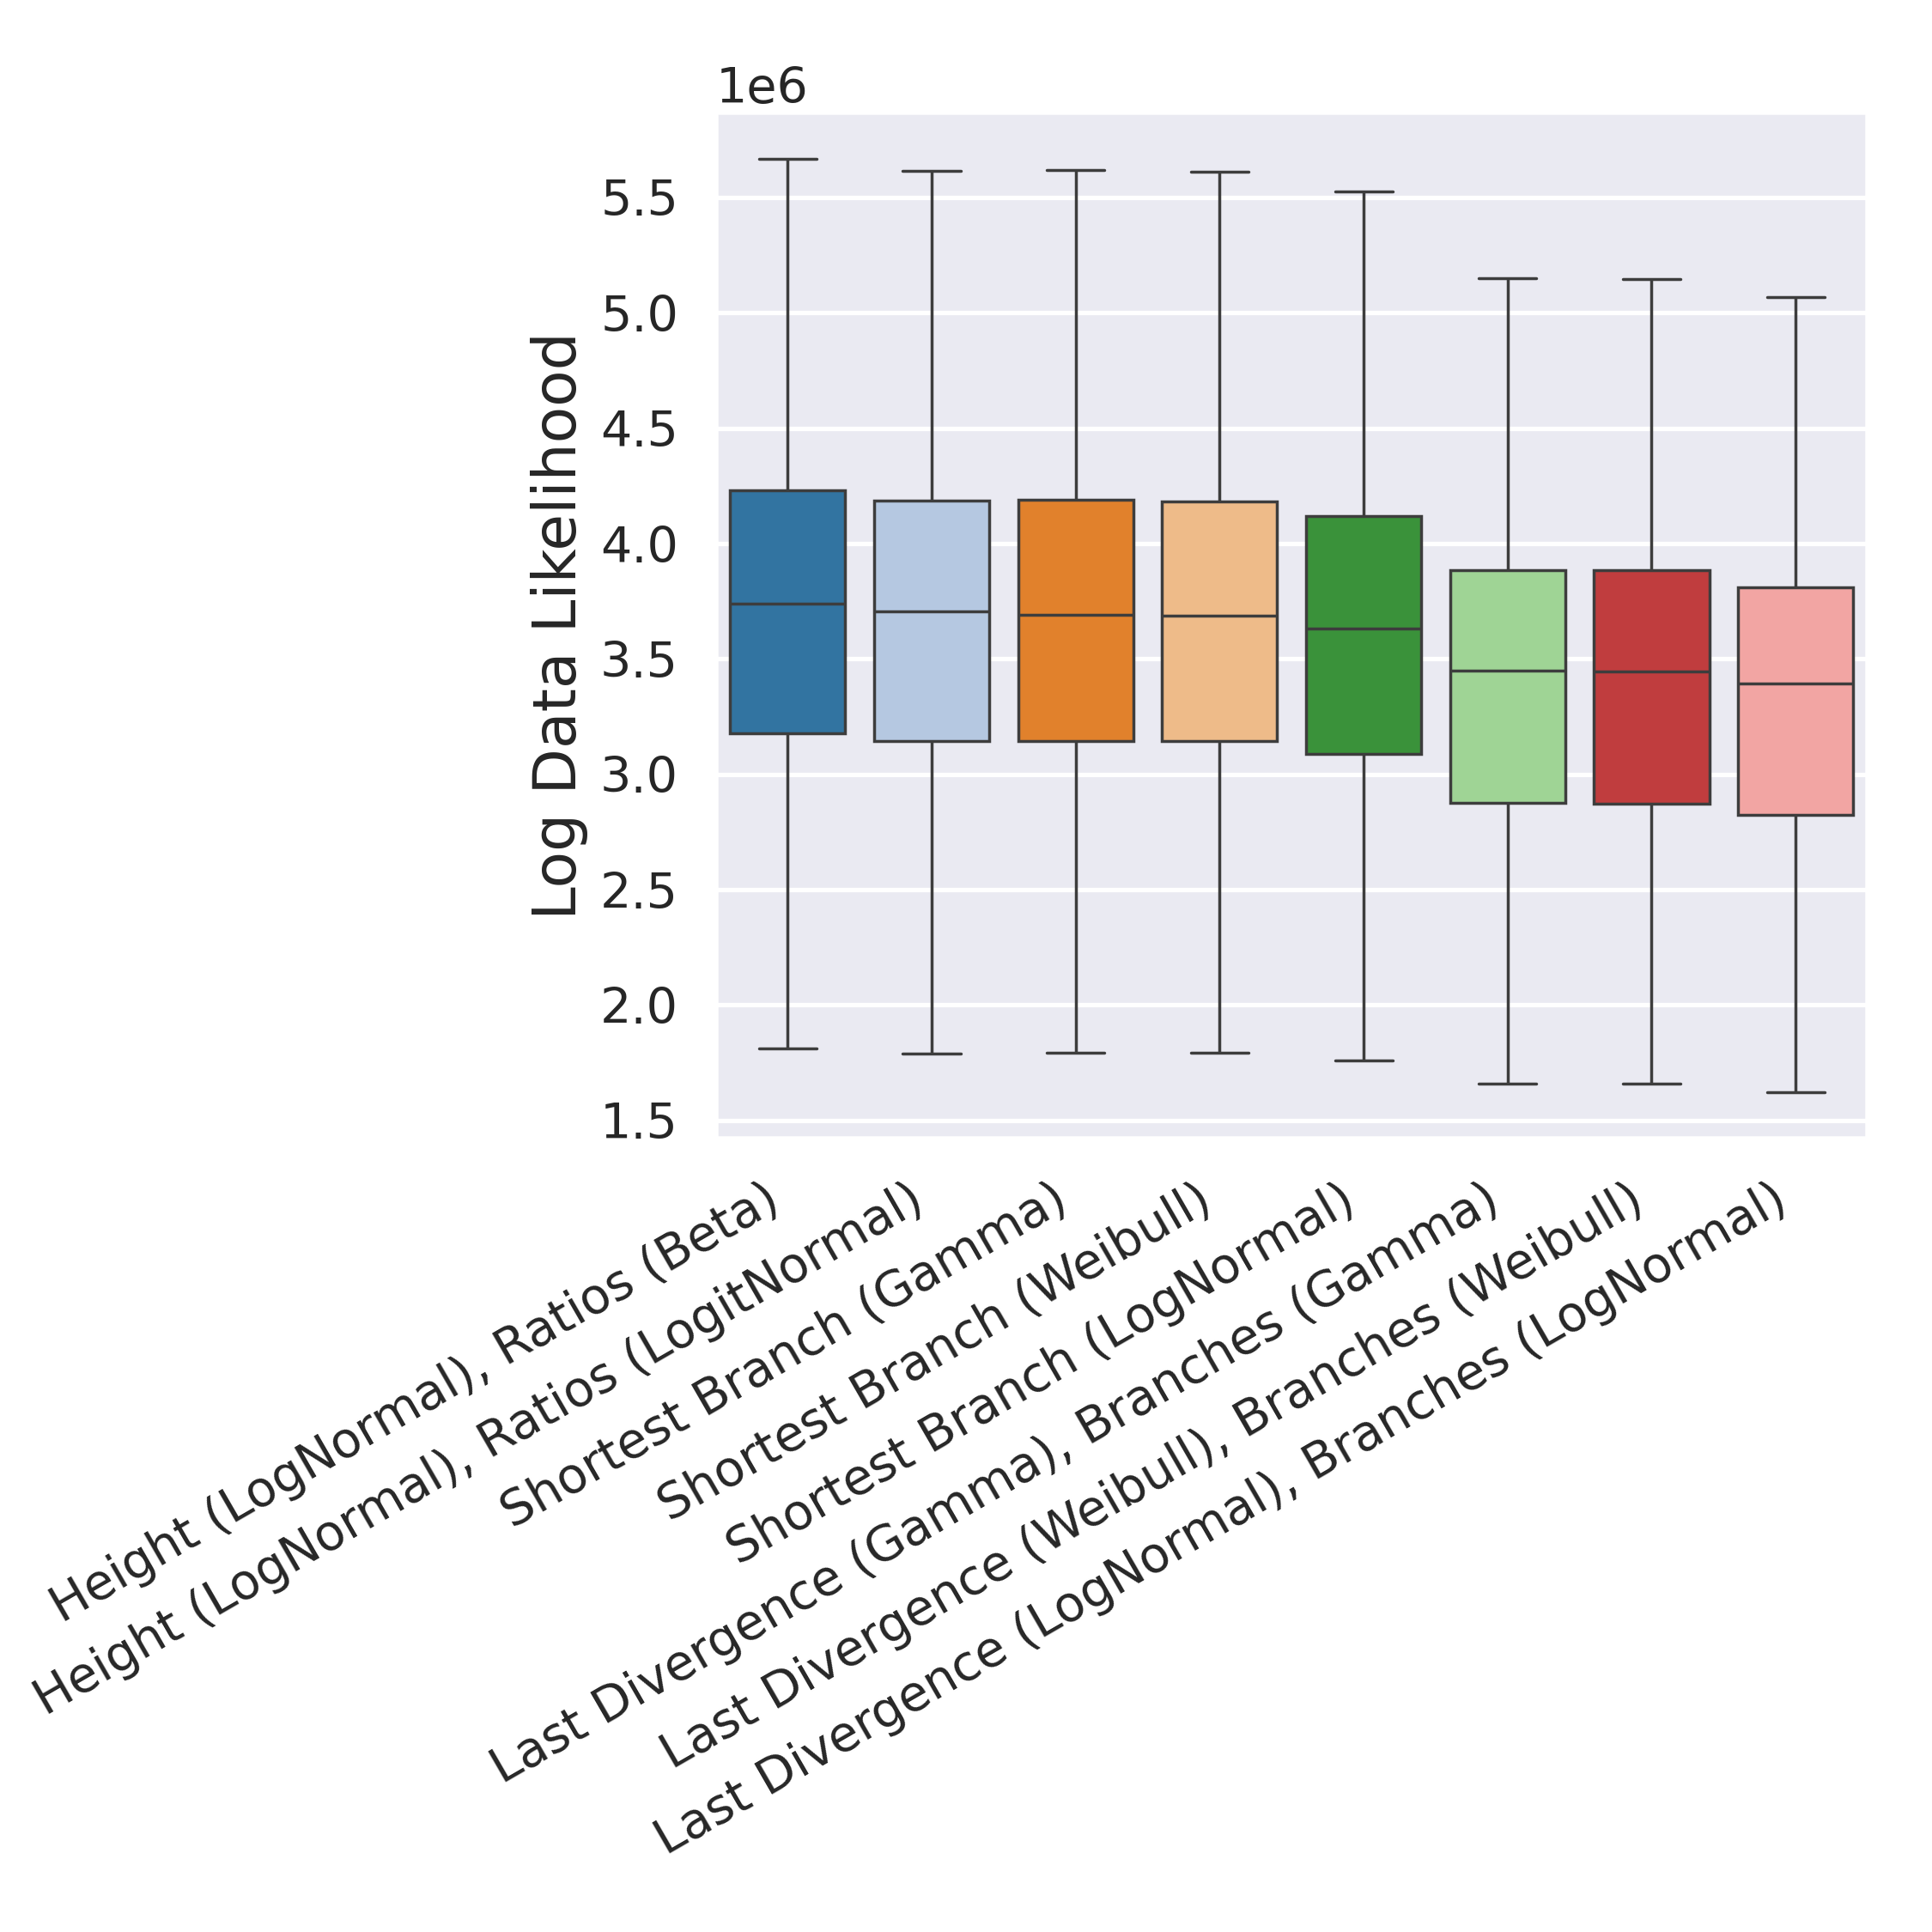
\includegraphics[width=\textwidth]{figures/yule-200-ccd1-likelihood.png}
		\subcaption{Yule-200}
	\end{subfigure}
	
	\begin{subfigure}[b]{0.45\textwidth}
		\centering
		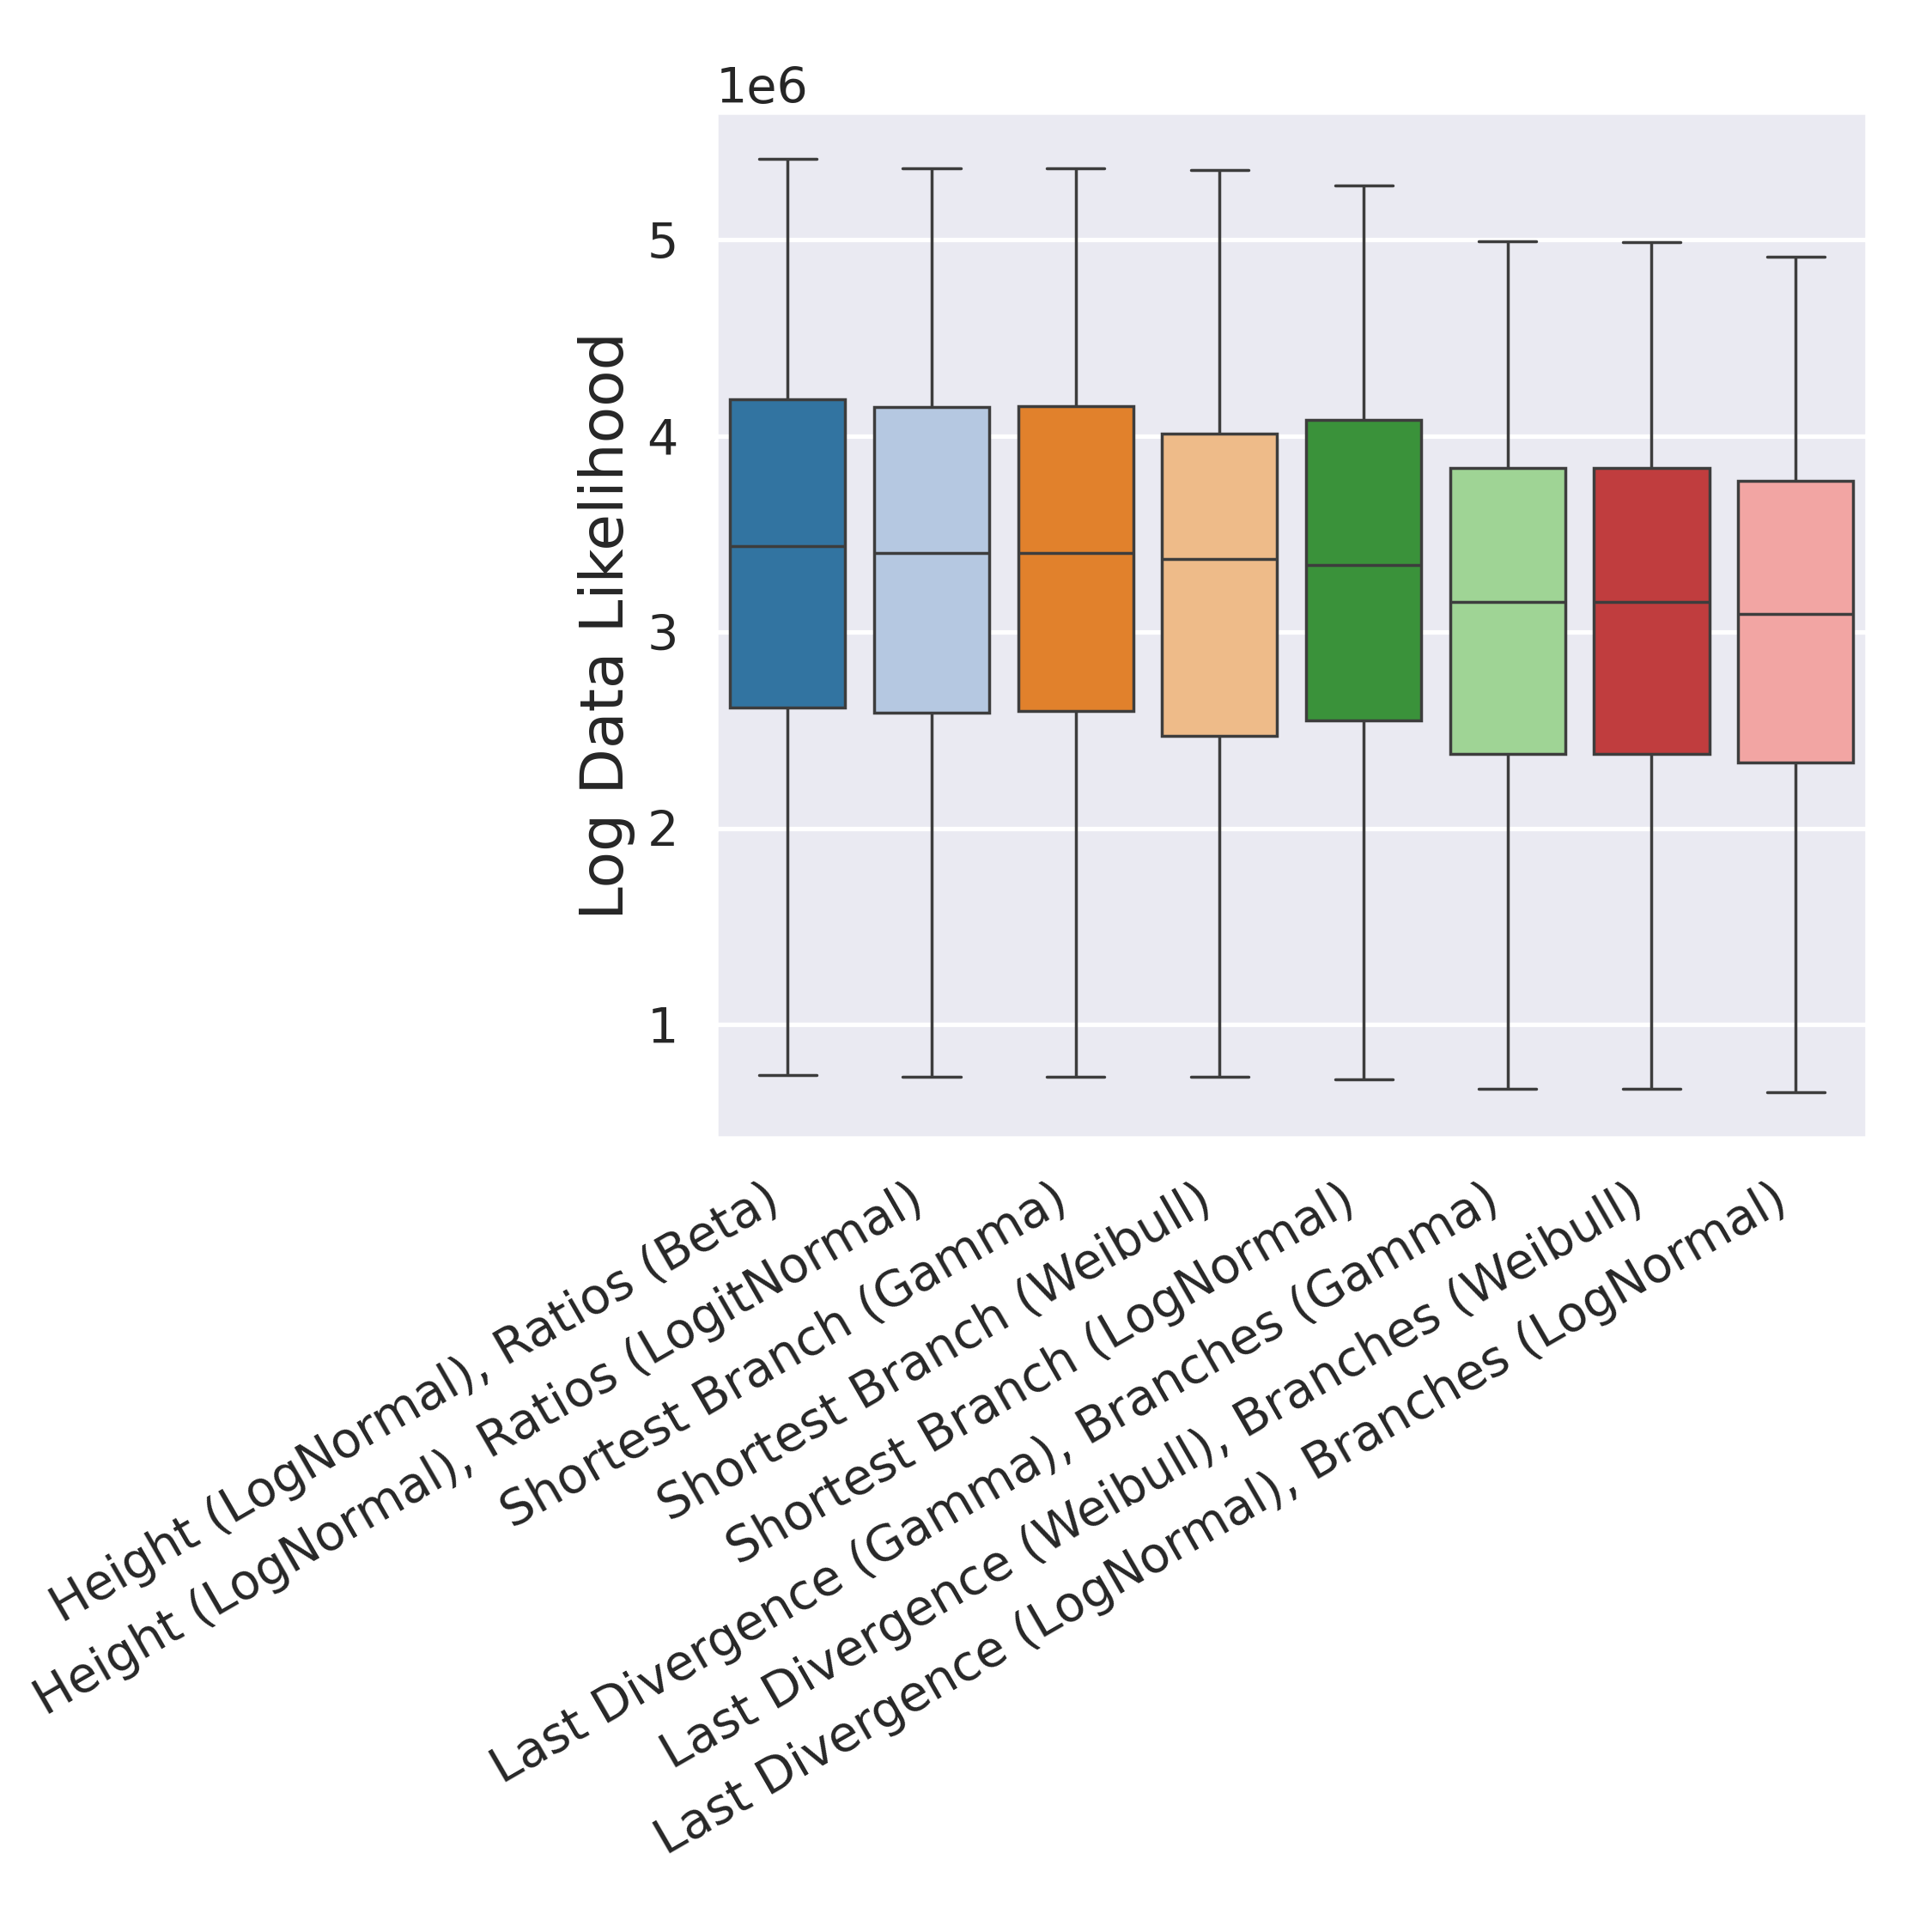
\includegraphics[width=\textwidth]{figures/yule-400-ccd1-likelihood.png}
		\subcaption{Yule-400}
	\end{subfigure}
	\begin{subfigure}[b]{0.45\textwidth}
		\centering
		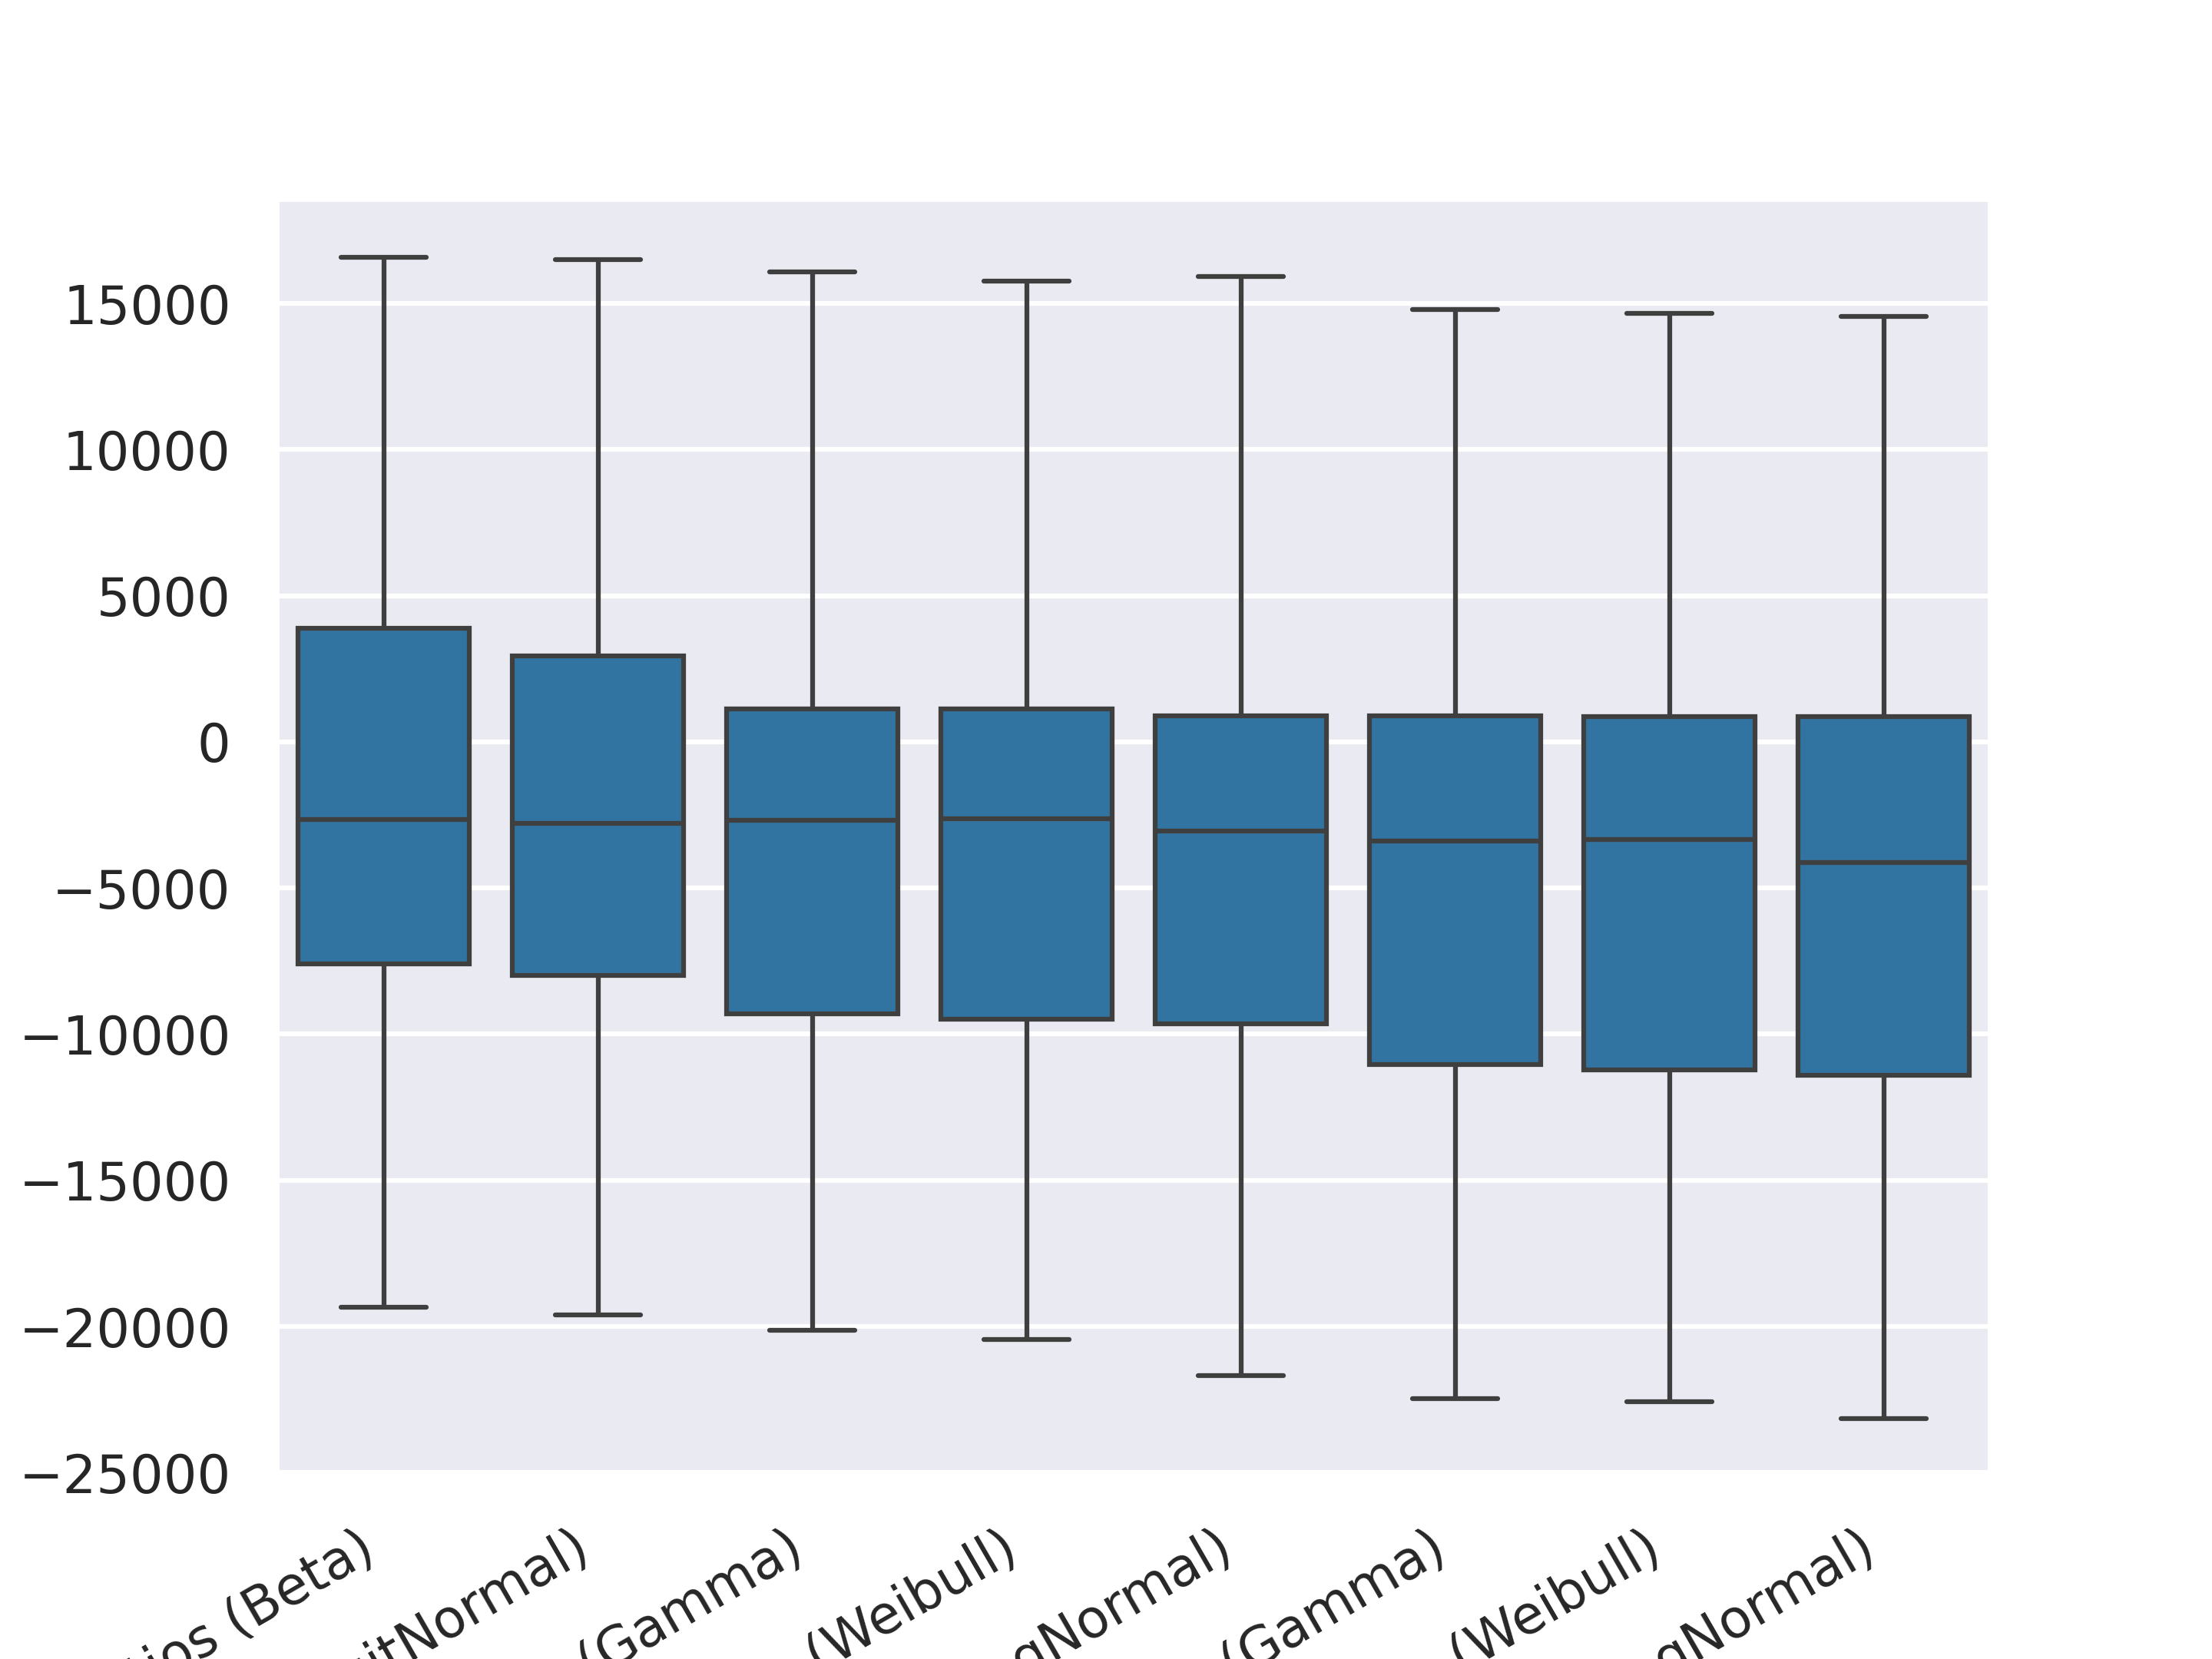
\includegraphics[width=\textwidth]{figures/bio-ccd1-likelihood.png}
		\subcaption{Real-world datasets}
	\end{subfigure}
	
	\label{fig:data-likelihood}
\end{figure}

\begin{figure}
	\caption{How often a specific method likelihood ranks at a certain position when compared to the other methods. For example, the height ratio embedding with the beta distribution ranks first for almost all datasets. (The lower the rank the better.)}
	
	\centering
	\begin{subfigure}[b]{0.45\textwidth}
		\centering
		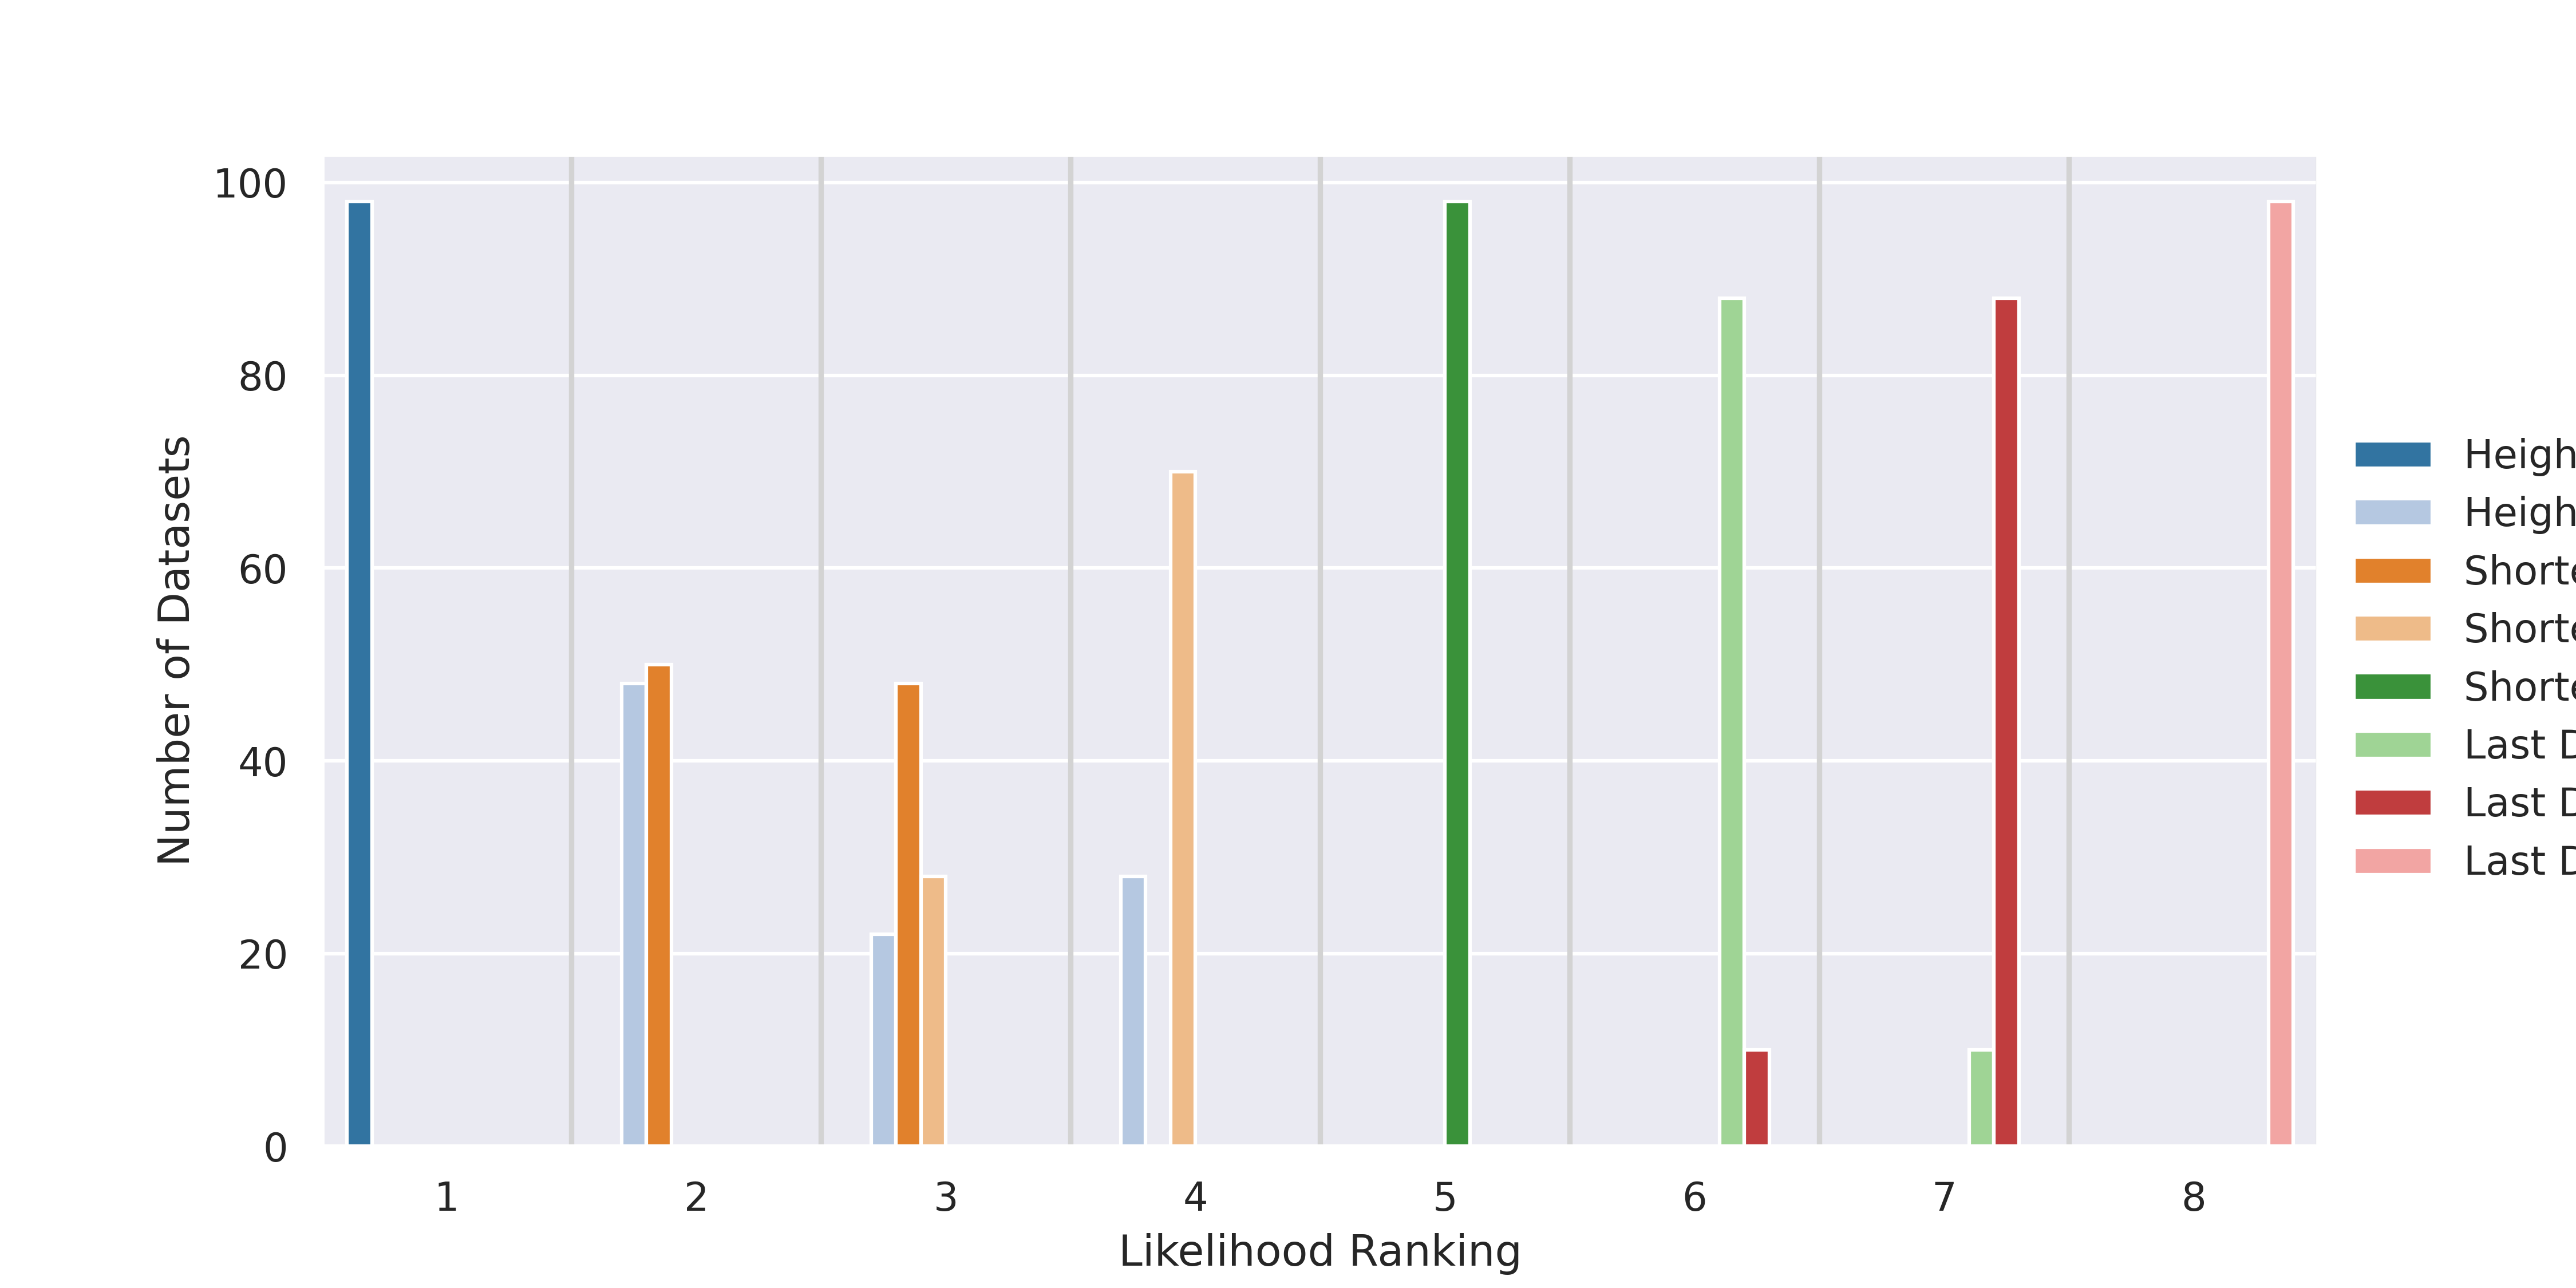
\includegraphics[width=\textwidth]{figures/yule-100-ccd1-likelihood-ranking.png}
		\subcaption{Yule-100}
	\end{subfigure}
	\begin{subfigure}[b]{0.45\textwidth}
		\centering
		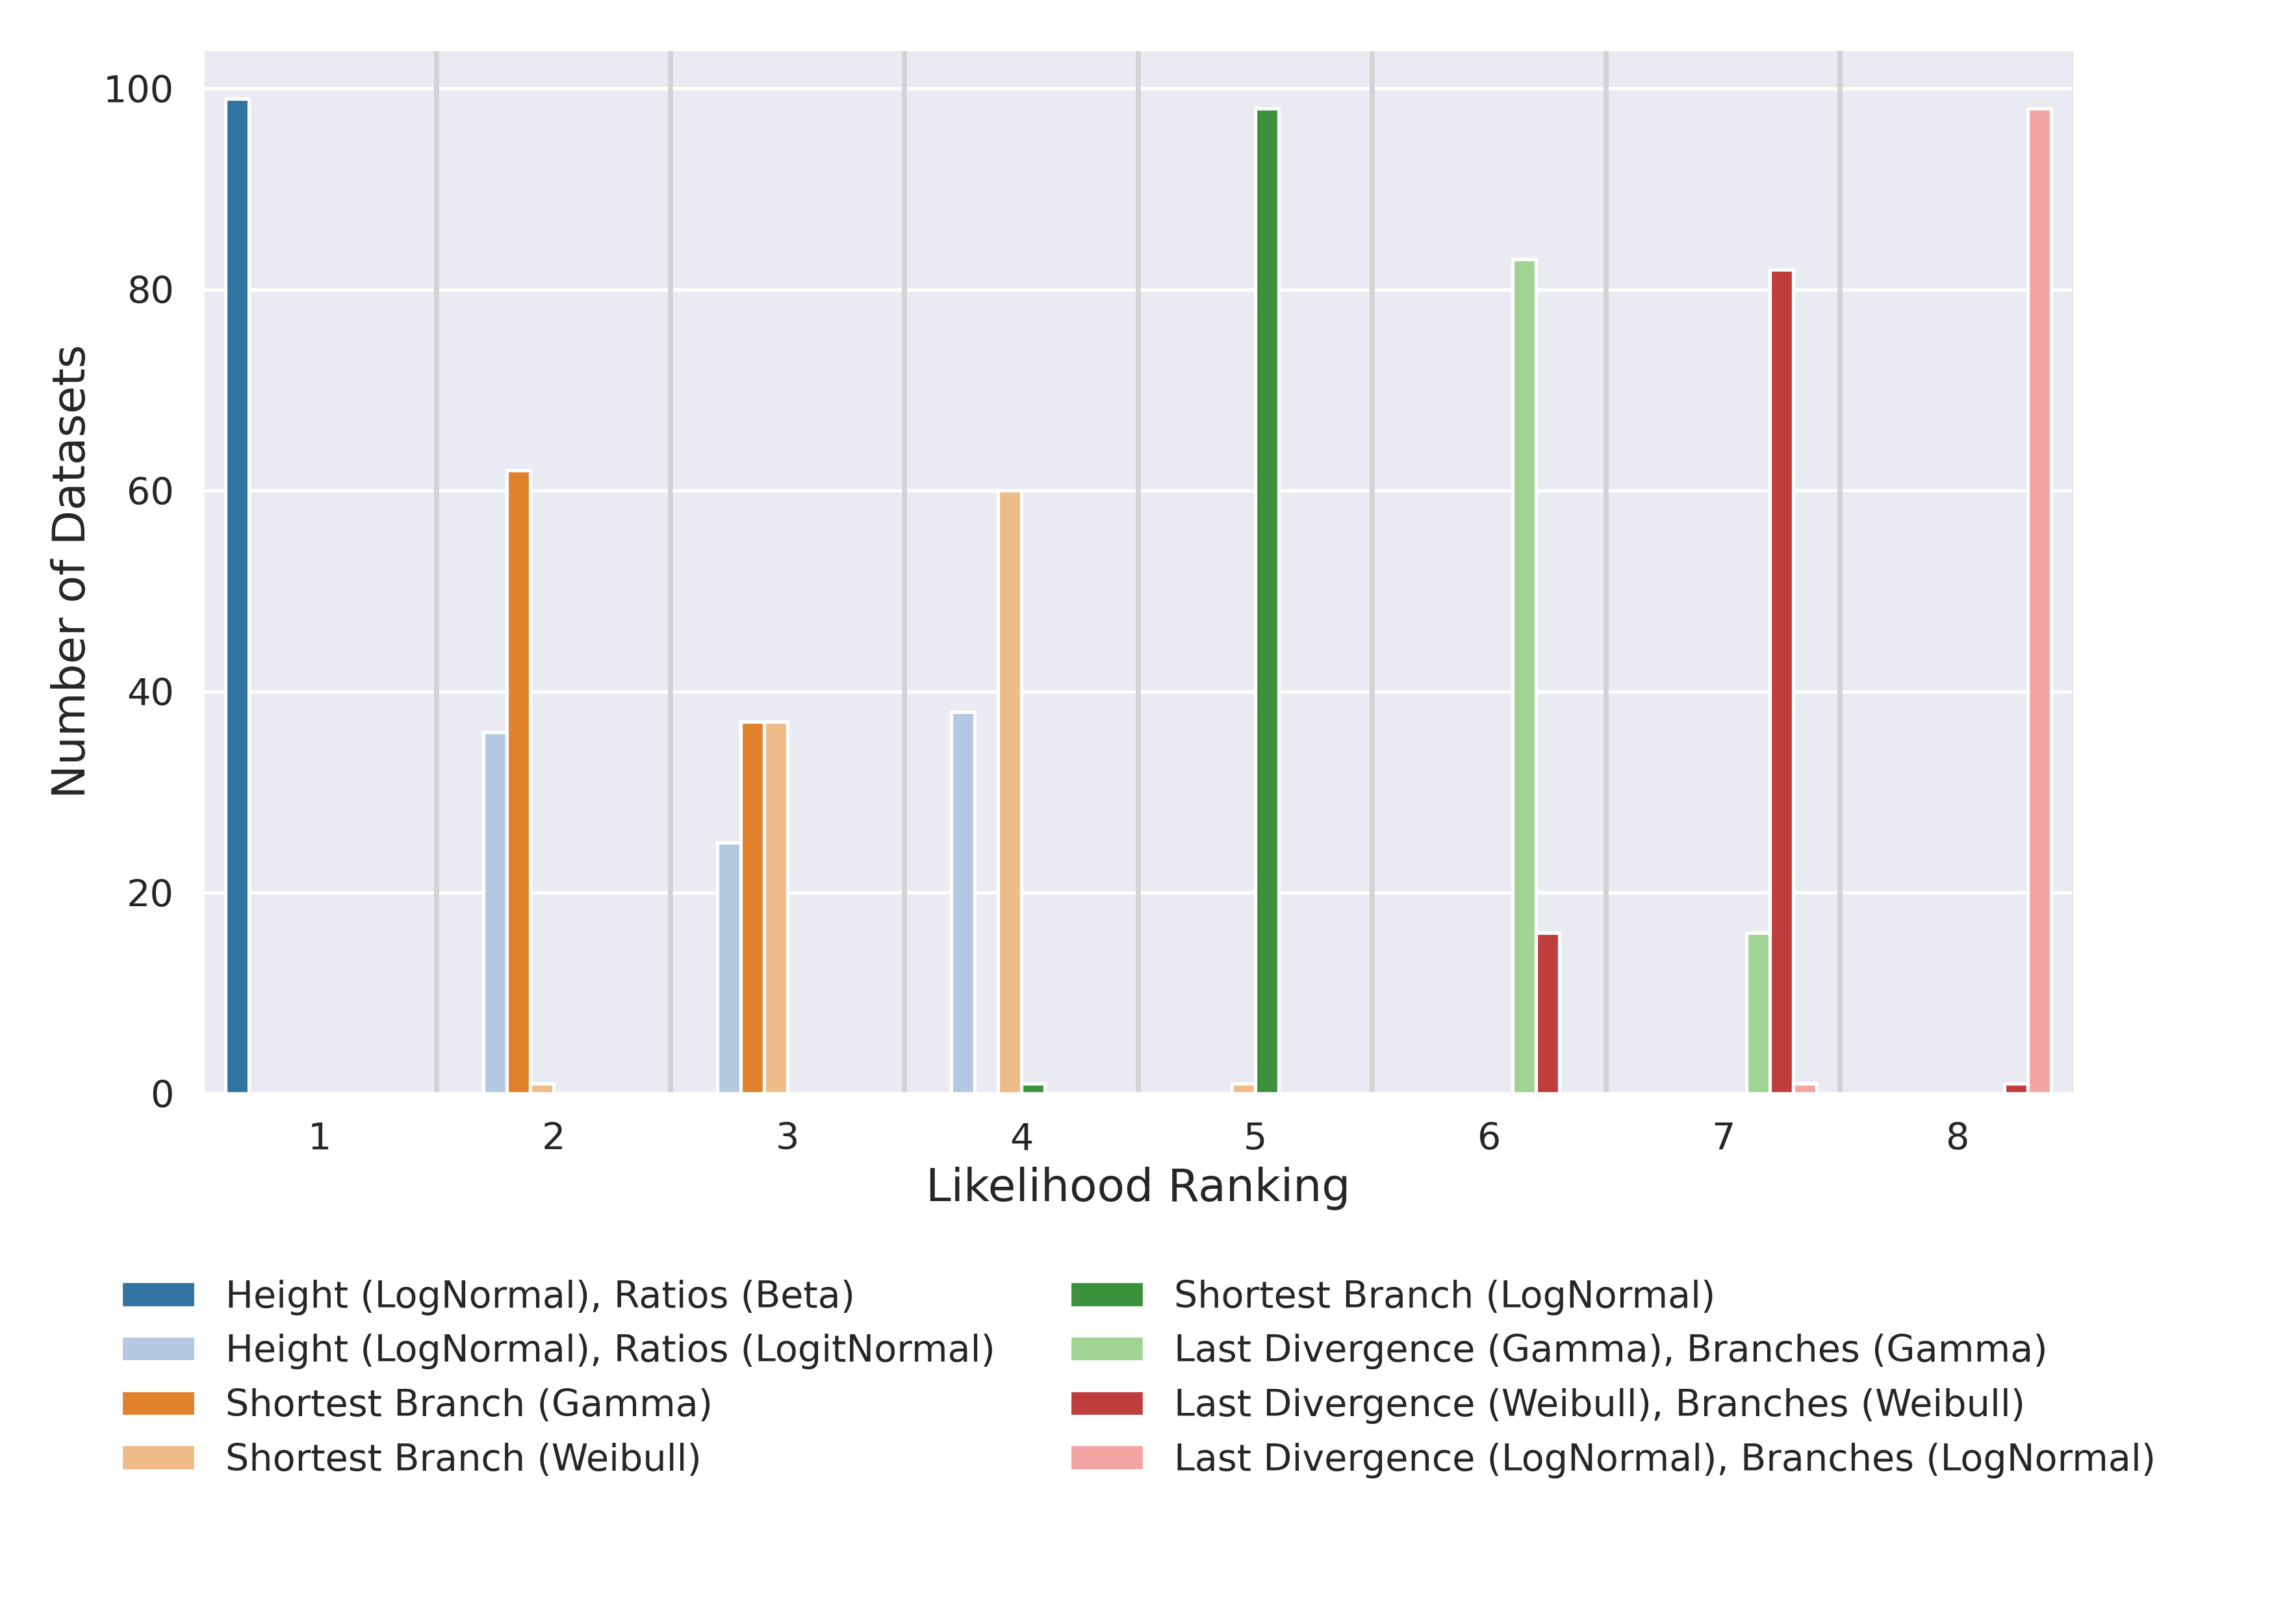
\includegraphics[width=\textwidth]{figures/yule-200-ccd1-likelihood-ranking.png}
		\subcaption{Yule-200}
	\end{subfigure}
	
	\begin{subfigure}[b]{0.45\textwidth}
		\centering
		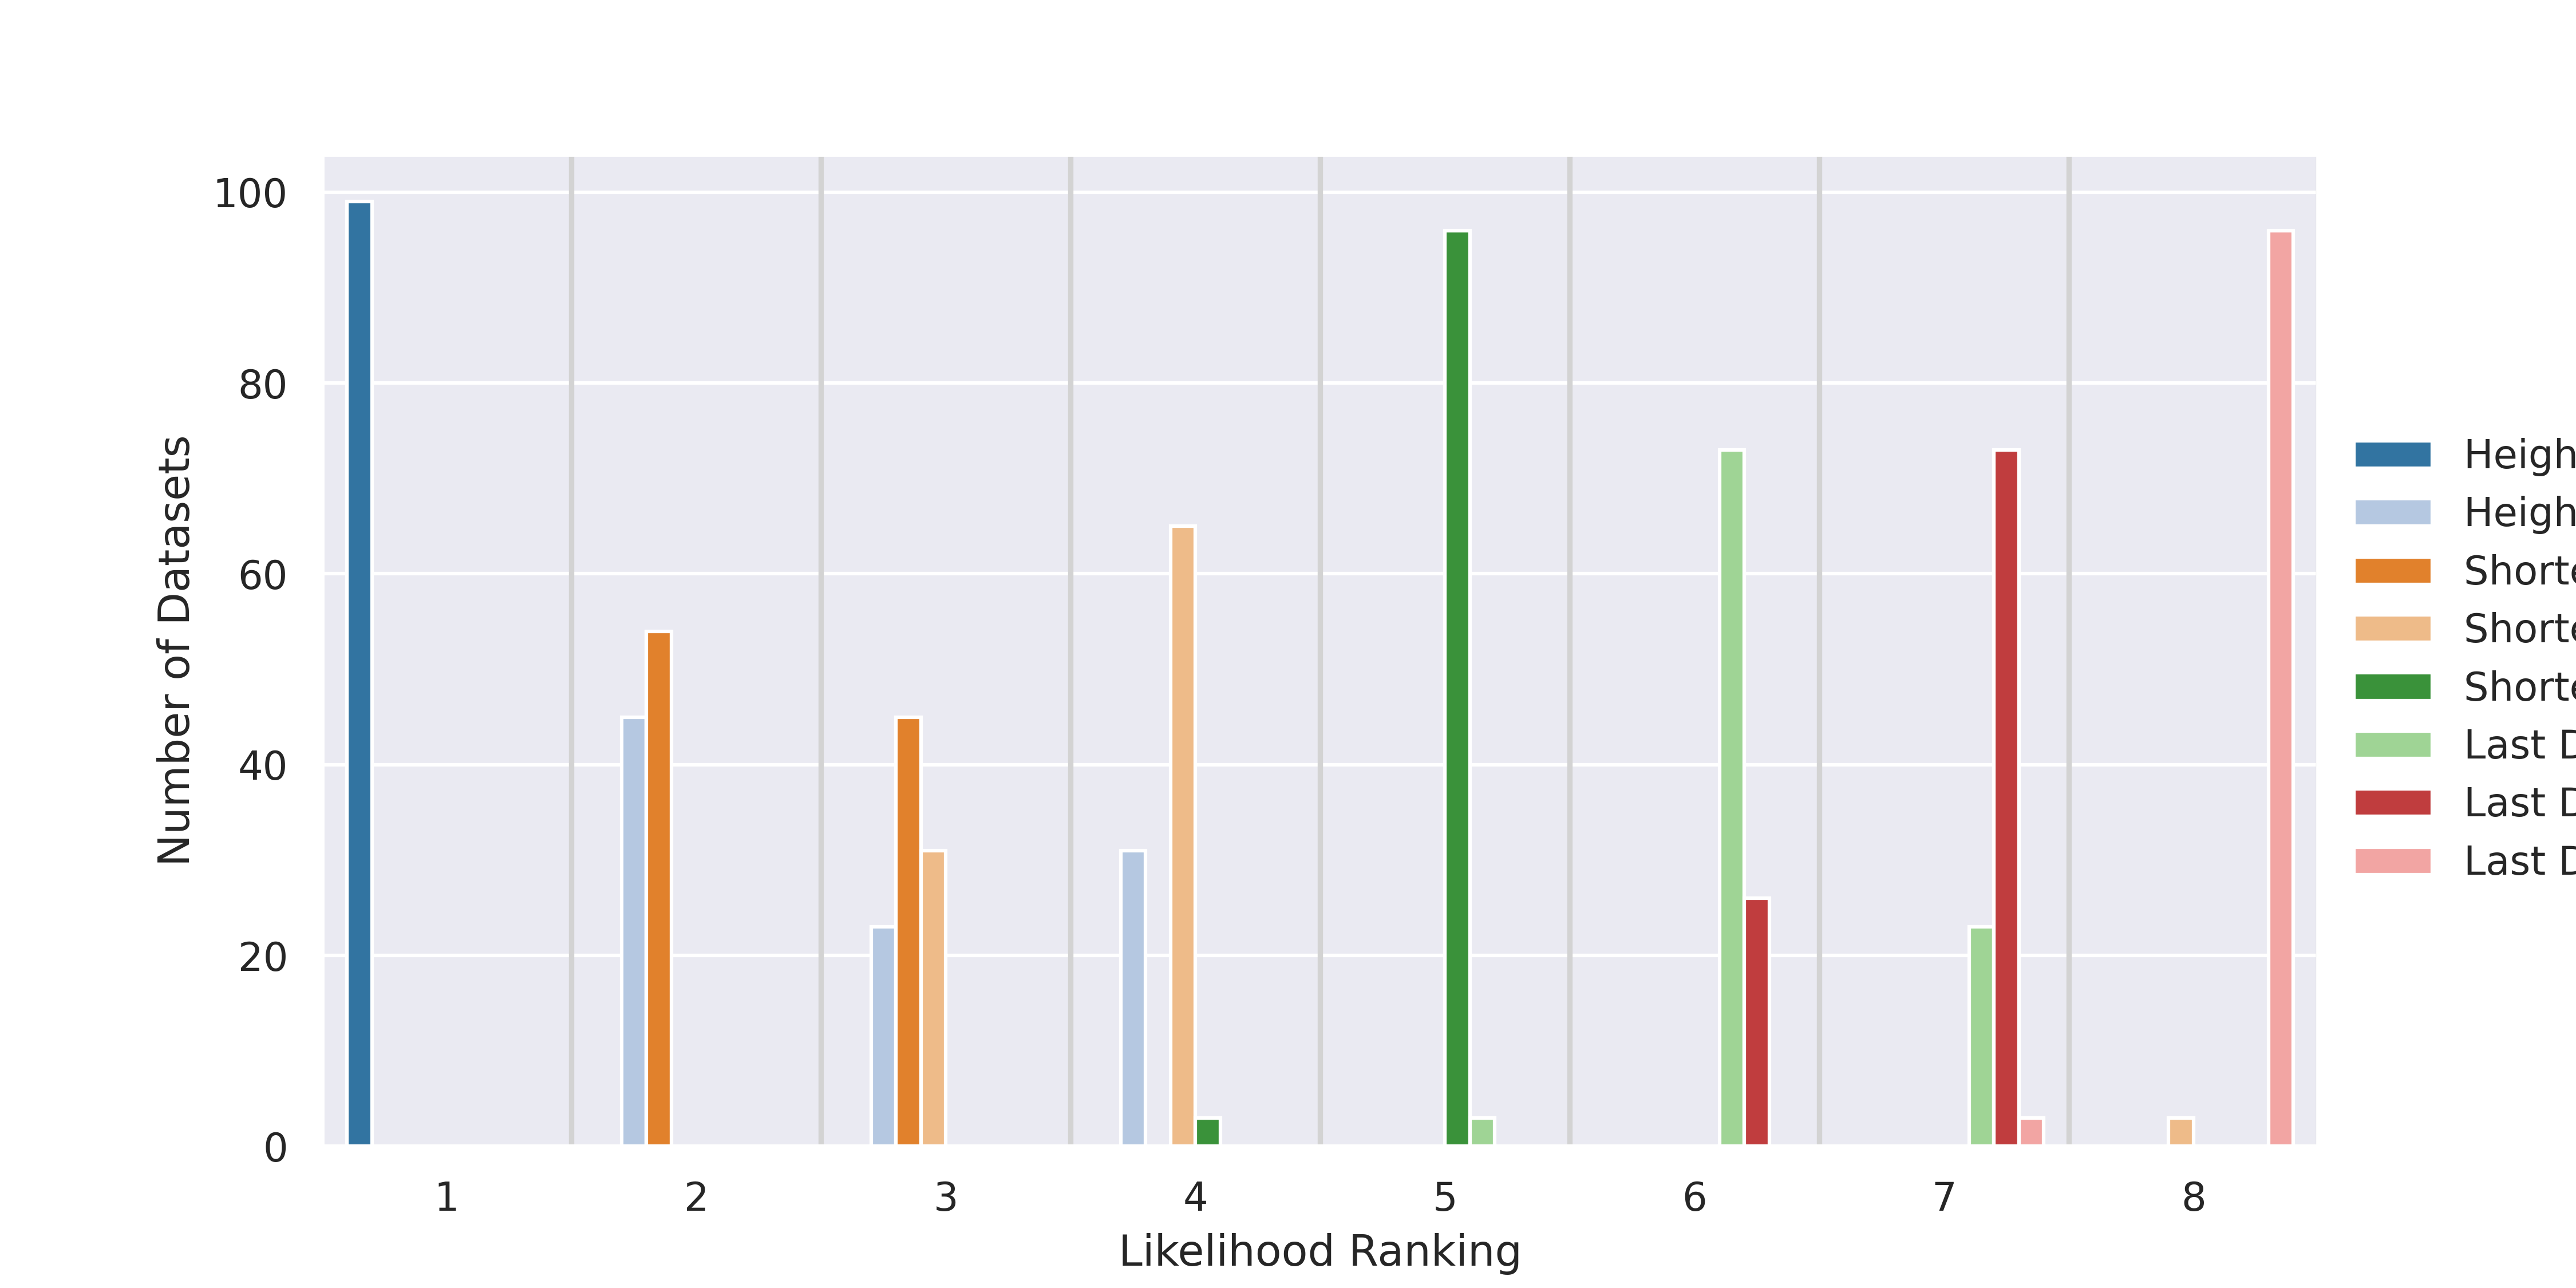
\includegraphics[width=\textwidth]{figures/yule-400-ccd1-likelihood-ranking.png}
		\subcaption{Yule-400}
	\end{subfigure}
	\begin{subfigure}[b]{0.45\textwidth}
		\centering
		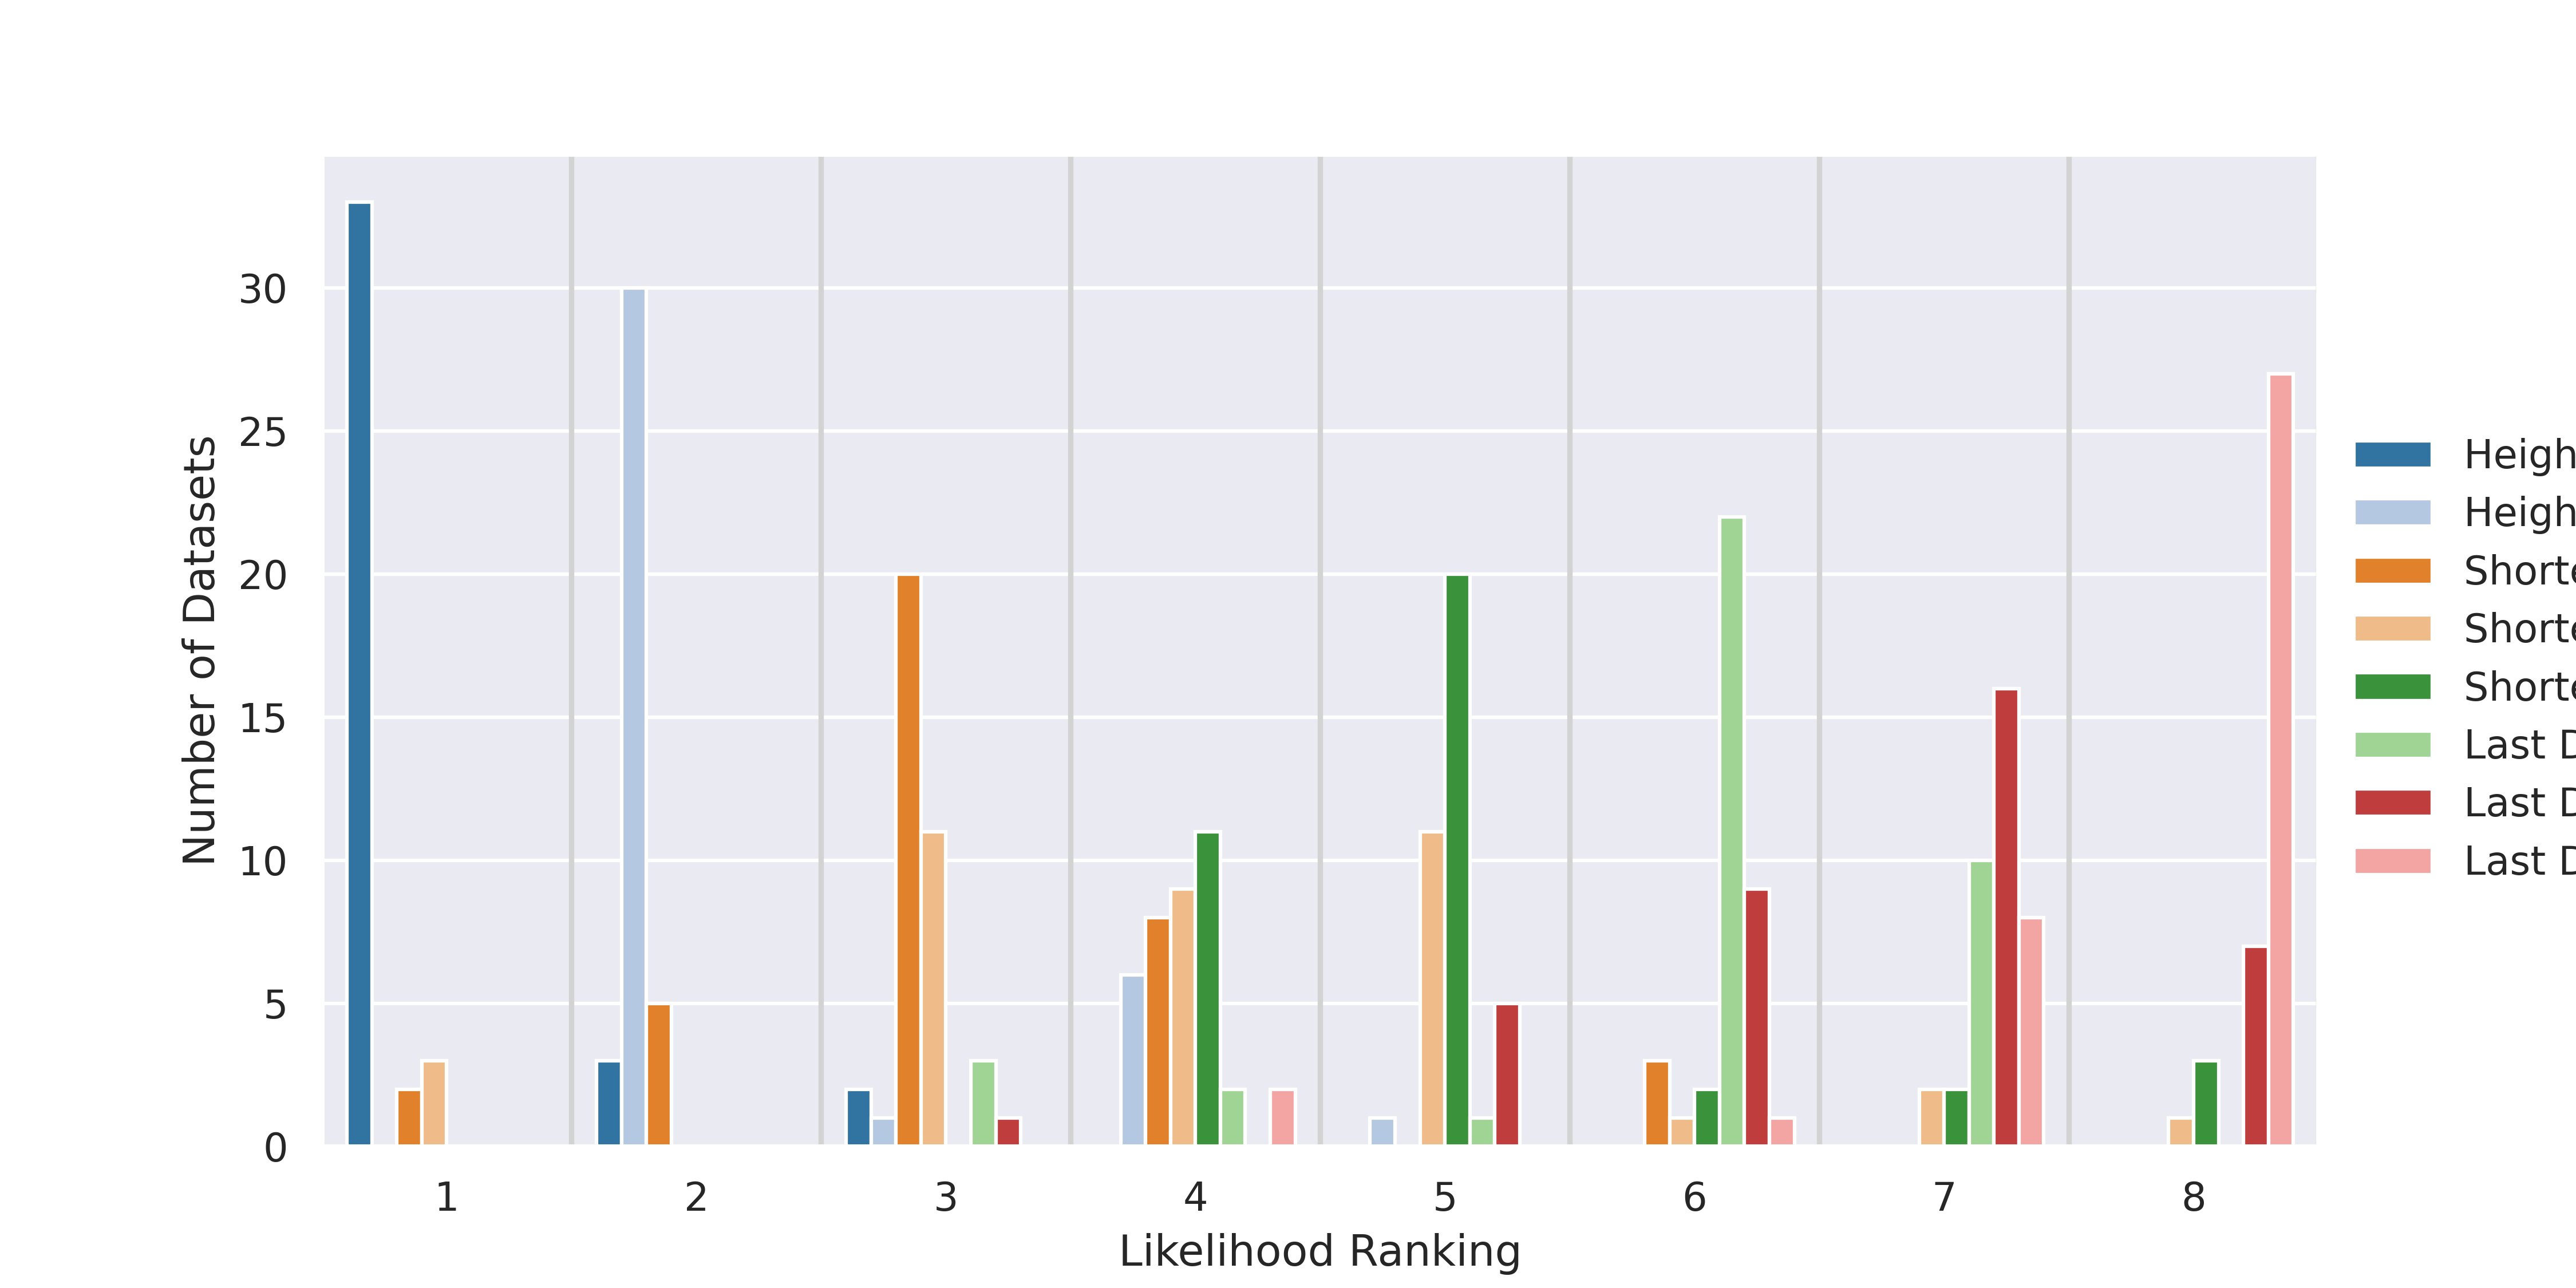
\includegraphics[width=\textwidth]{figures/bio-ccd1-likelihood-ranking.png}
		\subcaption{Real-world datasets}
	\end{subfigure}
	
	\label{fig:data-likelihood-ranking}
\end{figure}

\subsection*{Goodness-of-fit}

To assess the goodness-of-fit, we first examine the Cramér-von Mises criterion of the credible-region plots. The smaller the criterion, the smaller the deviation to the $x=y$ line in the credible-region plots. The smaller the deviation, the better the approximate distribution captures the smallest $\gamma$-credible region for different values of $\gamma$. Figure \ref{fig:cramer-von-mises} shows the Cramér-von Mises criterion for the various distributions and datasets, while figure \ref{fig:cramer-von-mises-ranking} shows how often a specific method ranks at a particular position when compared to the other methods. Interestingly, the ranking observed for the data likelihood is also apparent in the ranking of the Cramér-von Mises criterion for the real-world datasets: The height ratio embeddings generally perform best, while the shortest branch embedding and the last divergence embedding shows no clear tendency. On the other hand, the Cramér-von Mises criterion for the simulated Yule datasets tells a different story, with the height ratio embedding generally showing the highest deviation to the $x=y$ line. (Why is that?)

\begin{figure}
	\caption{The Cramér-von Mises criterion for the different distributions and datasets. (The lower the better.)}
	
	\centering
	\begin{subfigure}[b]{0.45\textwidth}
		\centering
		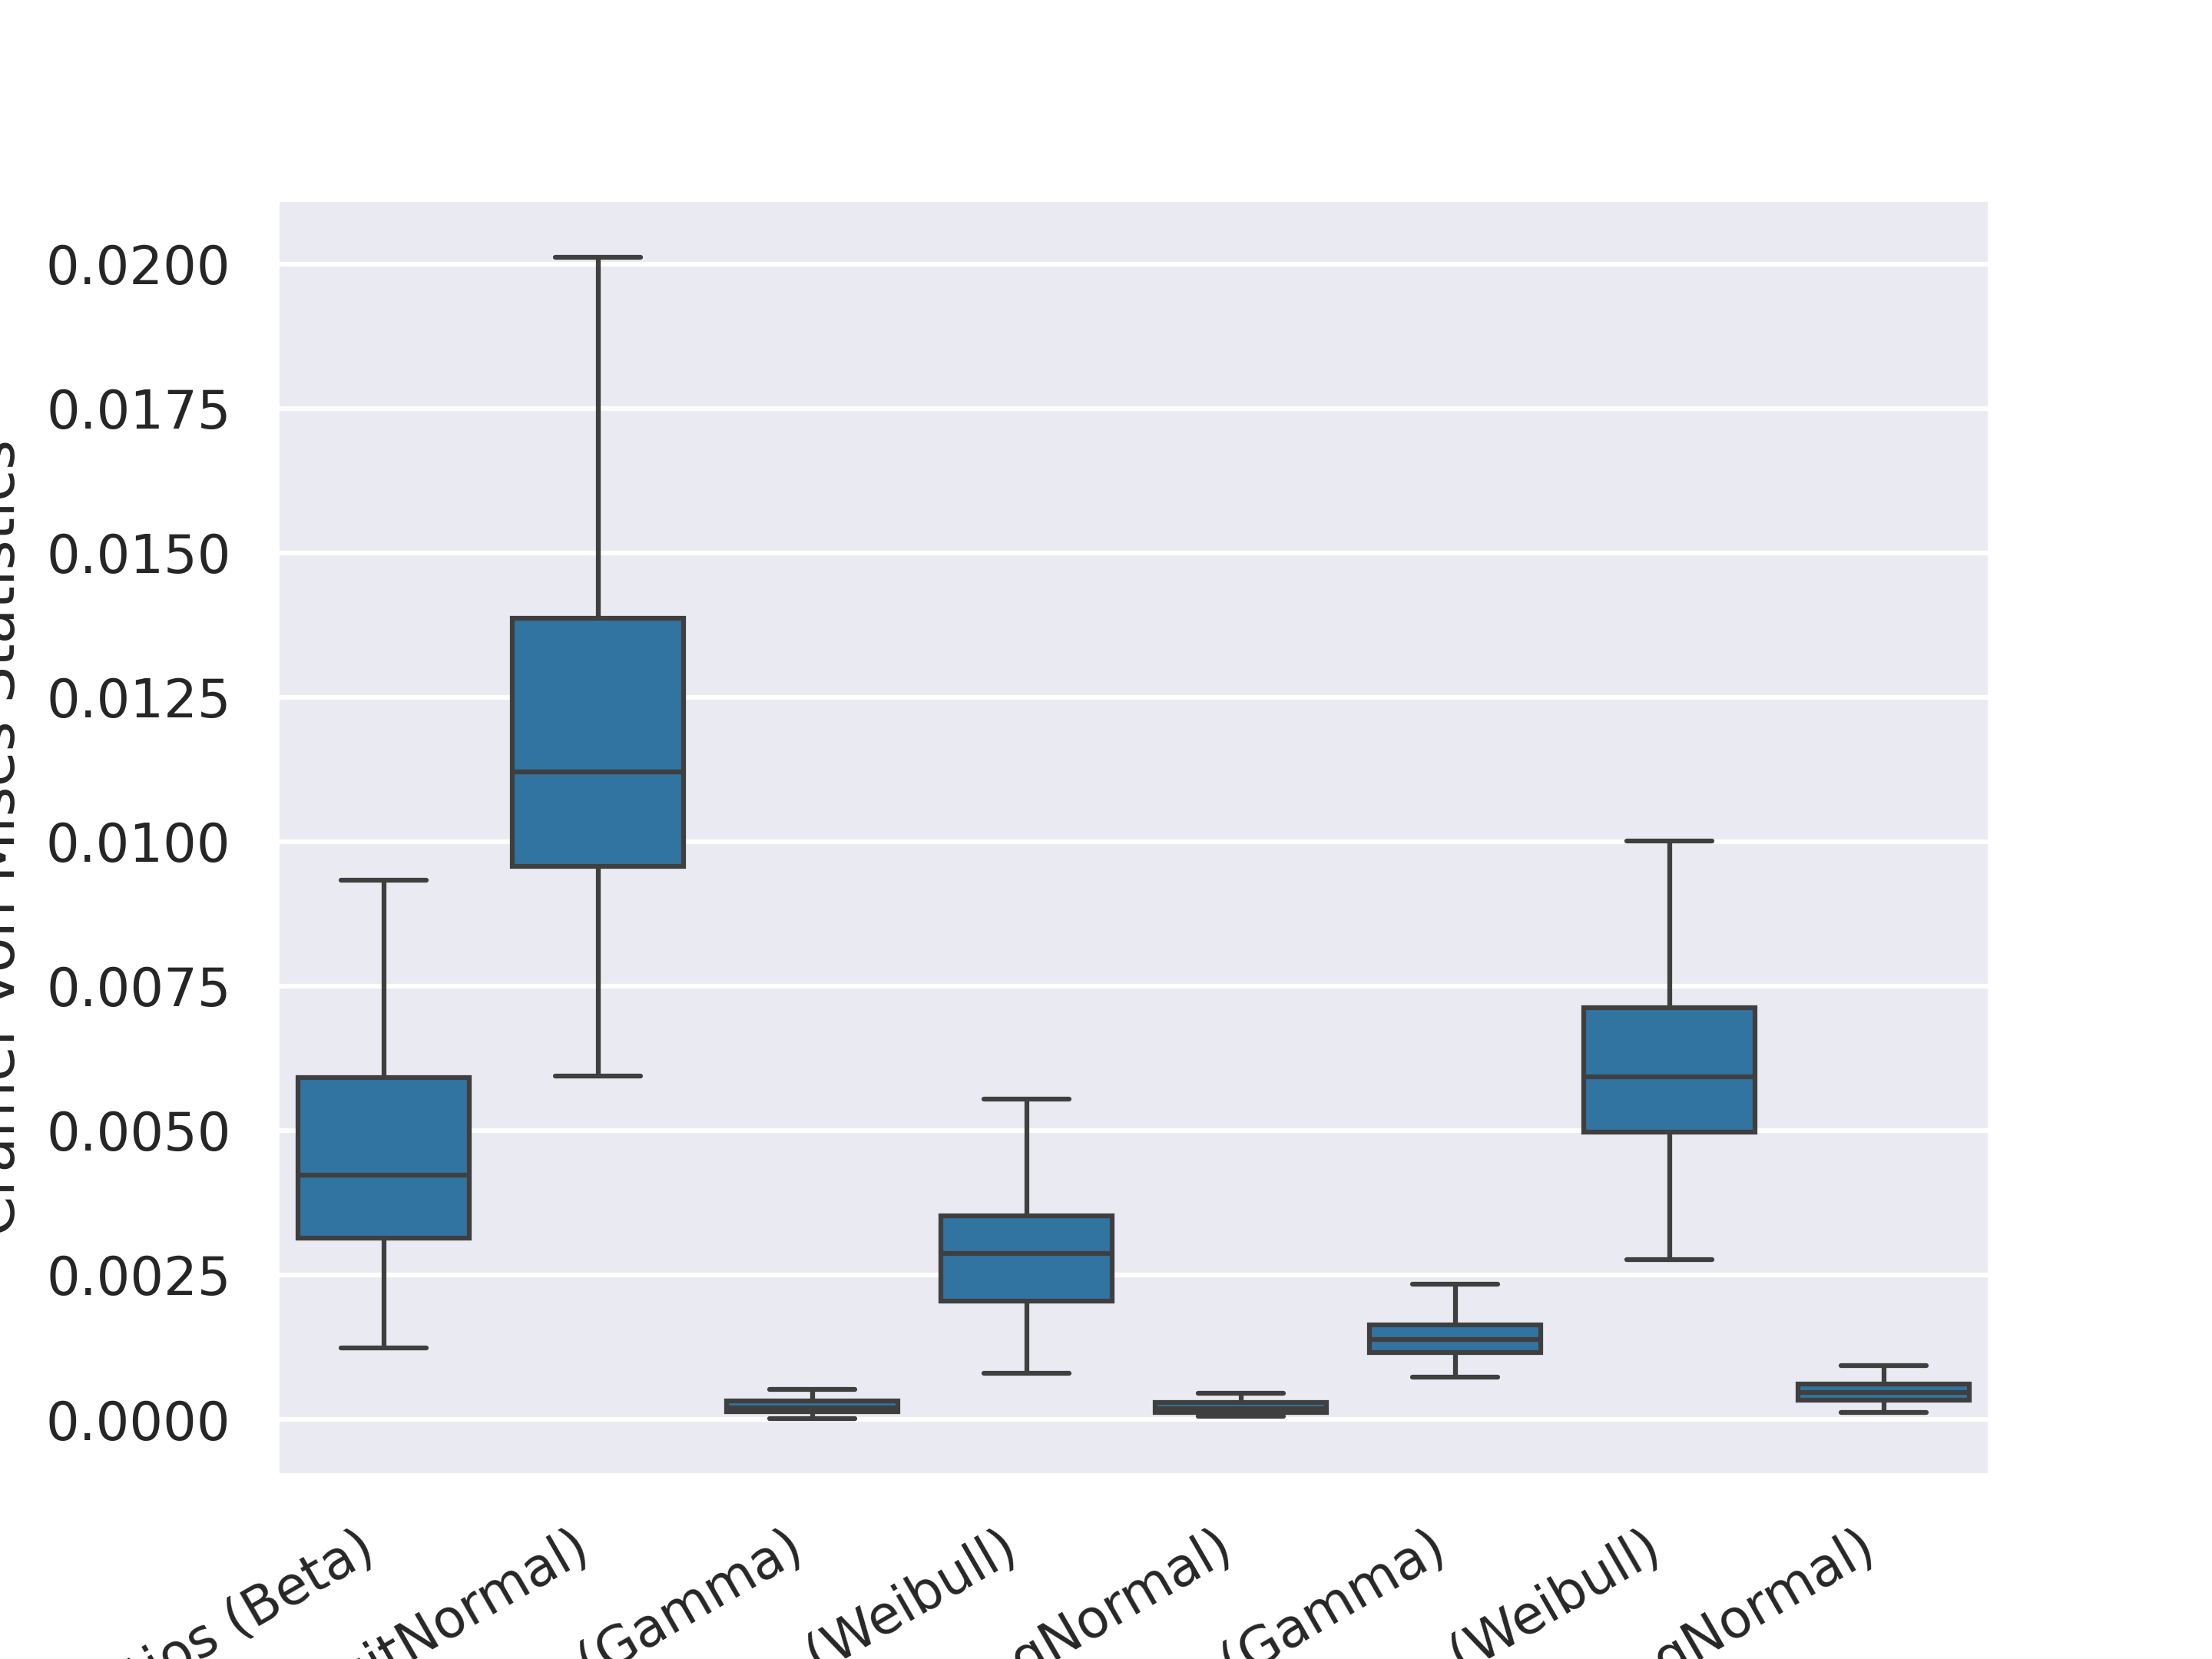
\includegraphics[width=\textwidth]{figures/yule-100-ccd1-cvm.png}
		\subcaption{Yule-100}
	\end{subfigure}
	\begin{subfigure}[b]{0.45\textwidth}
		\centering
		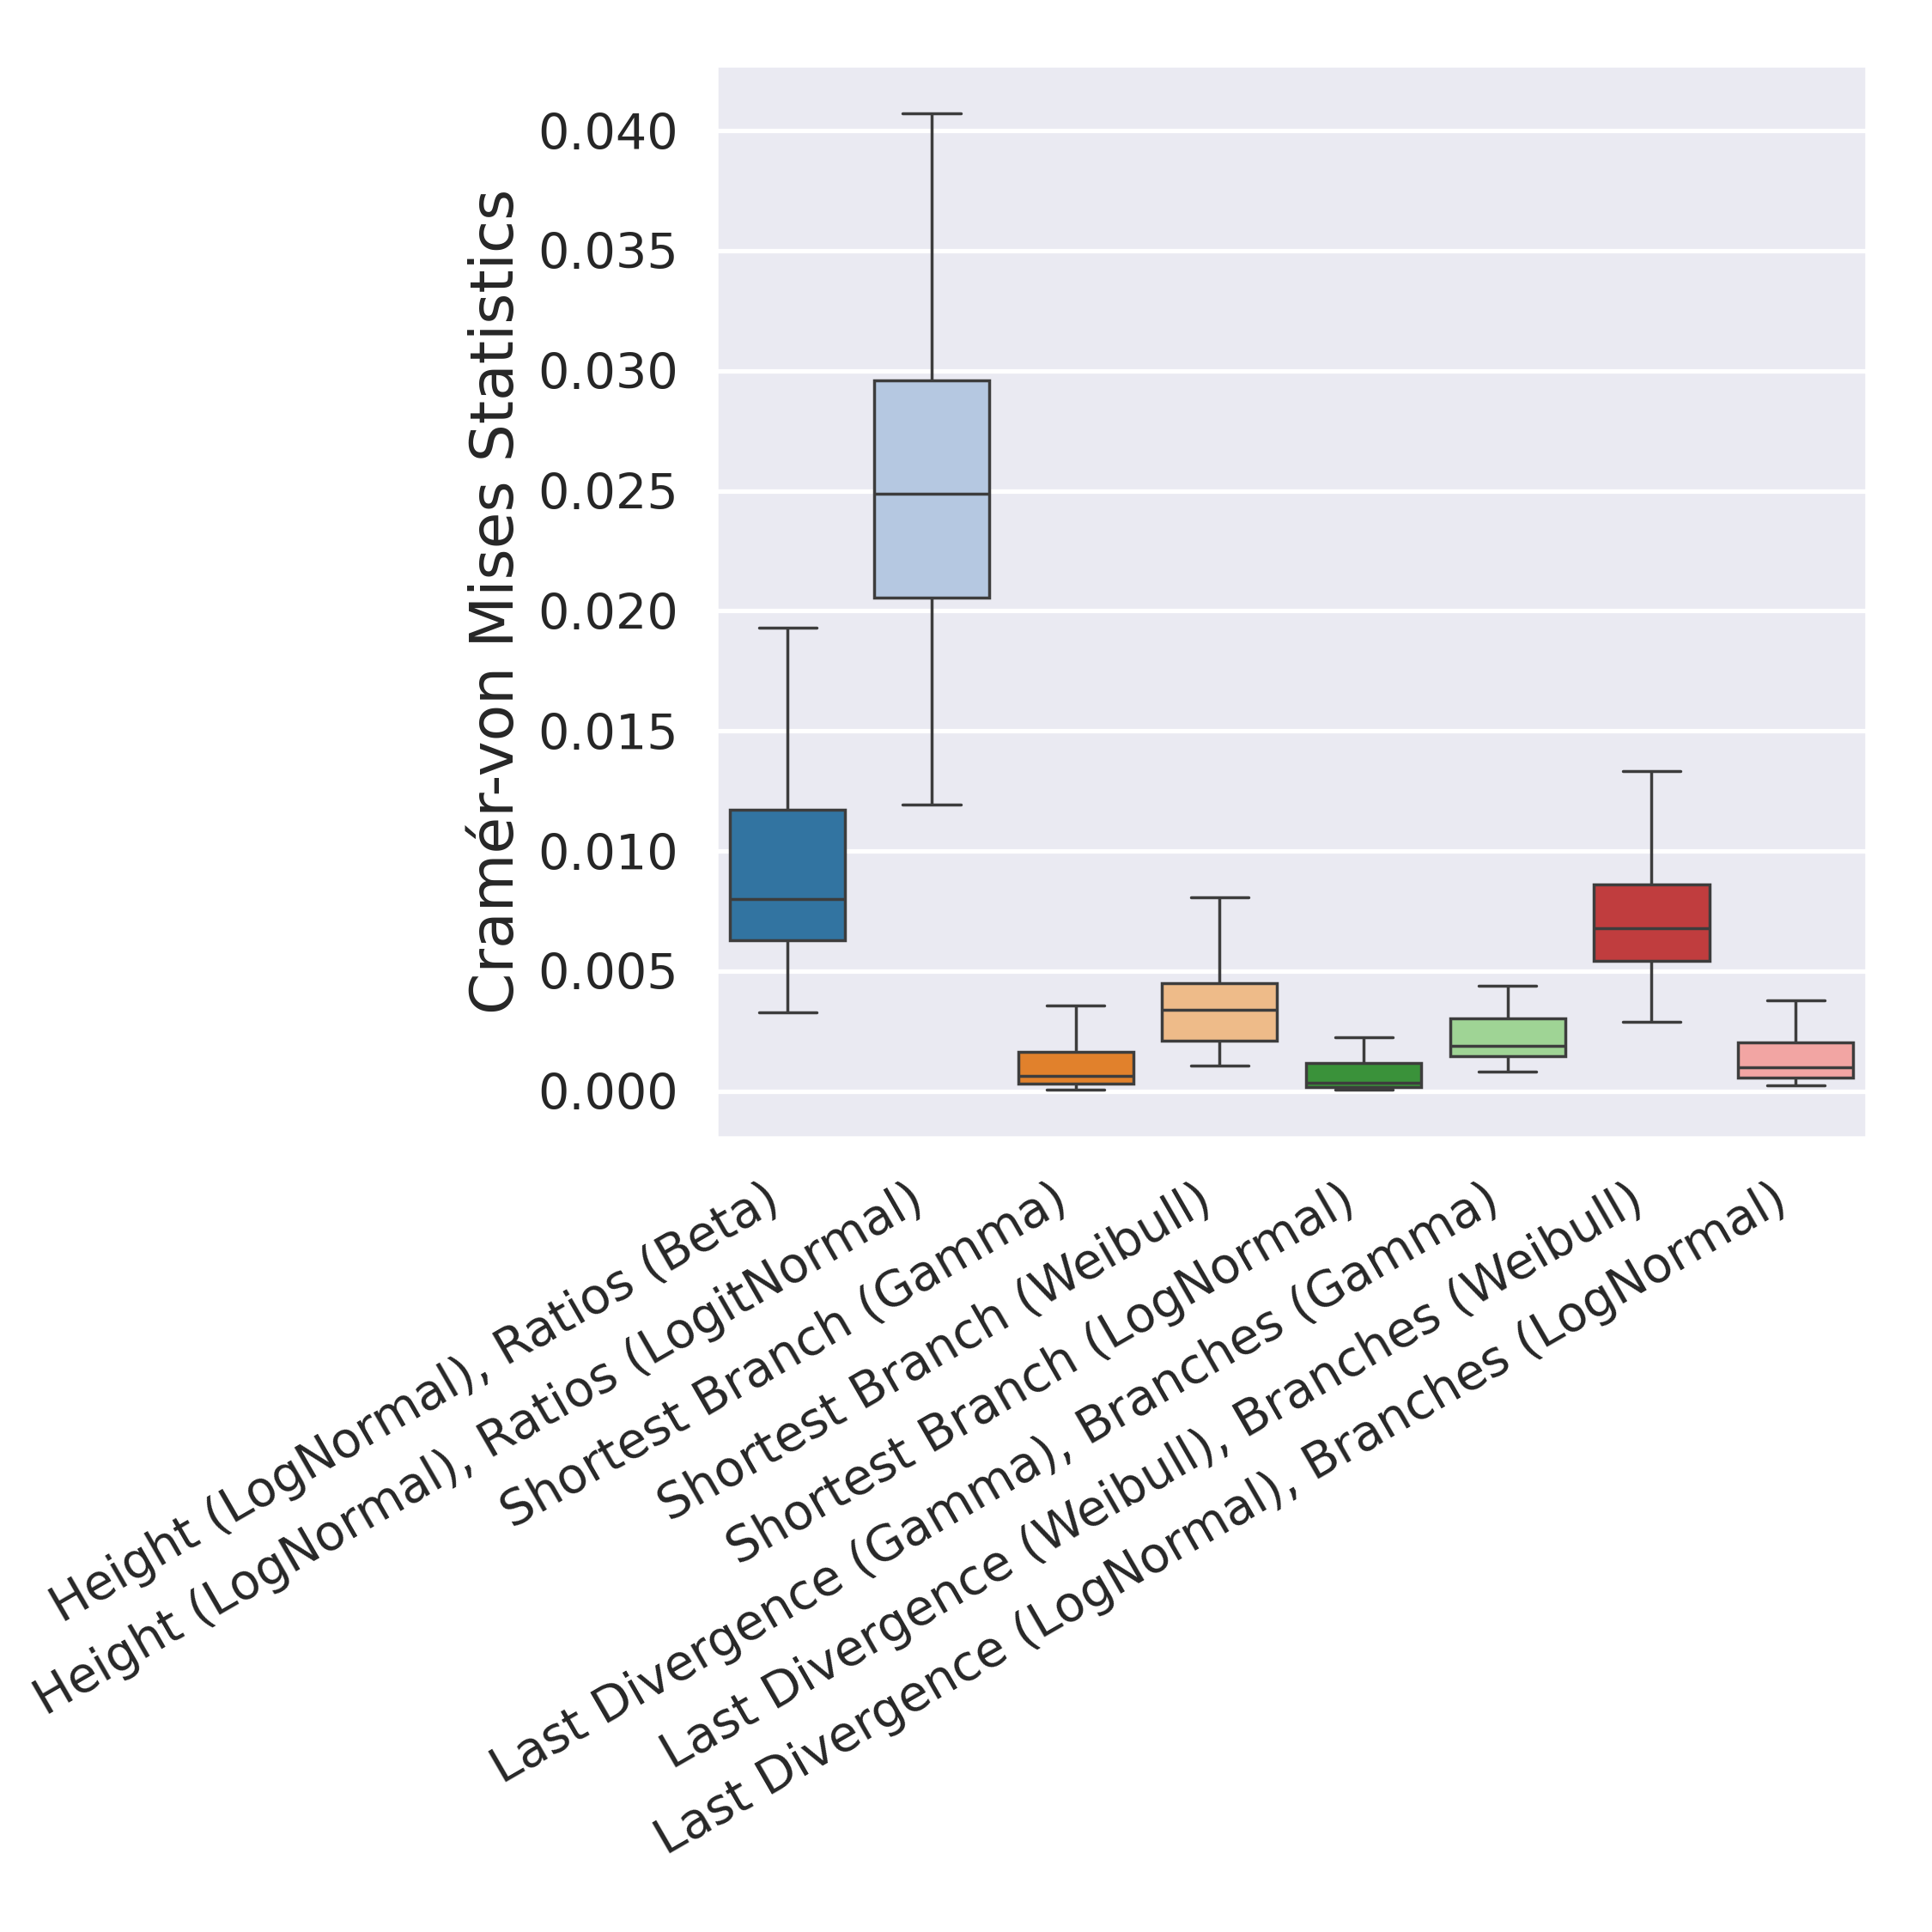
\includegraphics[width=\textwidth]{figures/yule-200-ccd1-cvm.png}
		\subcaption{Yule-200}
	\end{subfigure}
	
	\begin{subfigure}[b]{0.45\textwidth}
		\centering
		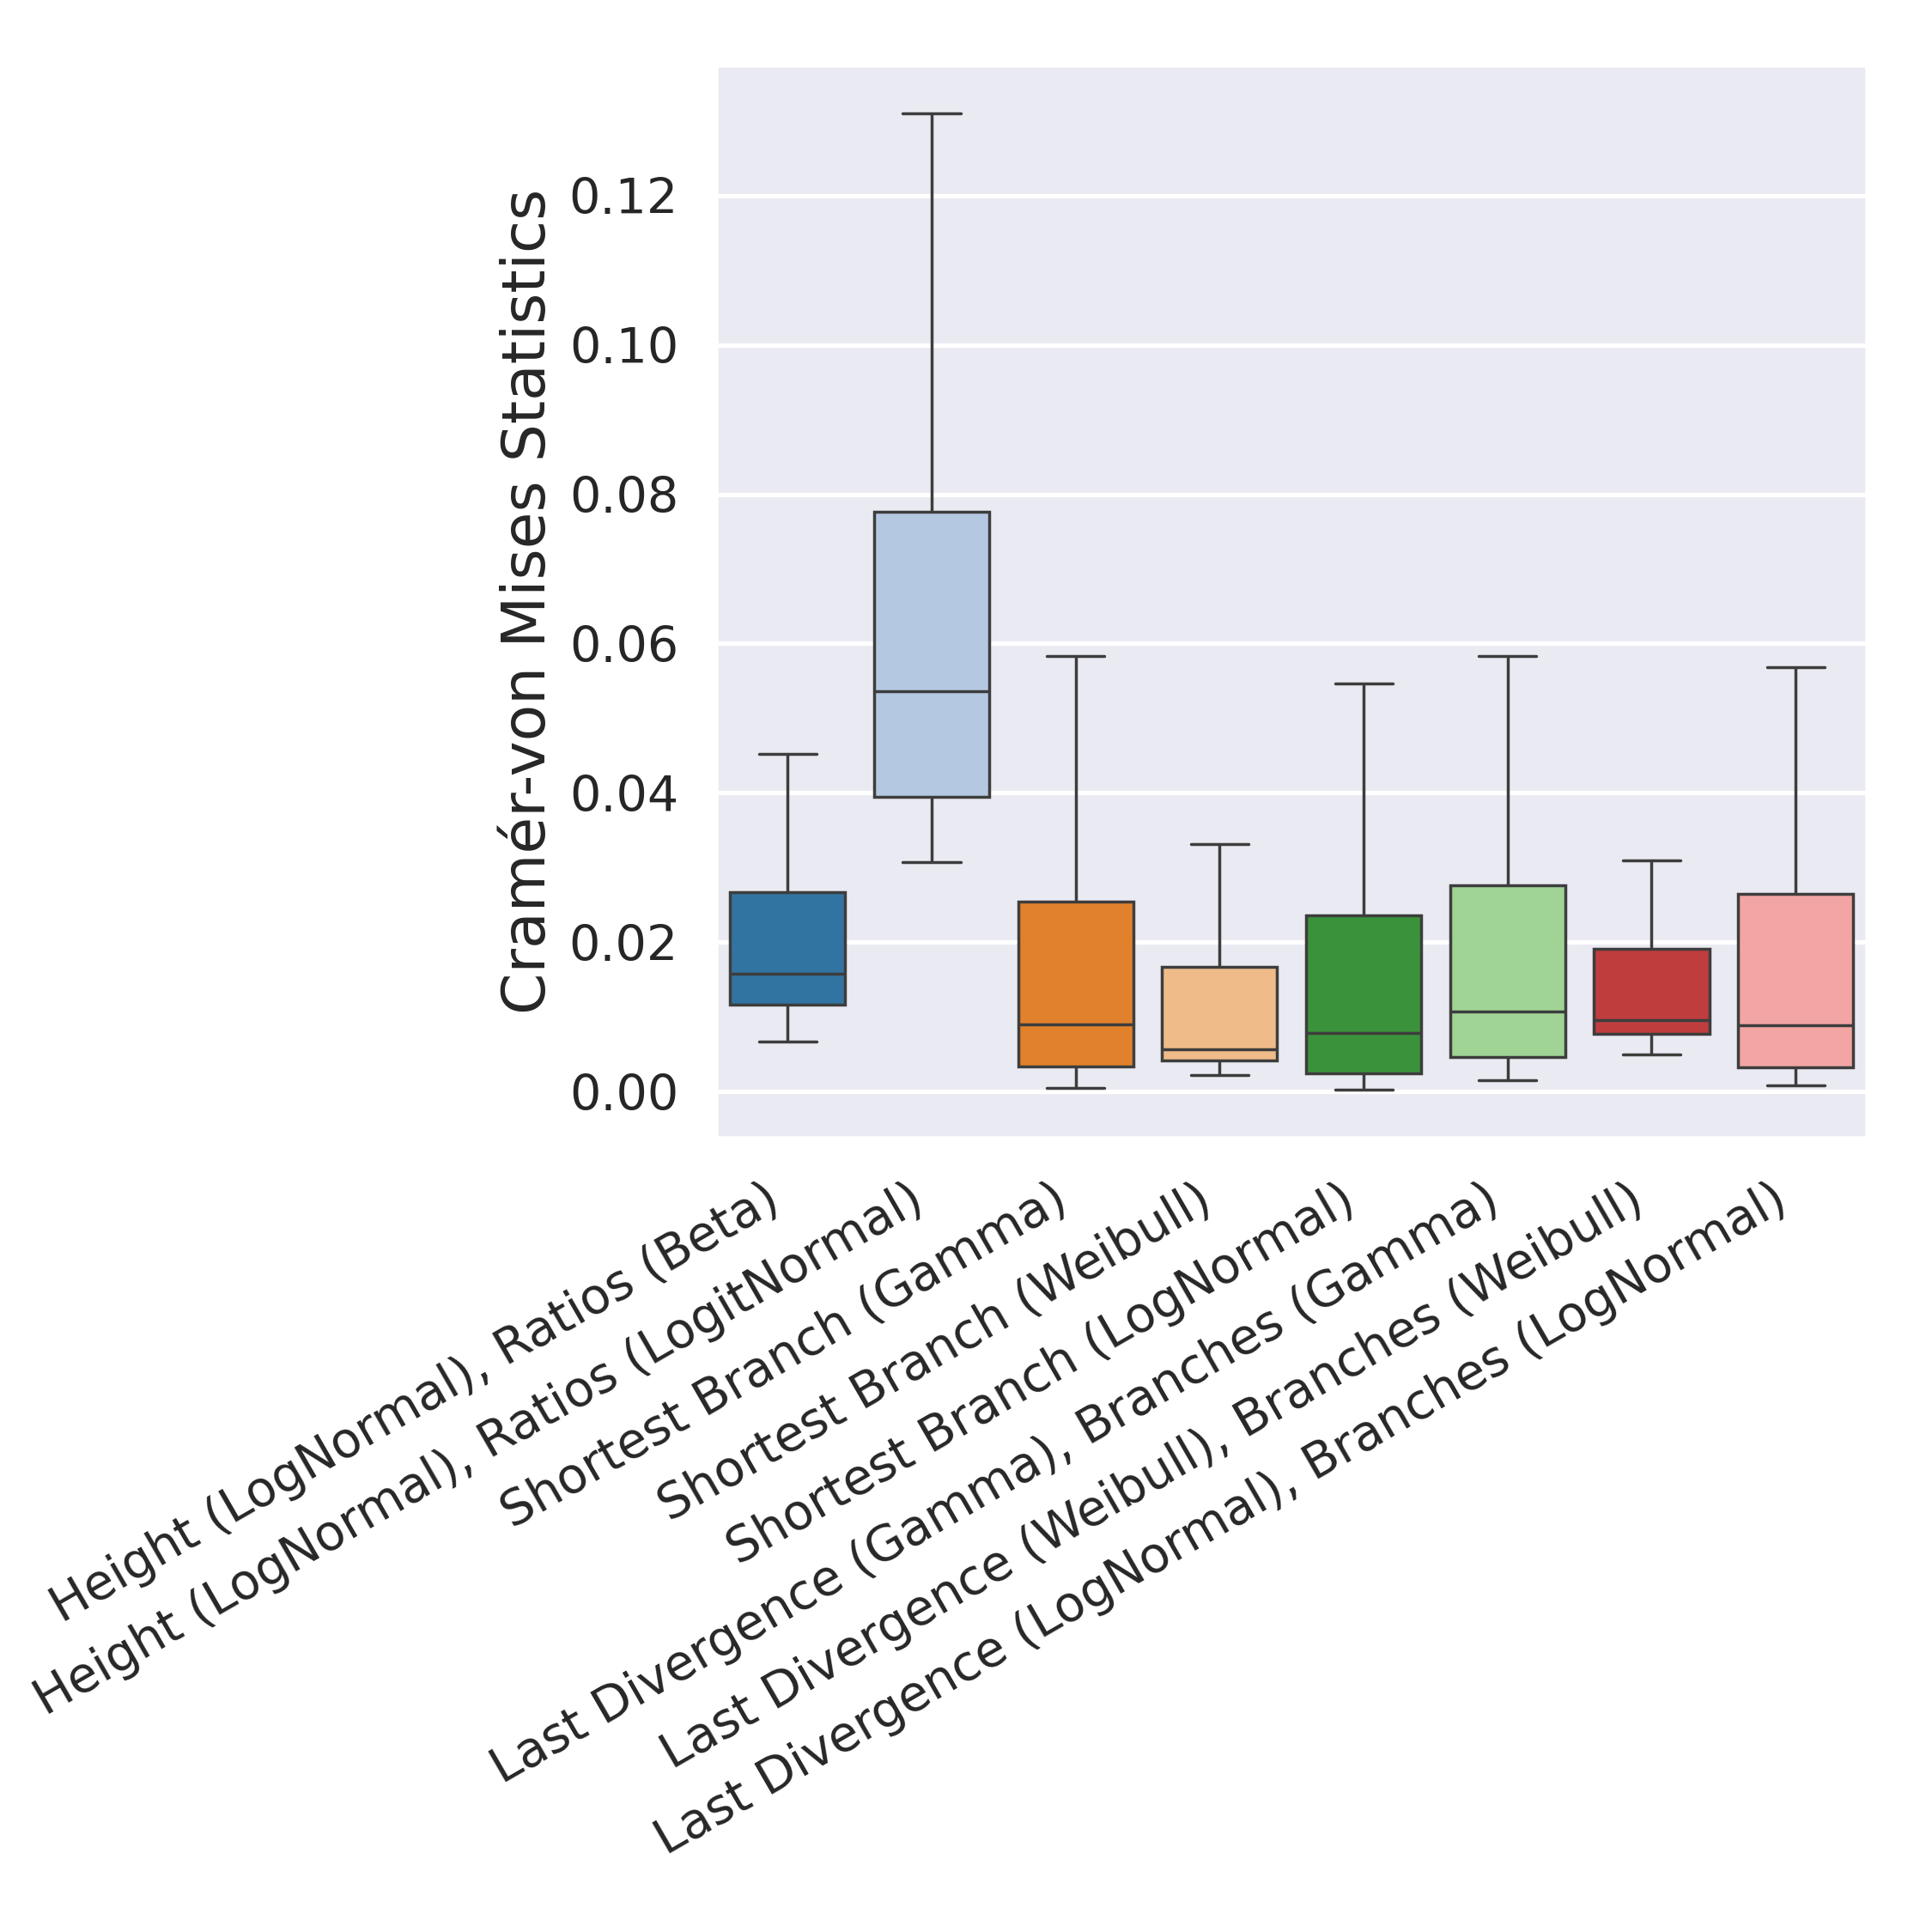
\includegraphics[width=\textwidth]{figures/yule-400-ccd1-cvm.png}
		\subcaption{Yule-400}
	\end{subfigure}
	\begin{subfigure}[b]{0.45\textwidth}
		\centering
		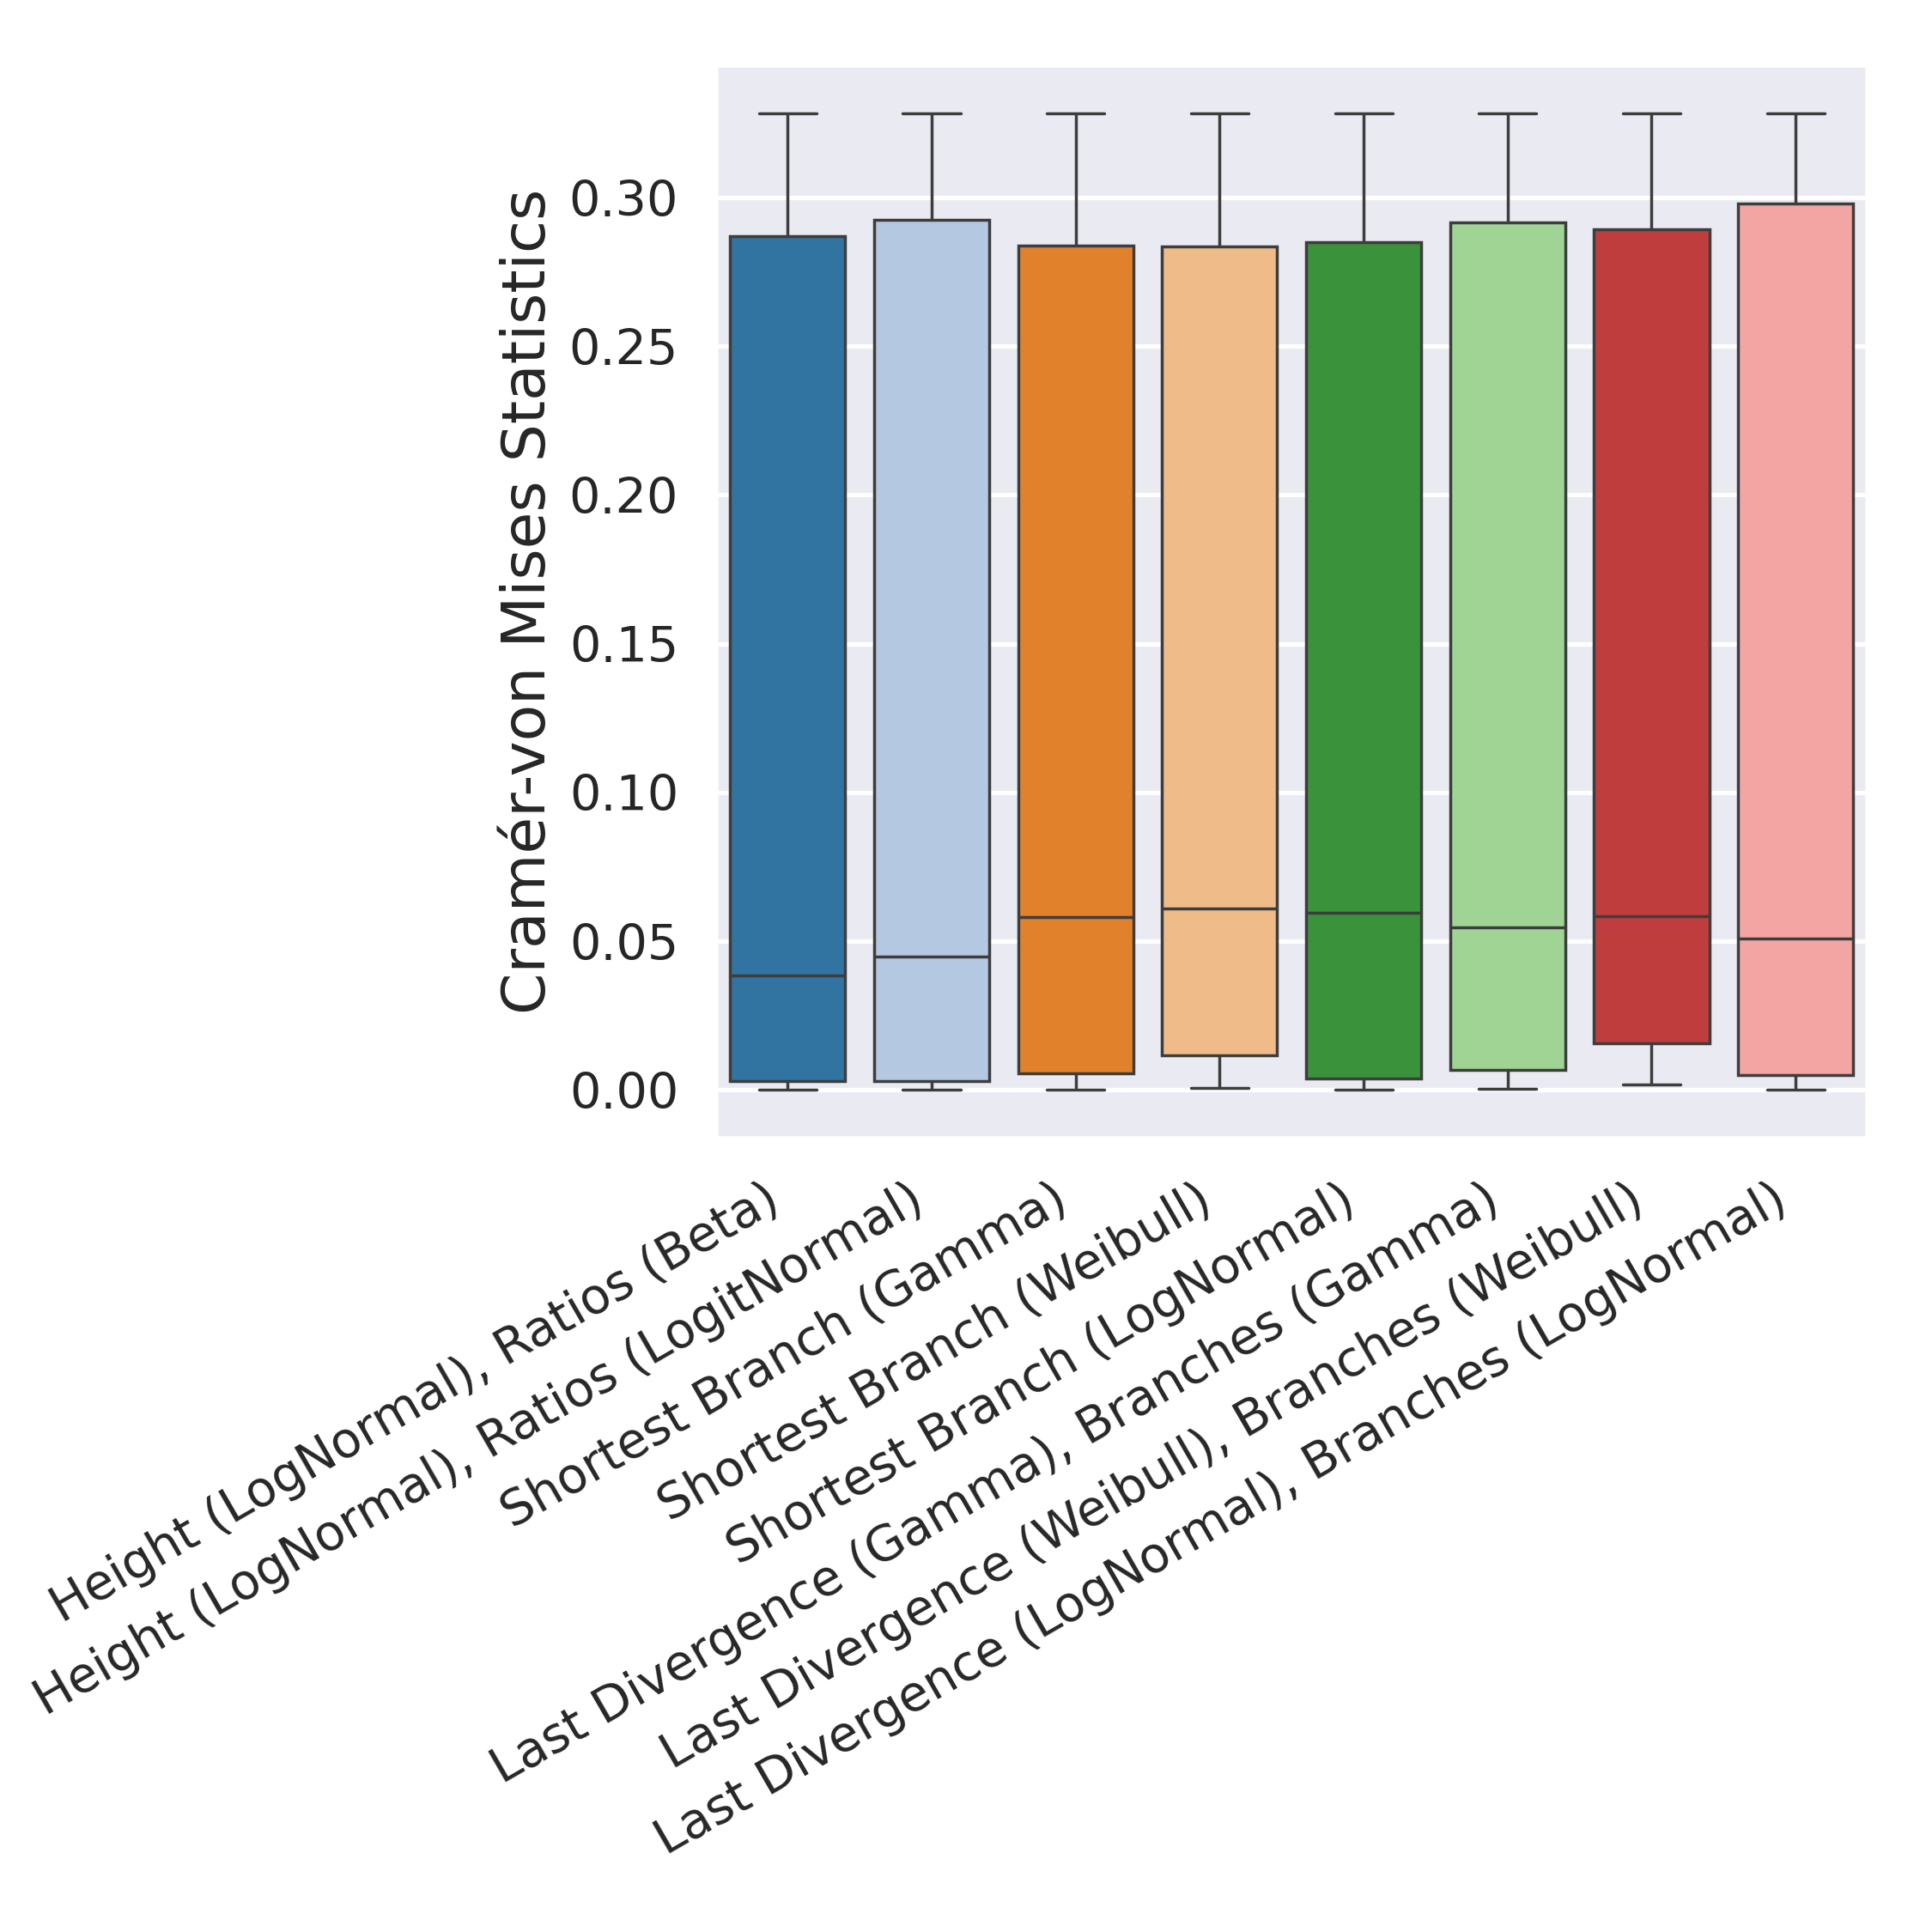
\includegraphics[width=\textwidth]{figures/bio-ccd1-cvm.png}
		\subcaption{Real-world datasets}
	\end{subfigure}
	
	\label{fig:cramer-von-mises}
\end{figure}

\begin{figure}
	\caption{How often a specific method ranks at a certain position when its Cramér-von Mises criterion is compared to the other methods. For example, the height ratio embedding with the beta distribution ranked first for almost all datasets. (The lower the rank the better.)}
	
	\centering
	\begin{subfigure}[b]{0.45\textwidth}
		\centering
		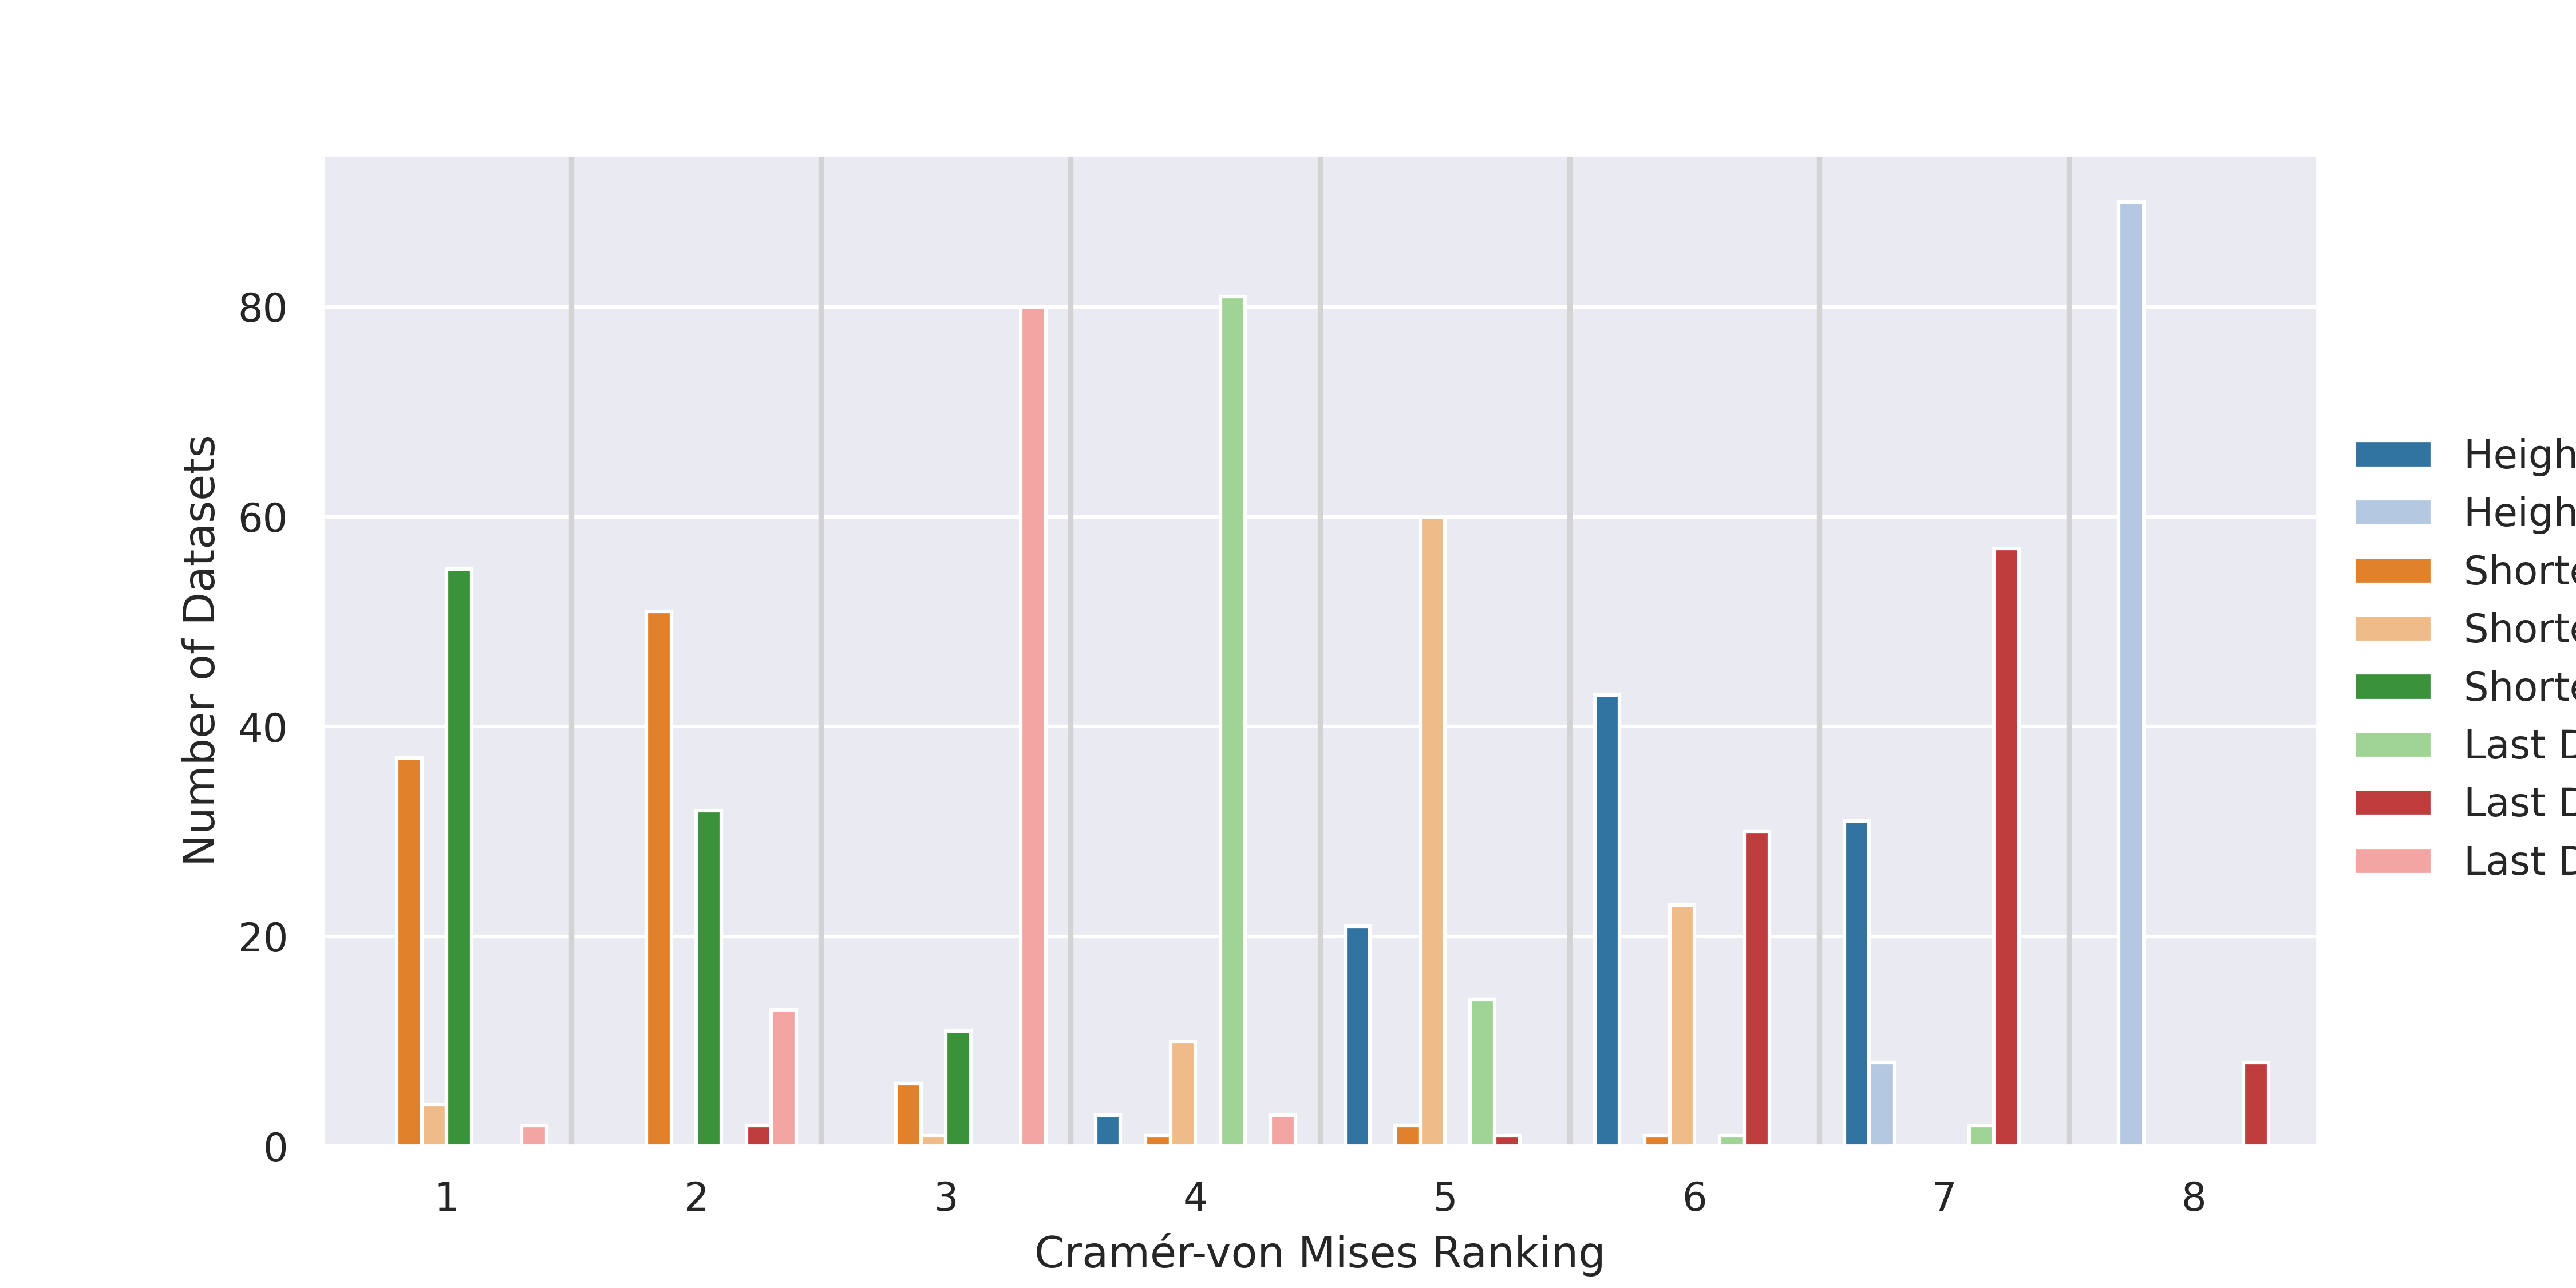
\includegraphics[width=\textwidth]{figures/yule-100-ccd1-cvm-ranking.png}
		\subcaption{Yule-100}
	\end{subfigure}
	\begin{subfigure}[b]{0.45\textwidth}
		\centering
		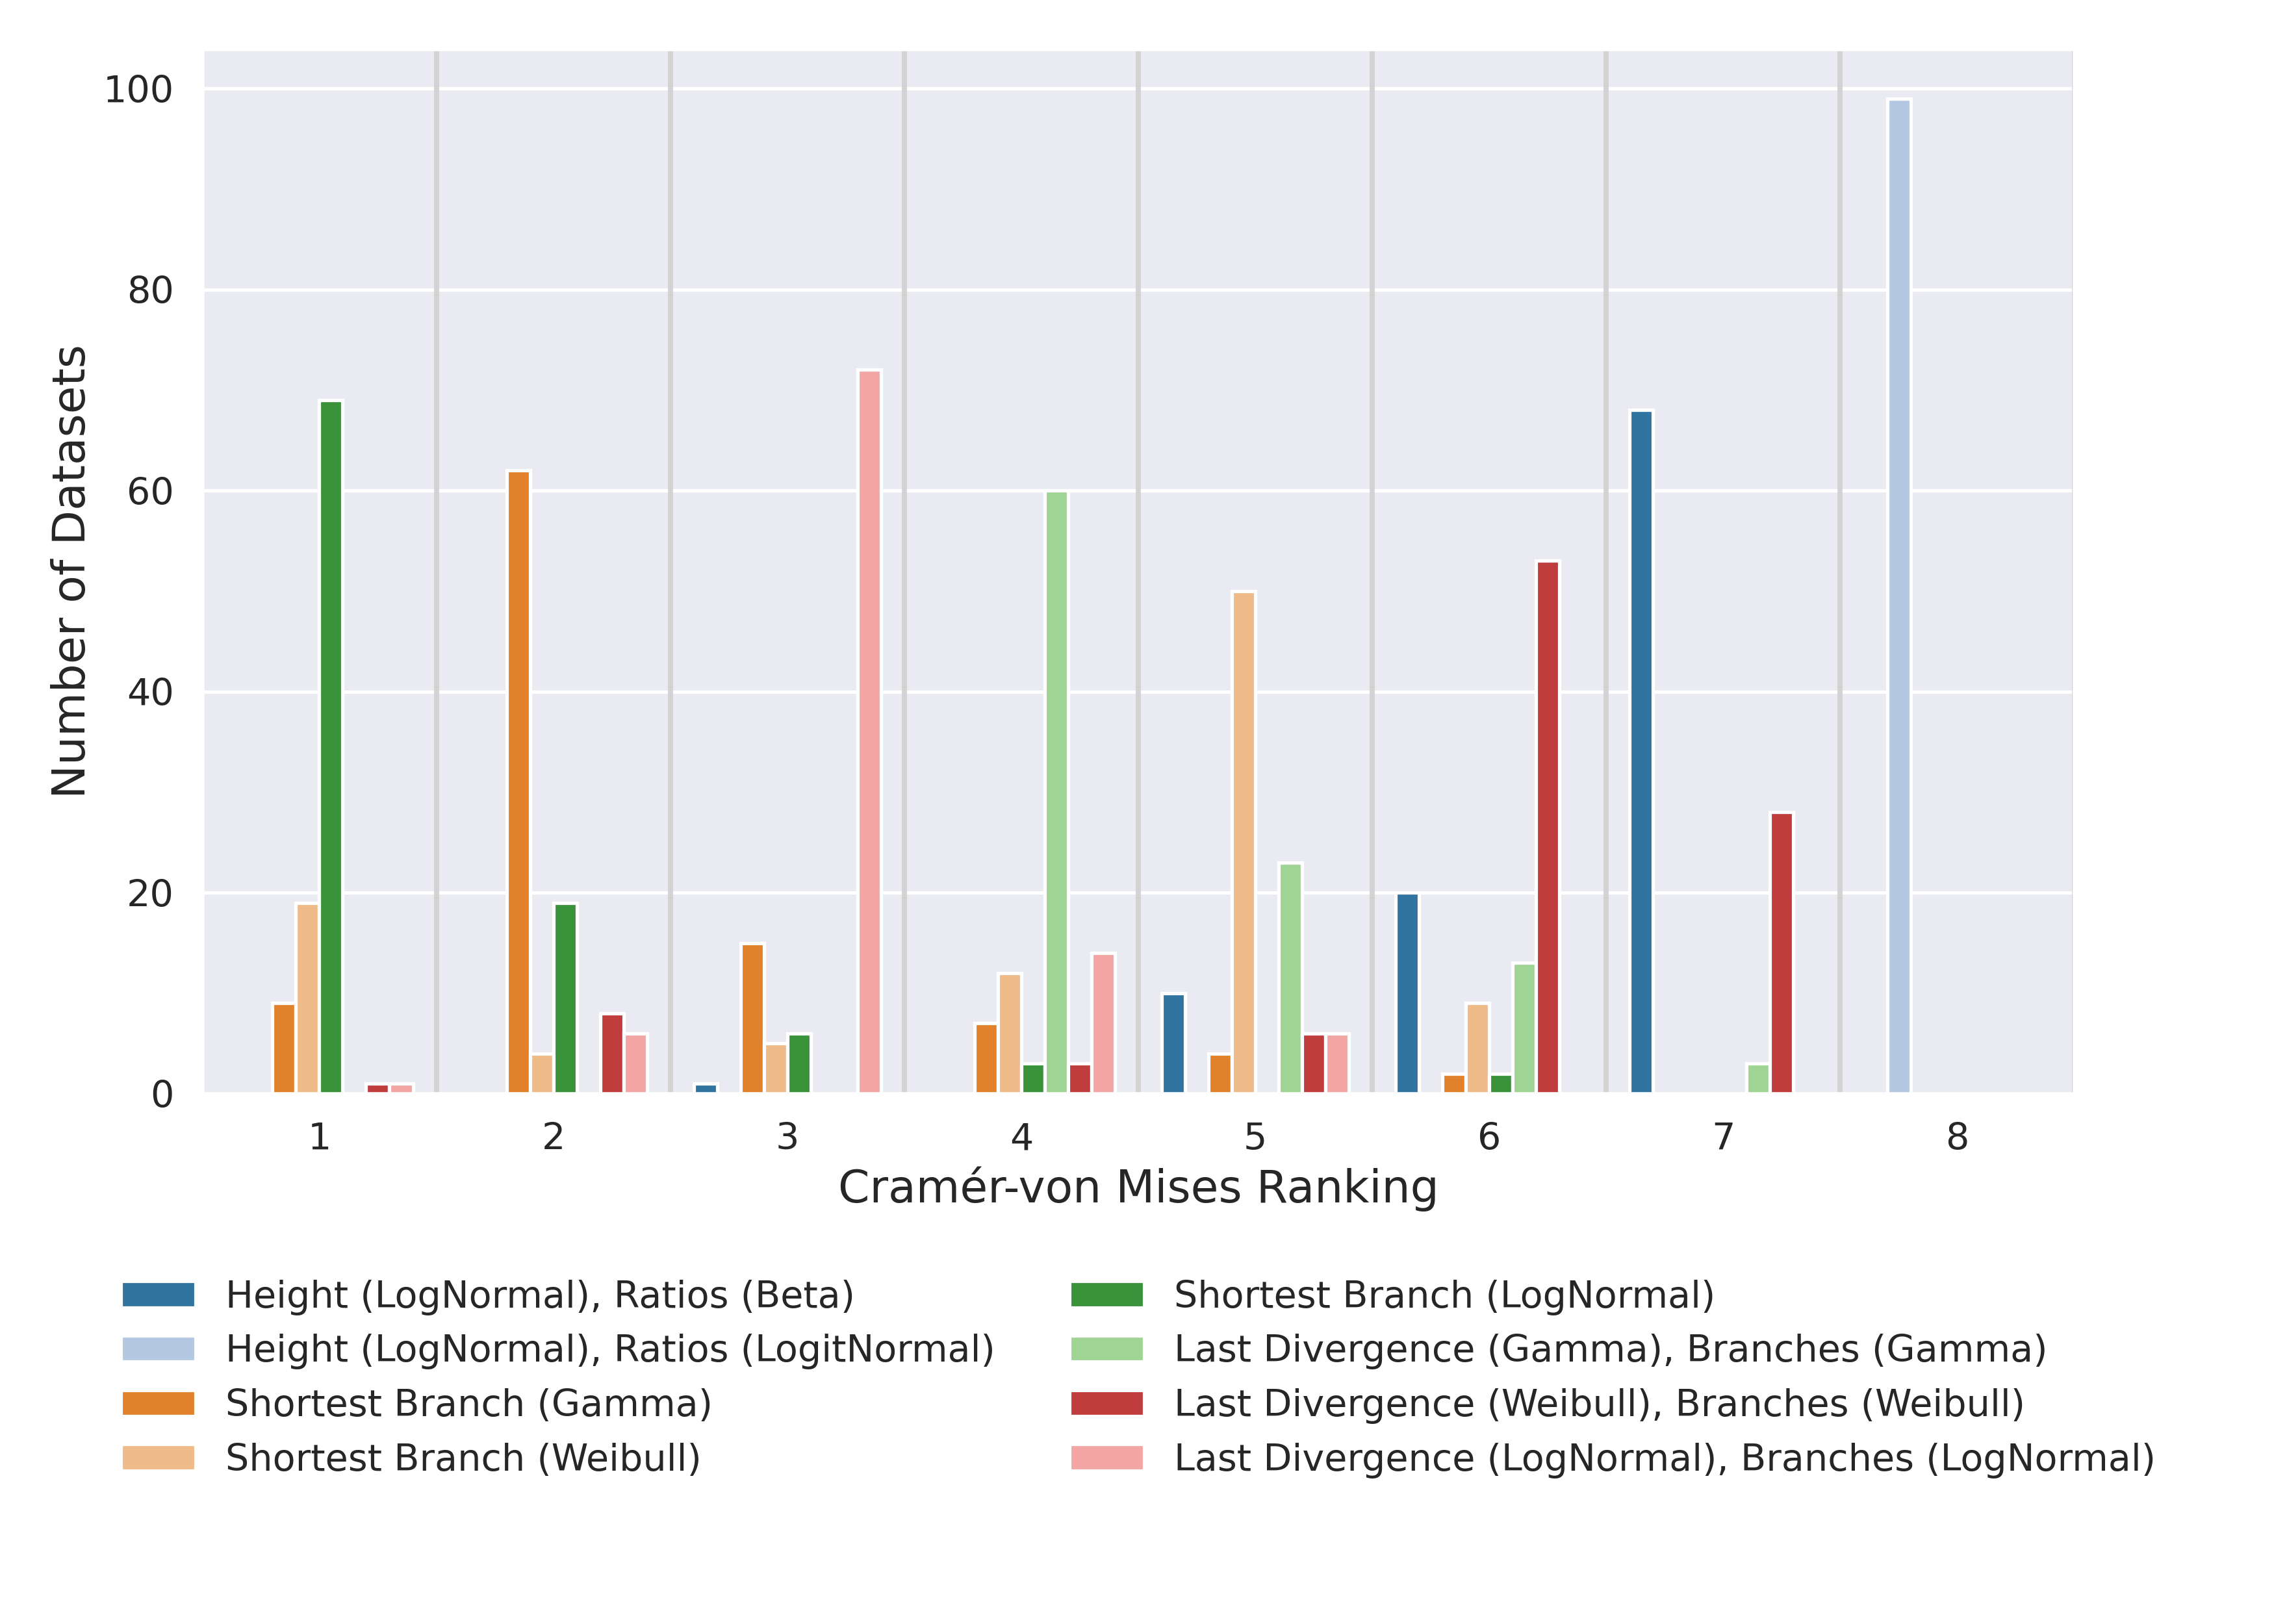
\includegraphics[width=\textwidth]{figures/yule-200-ccd1-cvm-ranking.png}
		\subcaption{Yule-200}
	\end{subfigure}
	
	\begin{subfigure}[b]{0.45\textwidth}
		\centering
		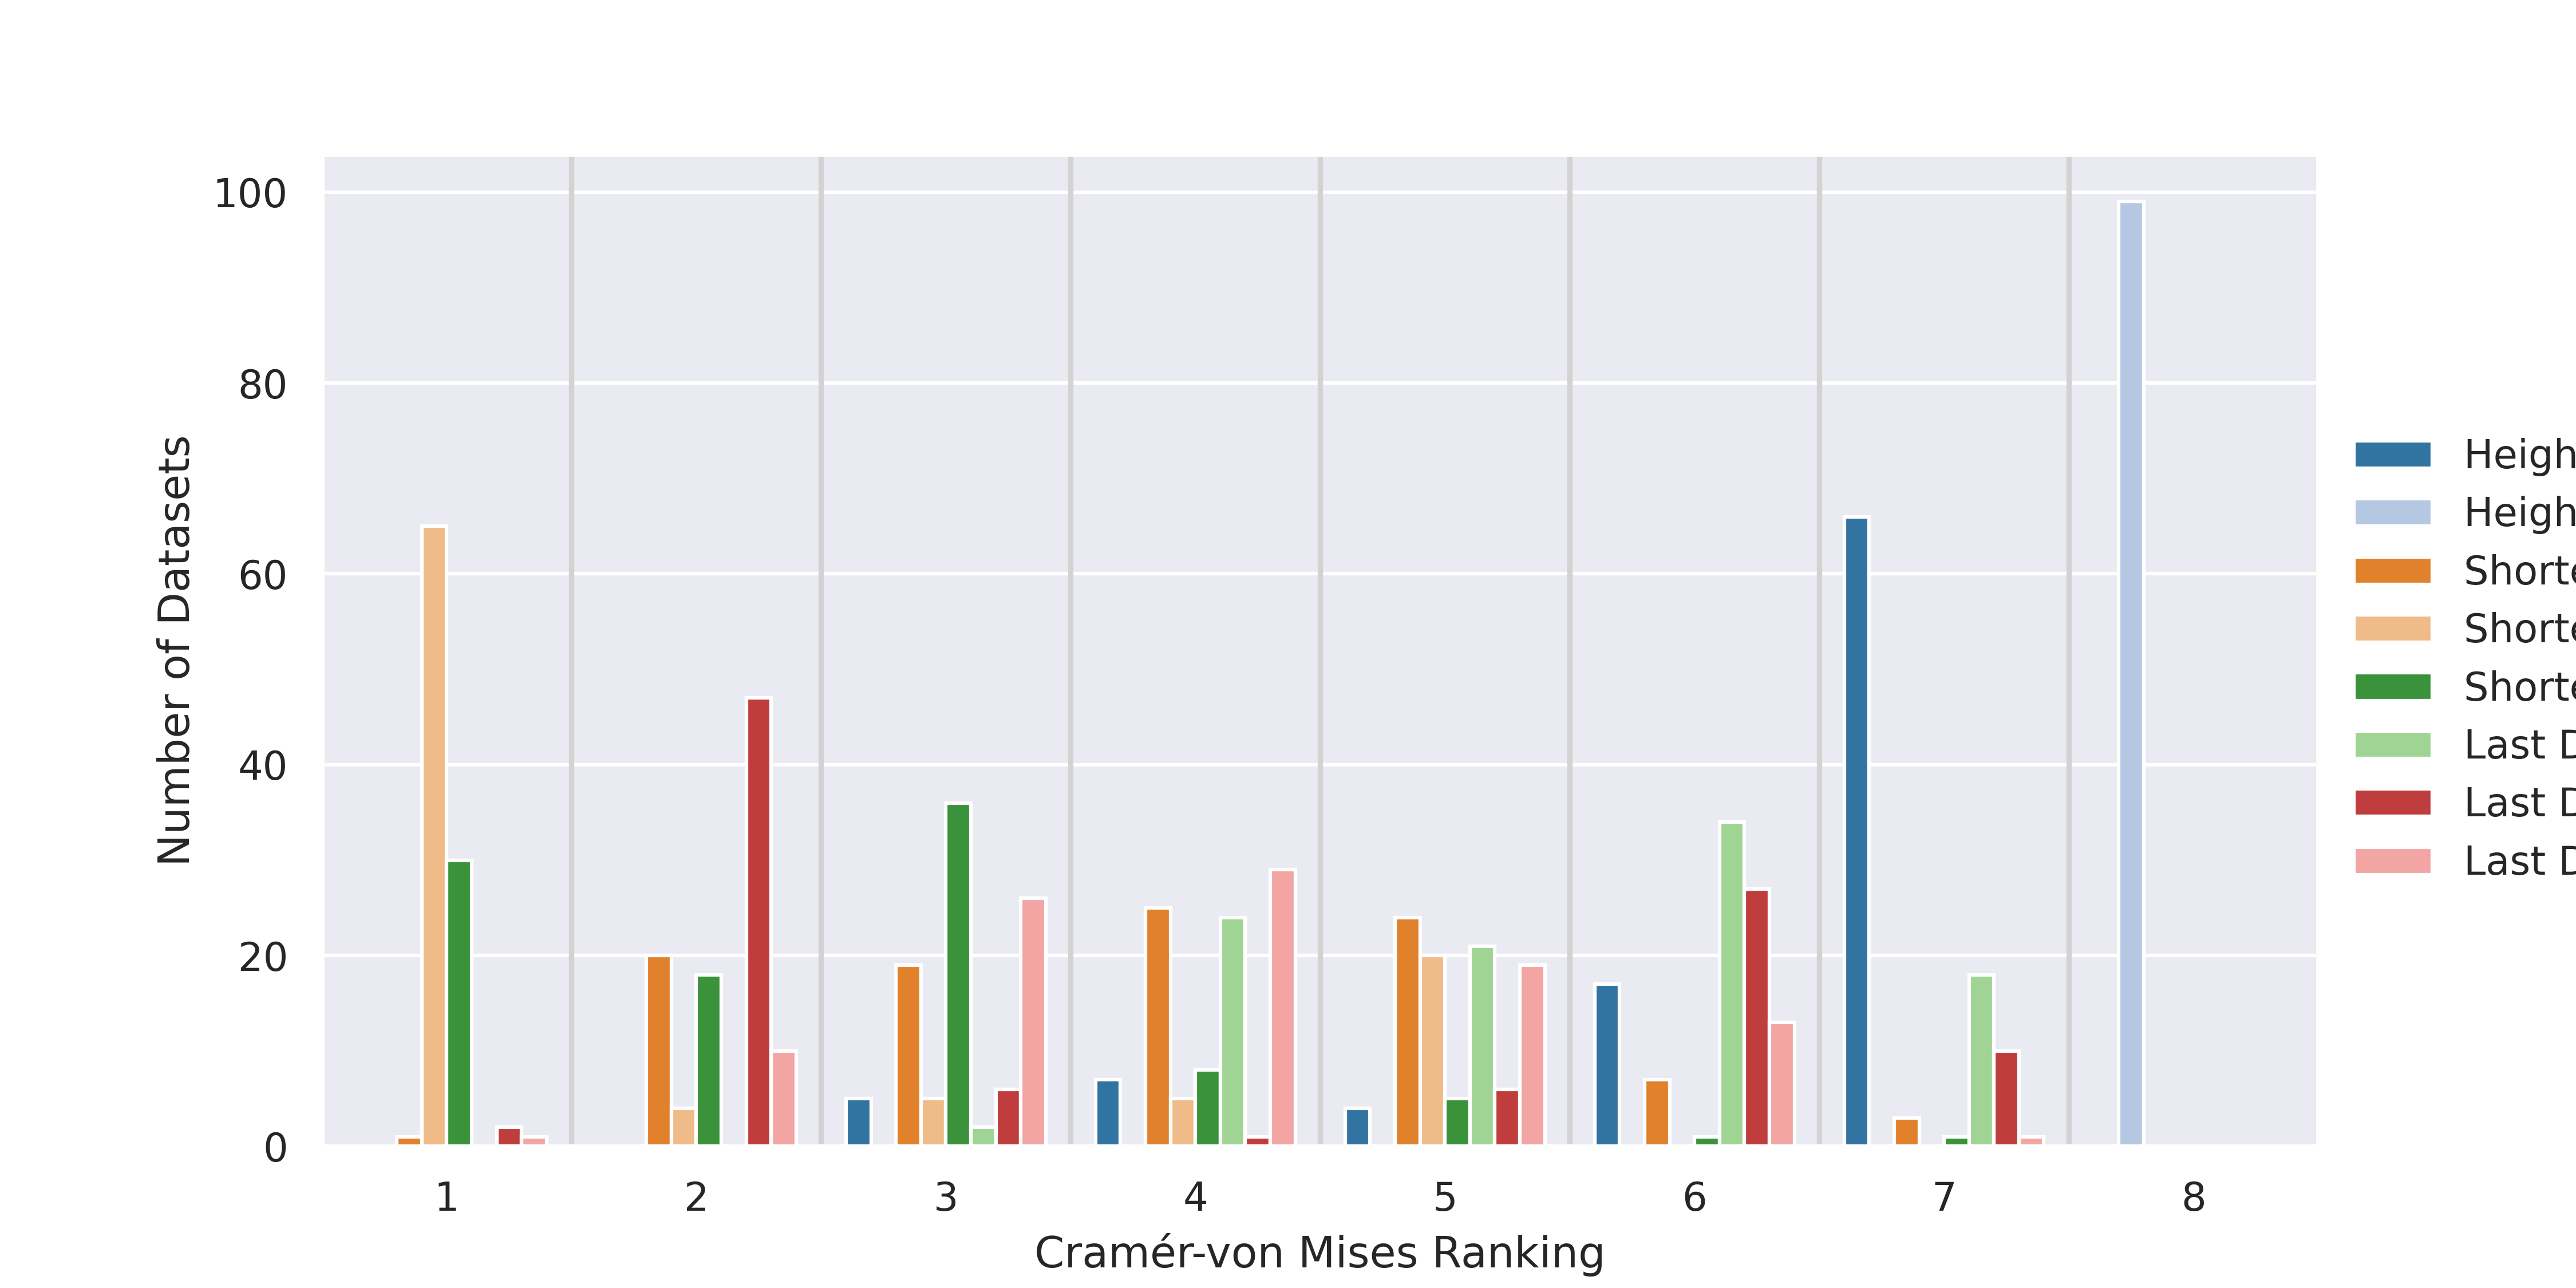
\includegraphics[width=\textwidth]{figures/yule-400-ccd1-cvm-ranking.png}
		\subcaption{Yule-400}
	\end{subfigure}
	\begin{subfigure}[b]{0.45\textwidth}
		\centering
		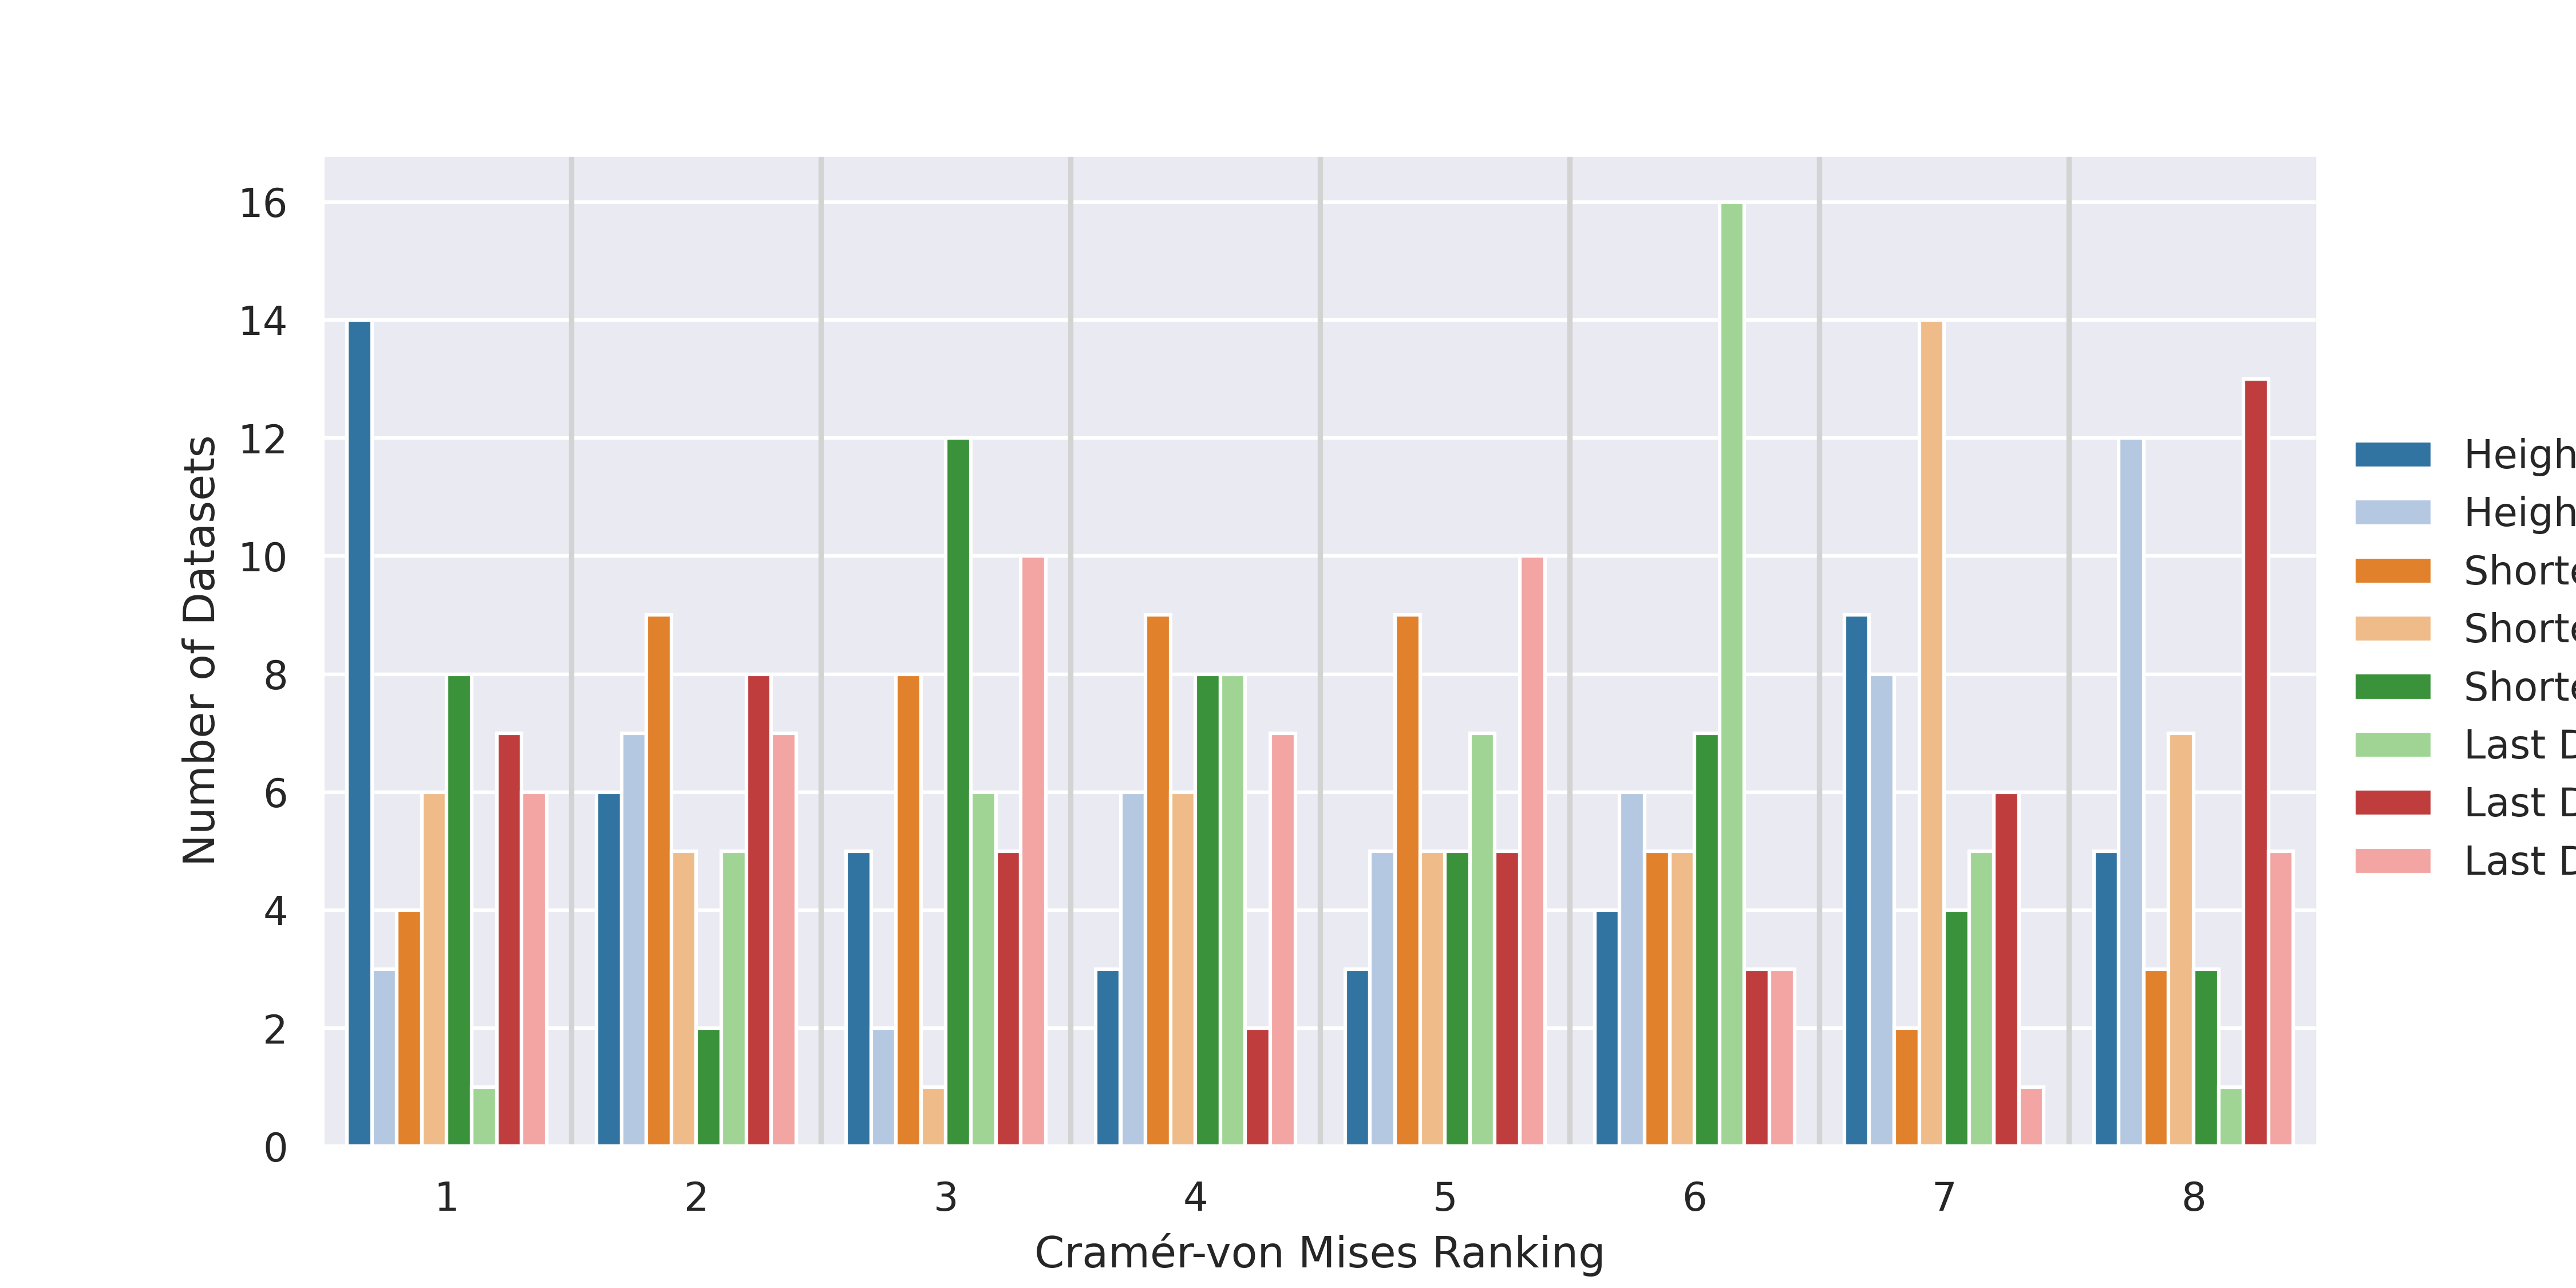
\includegraphics[width=\textwidth]{figures/bio-ccd1-cvm-ranking.png}
		\subcaption{Real-world datasets}
	\end{subfigure}
	
	\label{fig:cramer-von-mises-ranking}
\end{figure}

Figure \ref{fig:credible-regions} shows a selection of credible-region plots for some datasets and distributions. Plots for all datasets and distributions can be found in the Supporting Information. The larger divergence for some biological datasets can partly be attributed to their large entropy and small ESS. Whenever a clade split appears in the validation samples but not in the training samples, the corresponding CCD1 probability of a tree with this clade split collapses to $0$. These trees with probability $0$ are only contained in the smallest 100\%-credible region, leading to a smaller fraction than expected for all other credible regions. For 11 out of the 49 real-world datasets, every single tree in the validation sample has a probability of $0$.

\begin{figure}
	\caption{The credible-region plots for different datasets and distributions. The plot shows the fraction of MCMC trees contained in the smallest $\gamma$-credible region for different $\gamma$. The closer the resulting line is to the $x=y$ line the better. The blue line shows the median line for the datasets; 95 \% of all datasets fall into the blue region. The grey lines the credible-region plots for 10 random datasets.}
	
	\centering
	\begin{subfigure}[b]{0.45\textwidth}
		\centering
		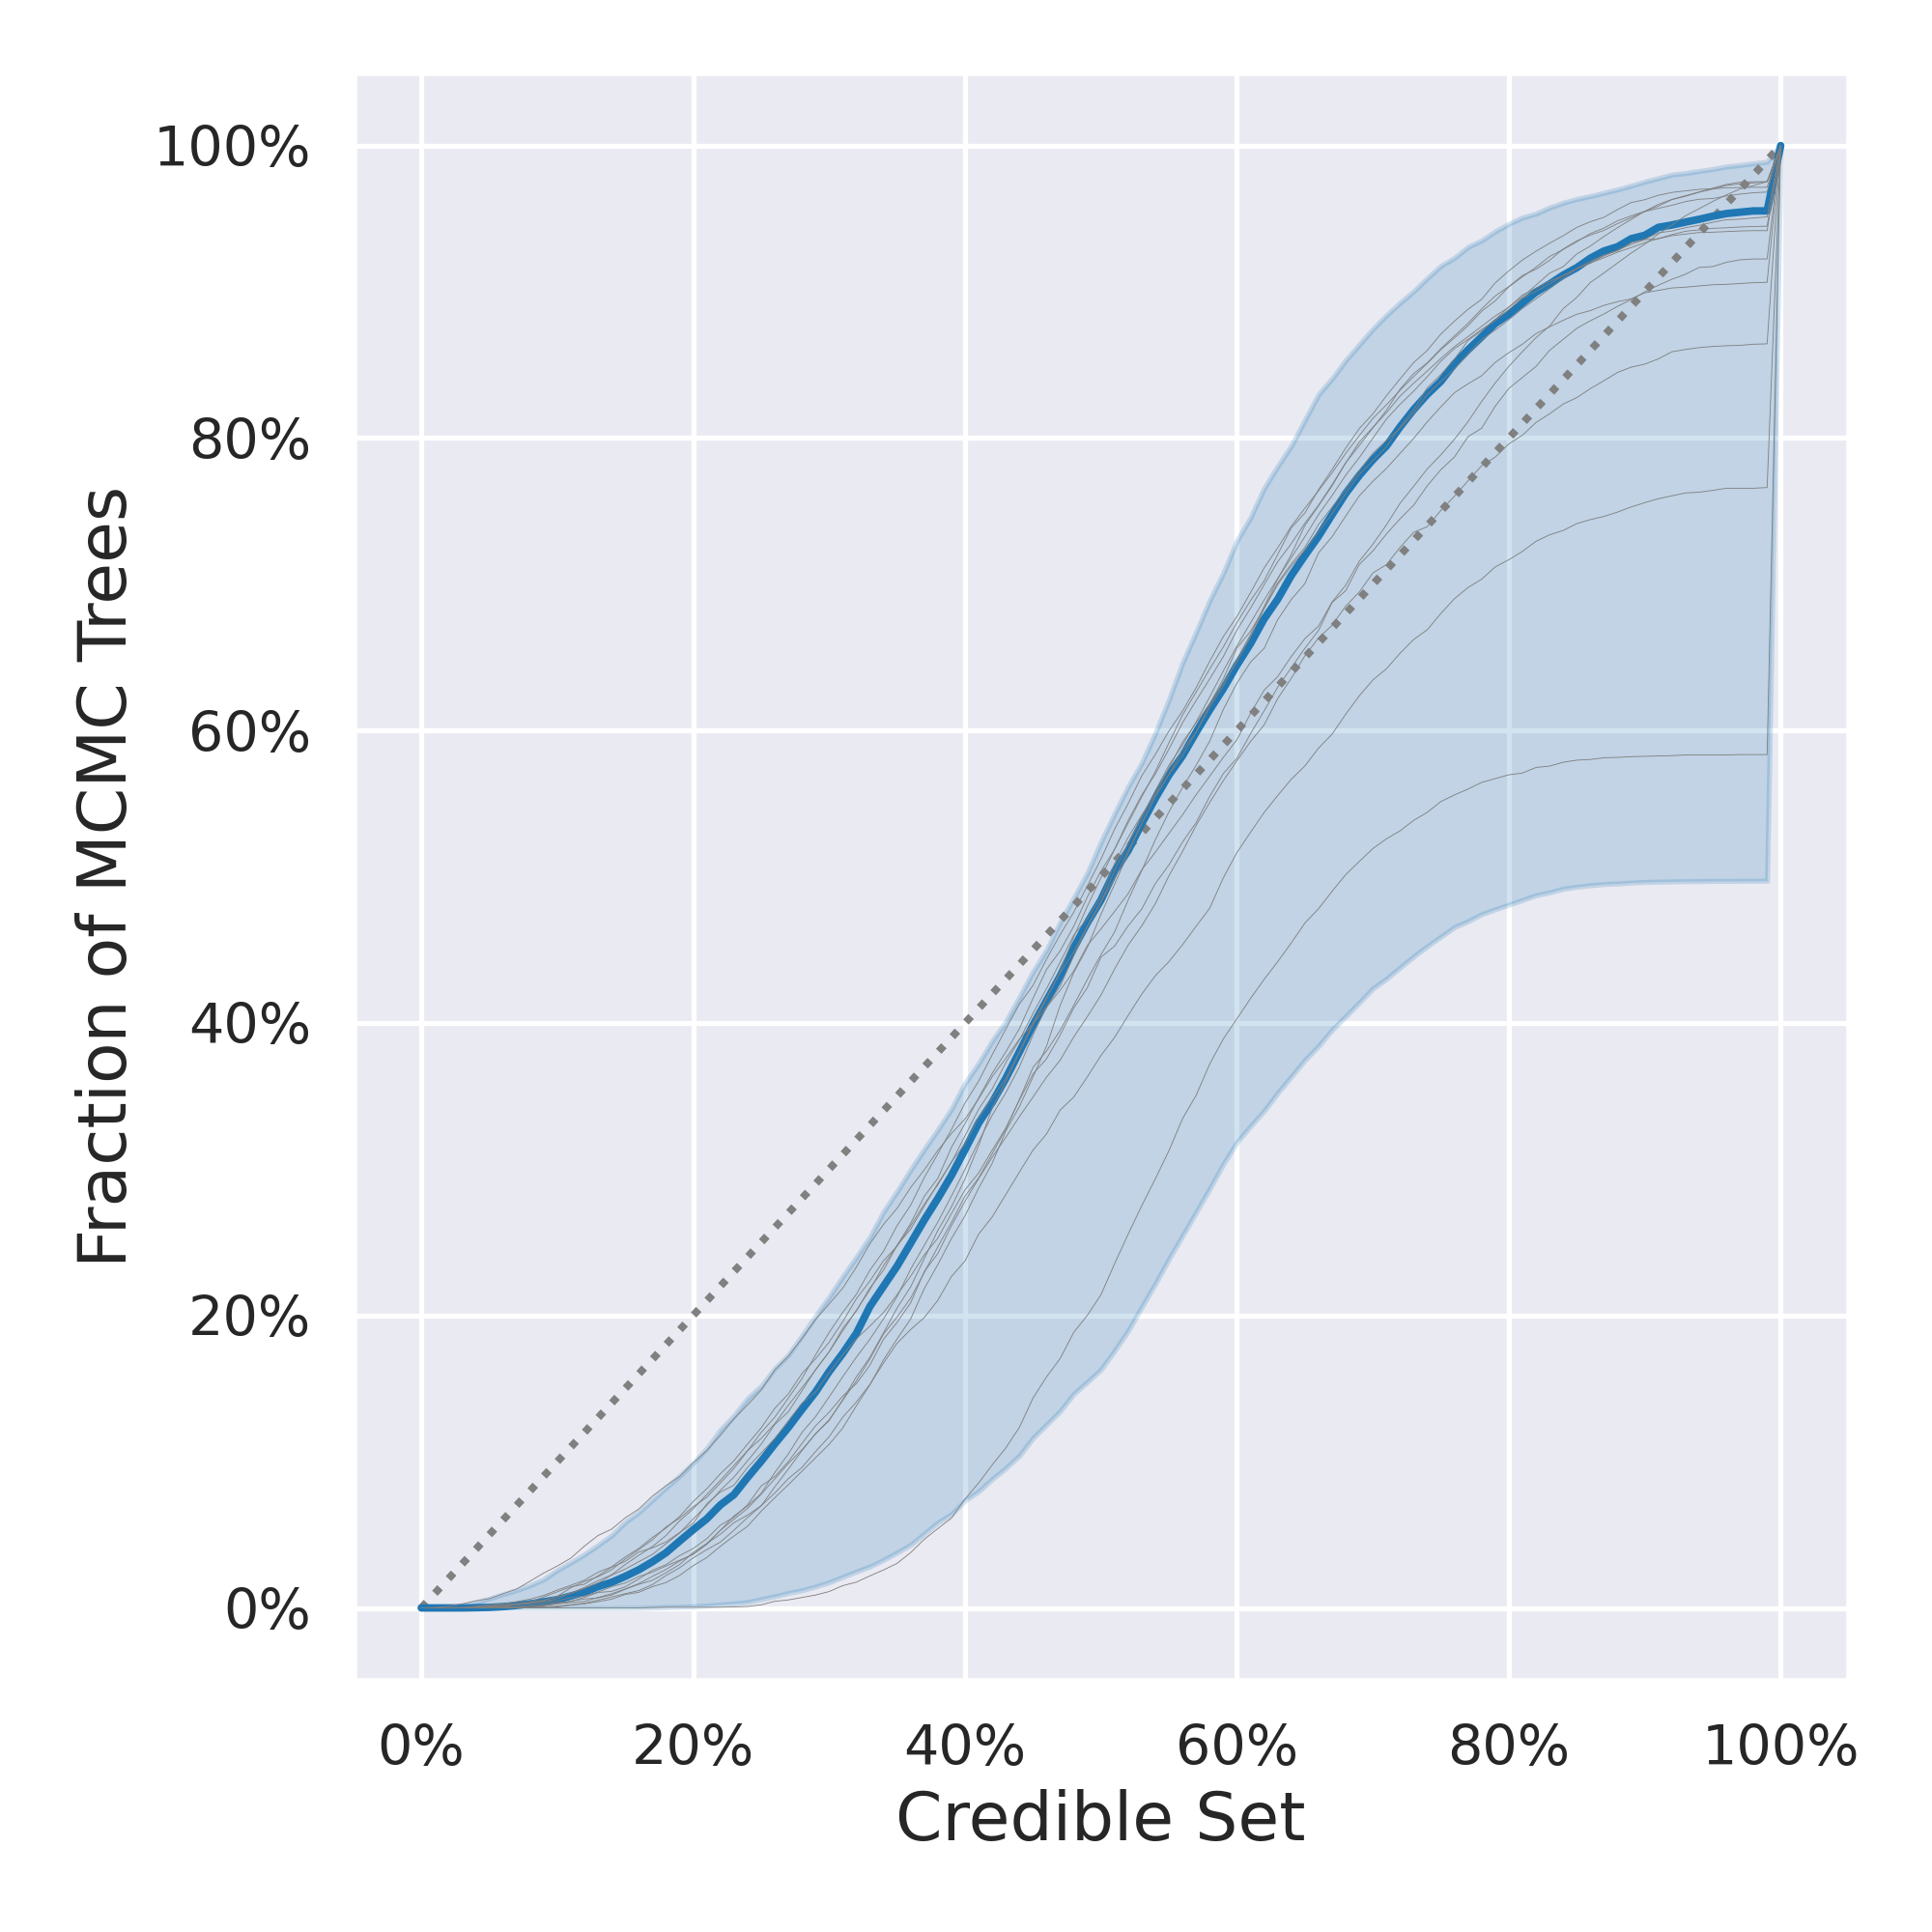
\includegraphics[width=\textwidth]{figures/yule-200-ccd1-credible-sets-Height (LogNormal), Ratios (Beta).png}
		\subcaption{Height (LogNormal), Ratios (Beta) on Yule-200}
	\end{subfigure}
	\begin{subfigure}[b]{0.4\textwidth}
		\centering
		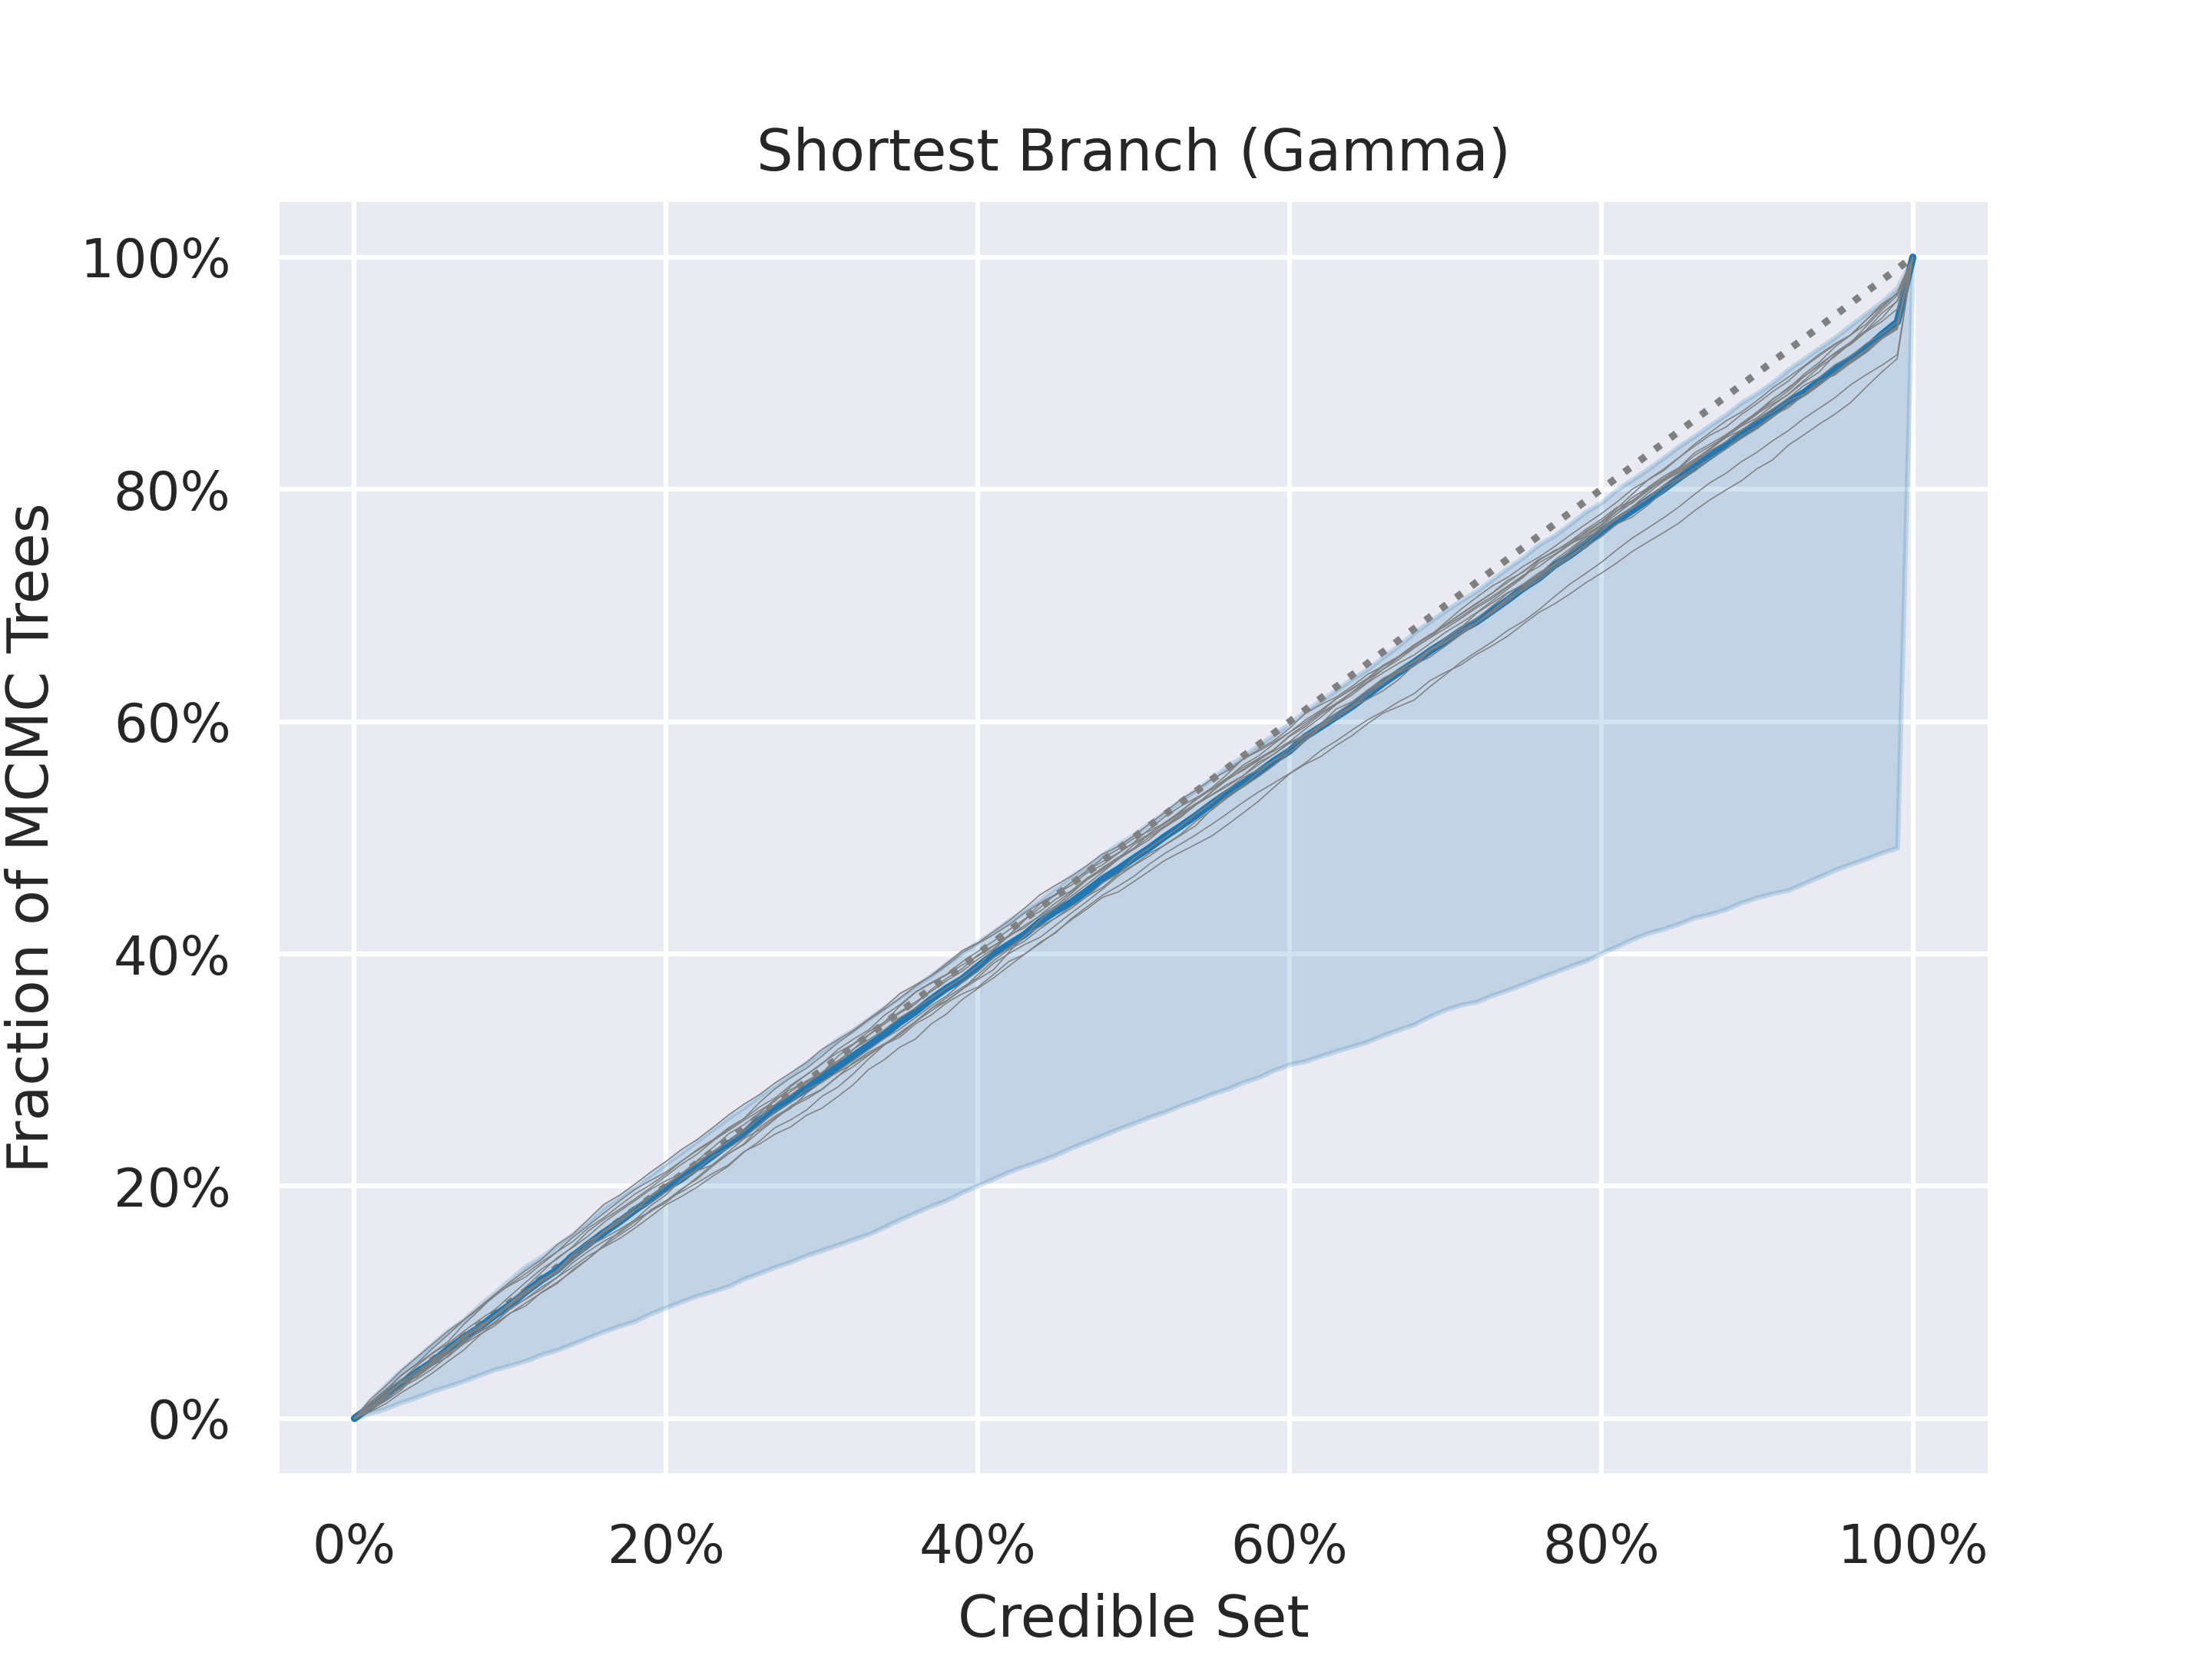
\includegraphics[width=\textwidth]{figures/yule-200-ccd1-credible-sets-Shortest Branch (Gamma).png}
		\subcaption{Shortest Branch (Gamma) on Yule-200}
	\end{subfigure}
	
	\begin{subfigure}[b]{0.4\textwidth}
		\centering
		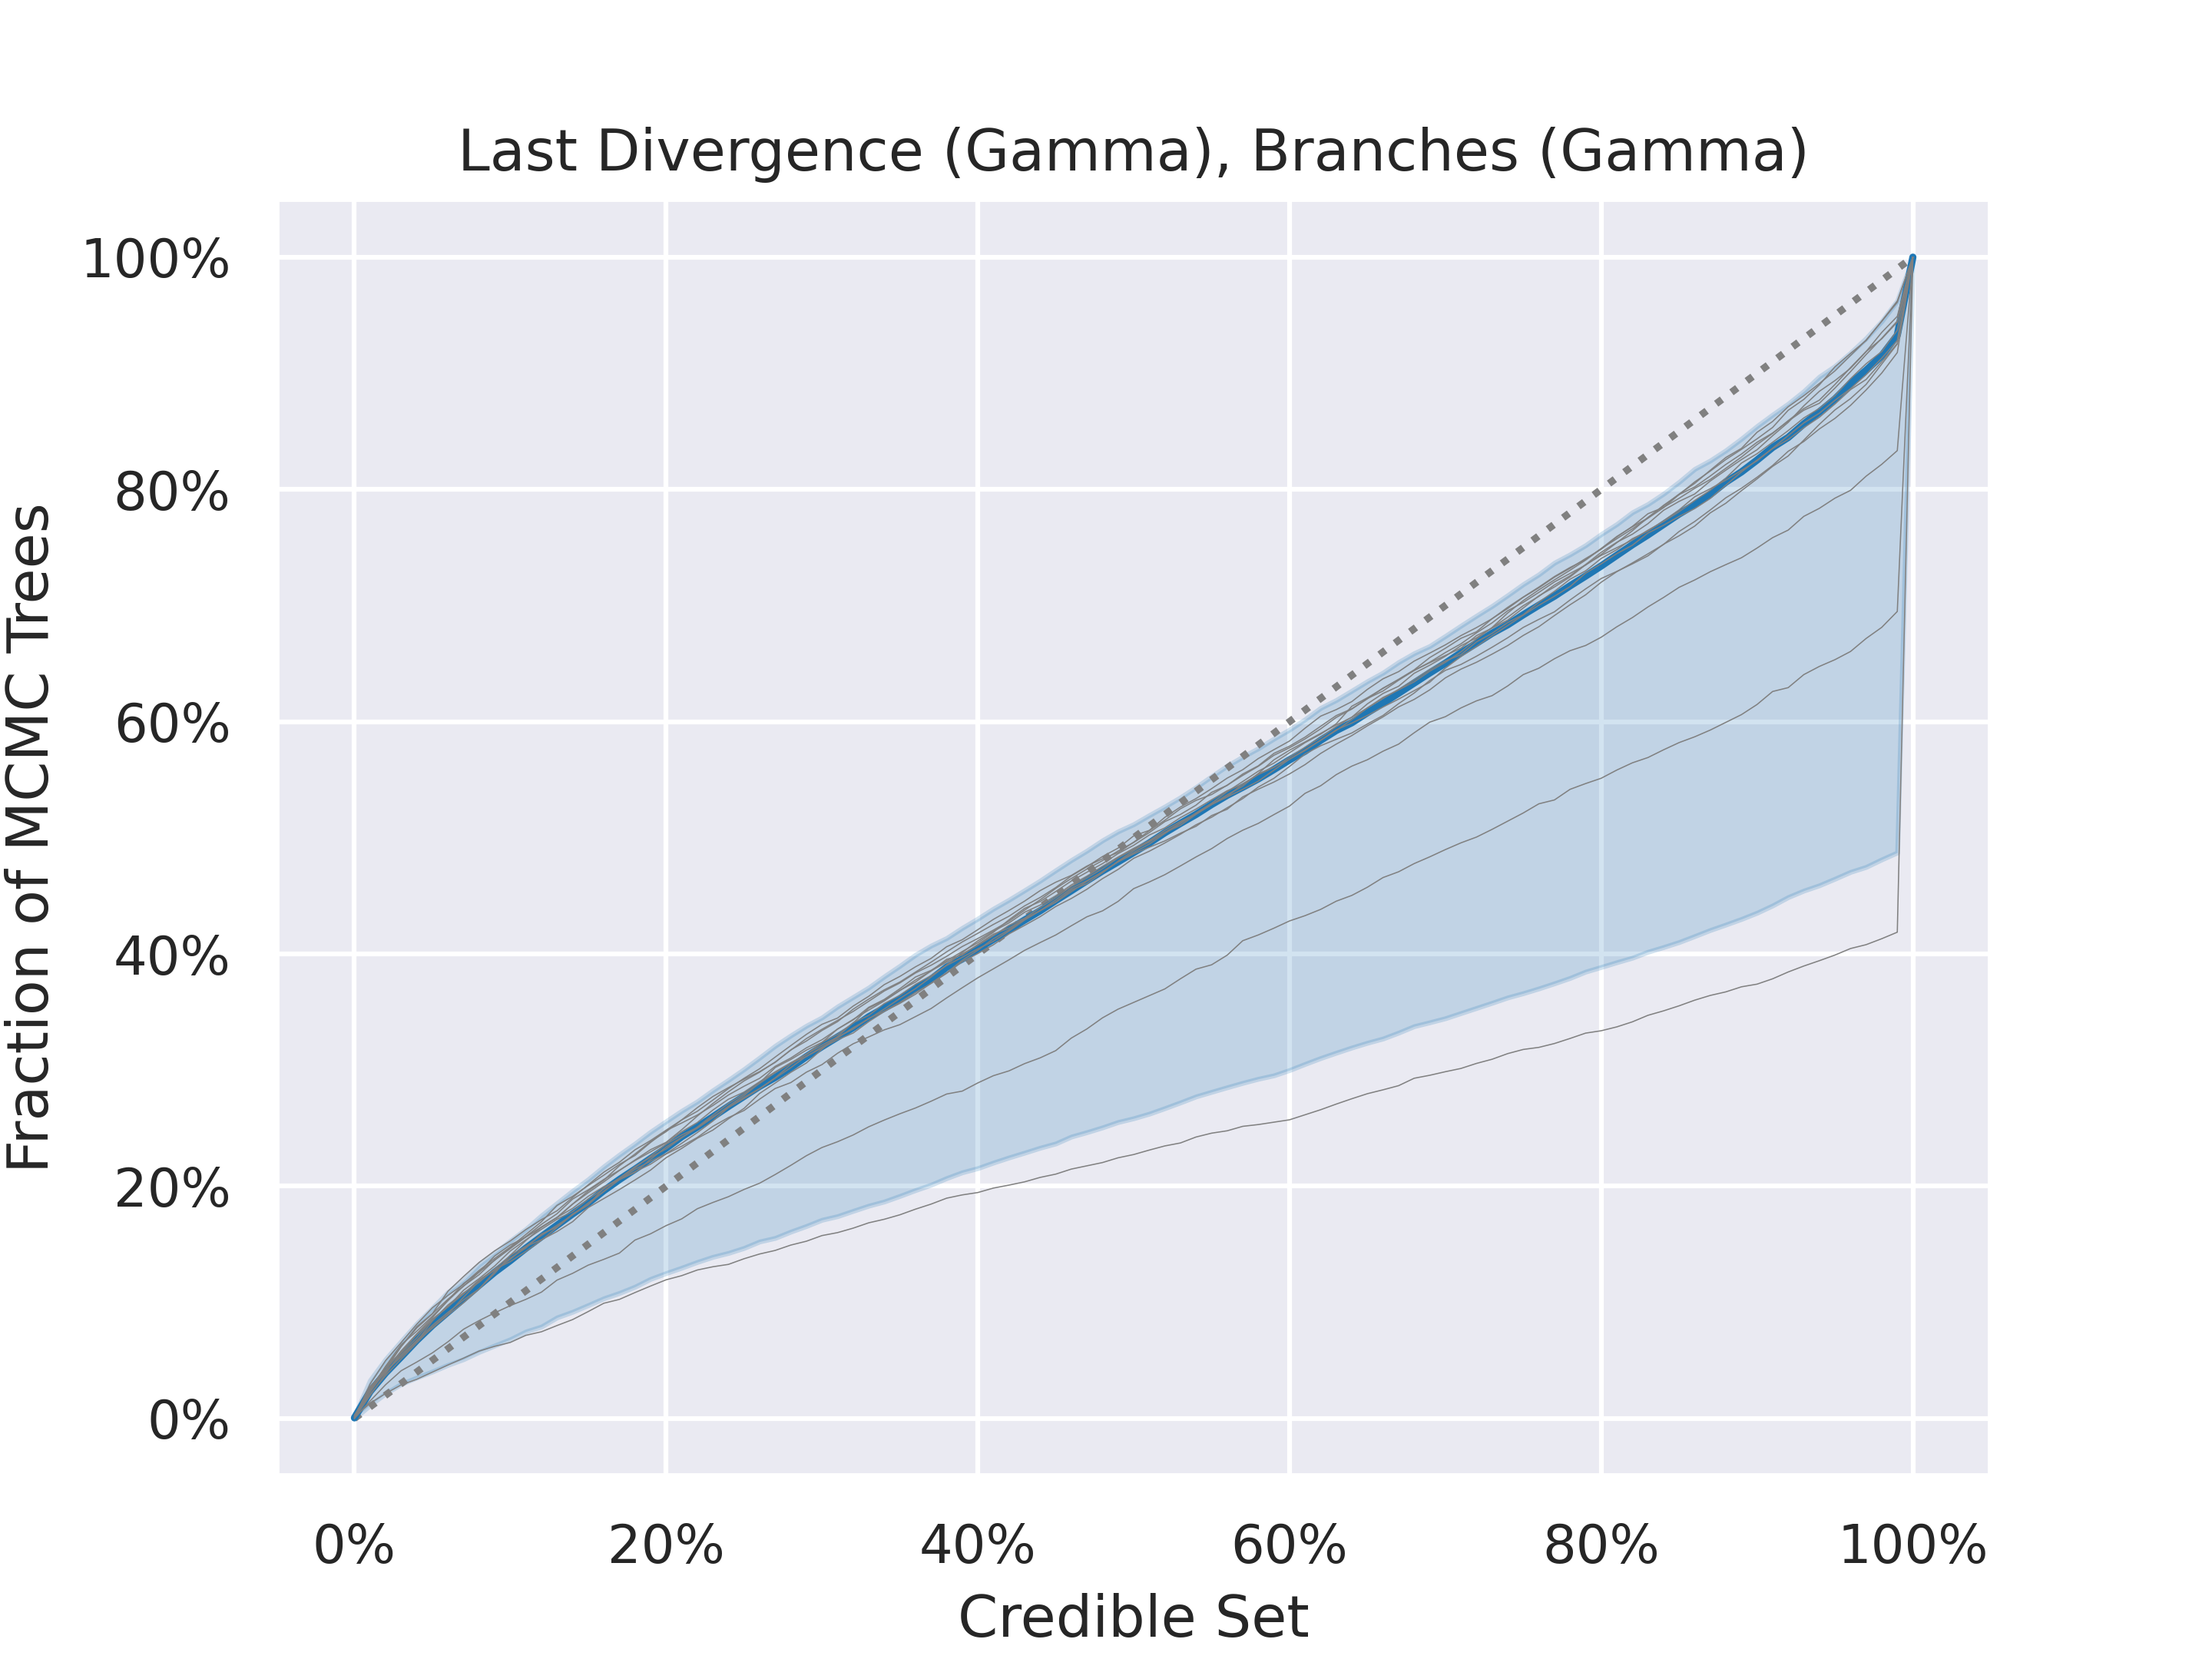
\includegraphics[width=\textwidth]{figures/yule-200-ccd1-credible-sets-Last Divergence (Gamma), Branches (Gamma).png}
		\subcaption{Last Divergence (Gamma), Branches (Gamma) on Yule-200}
	\end{subfigure}
	\begin{subfigure}[b]{0.4\textwidth}
		\centering
		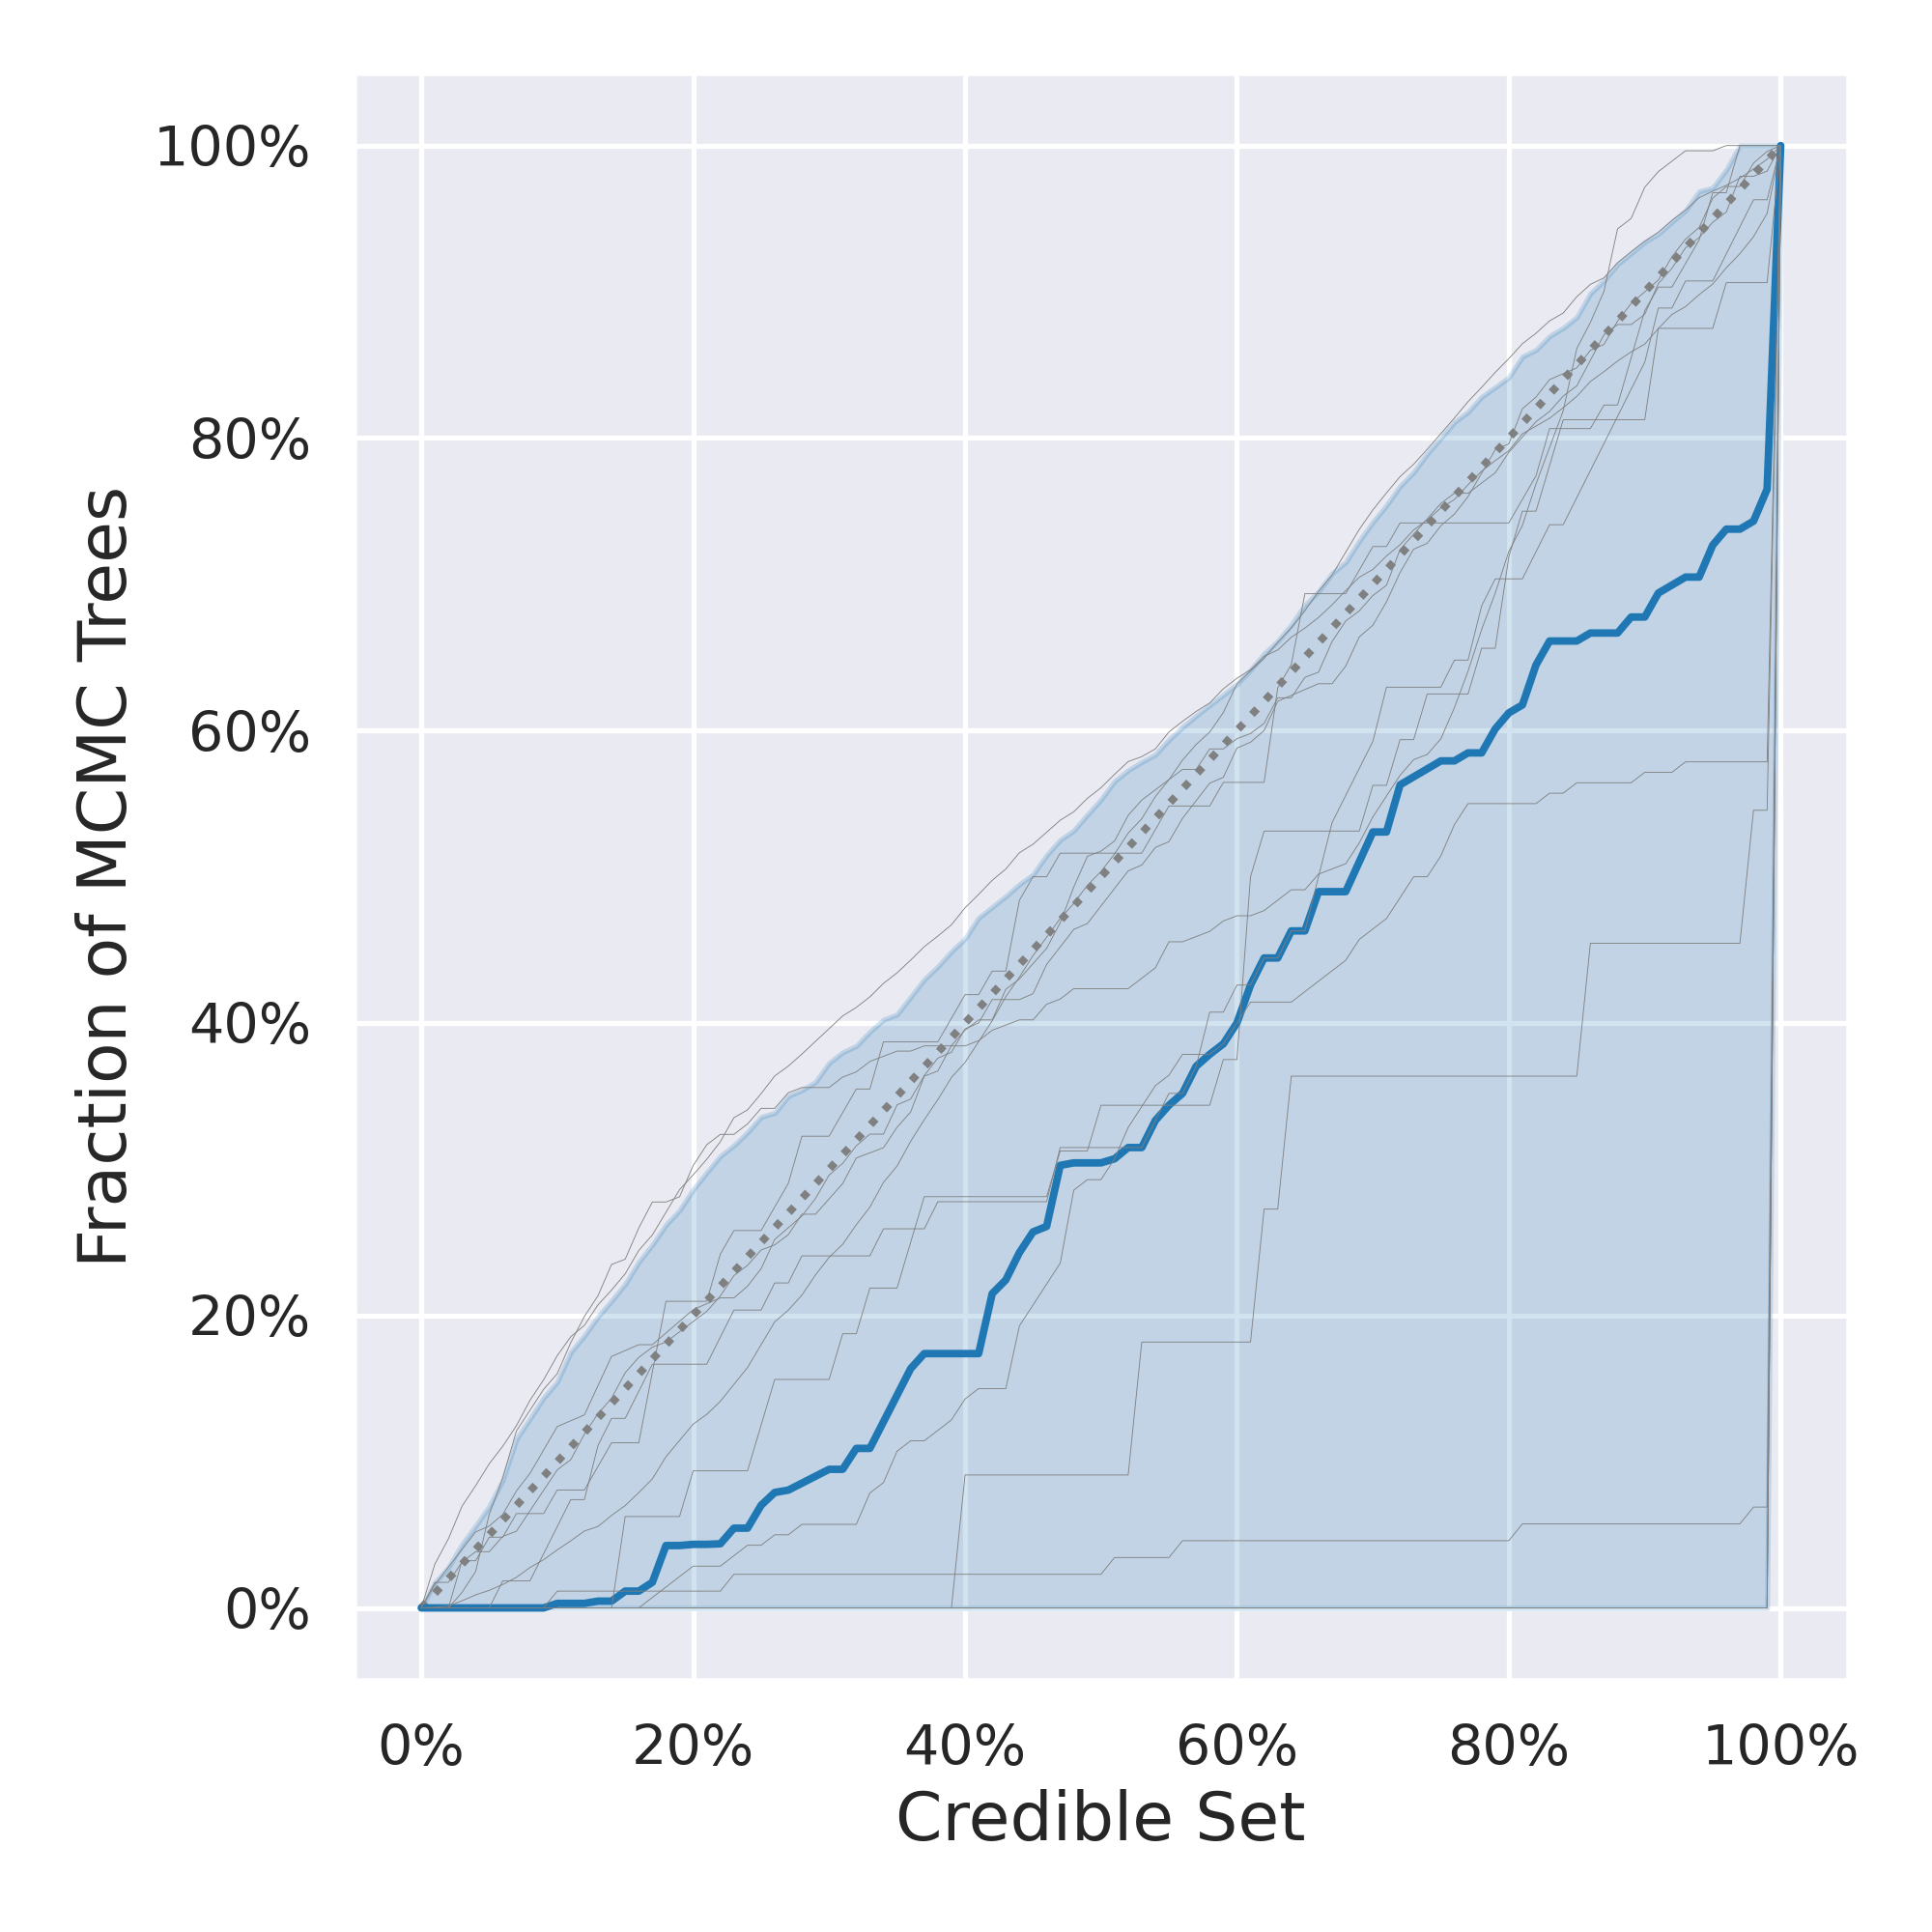
\includegraphics[width=\textwidth]{figures/bio-ccd1-credible-sets-Height (LogNormal), Ratios (Beta).png}
		\subcaption{Height (LogNormal), Ratios (Beta) on real-world datasets}
	\end{subfigure}

	\begin{subfigure}[b]{0.4\textwidth}
		\centering
		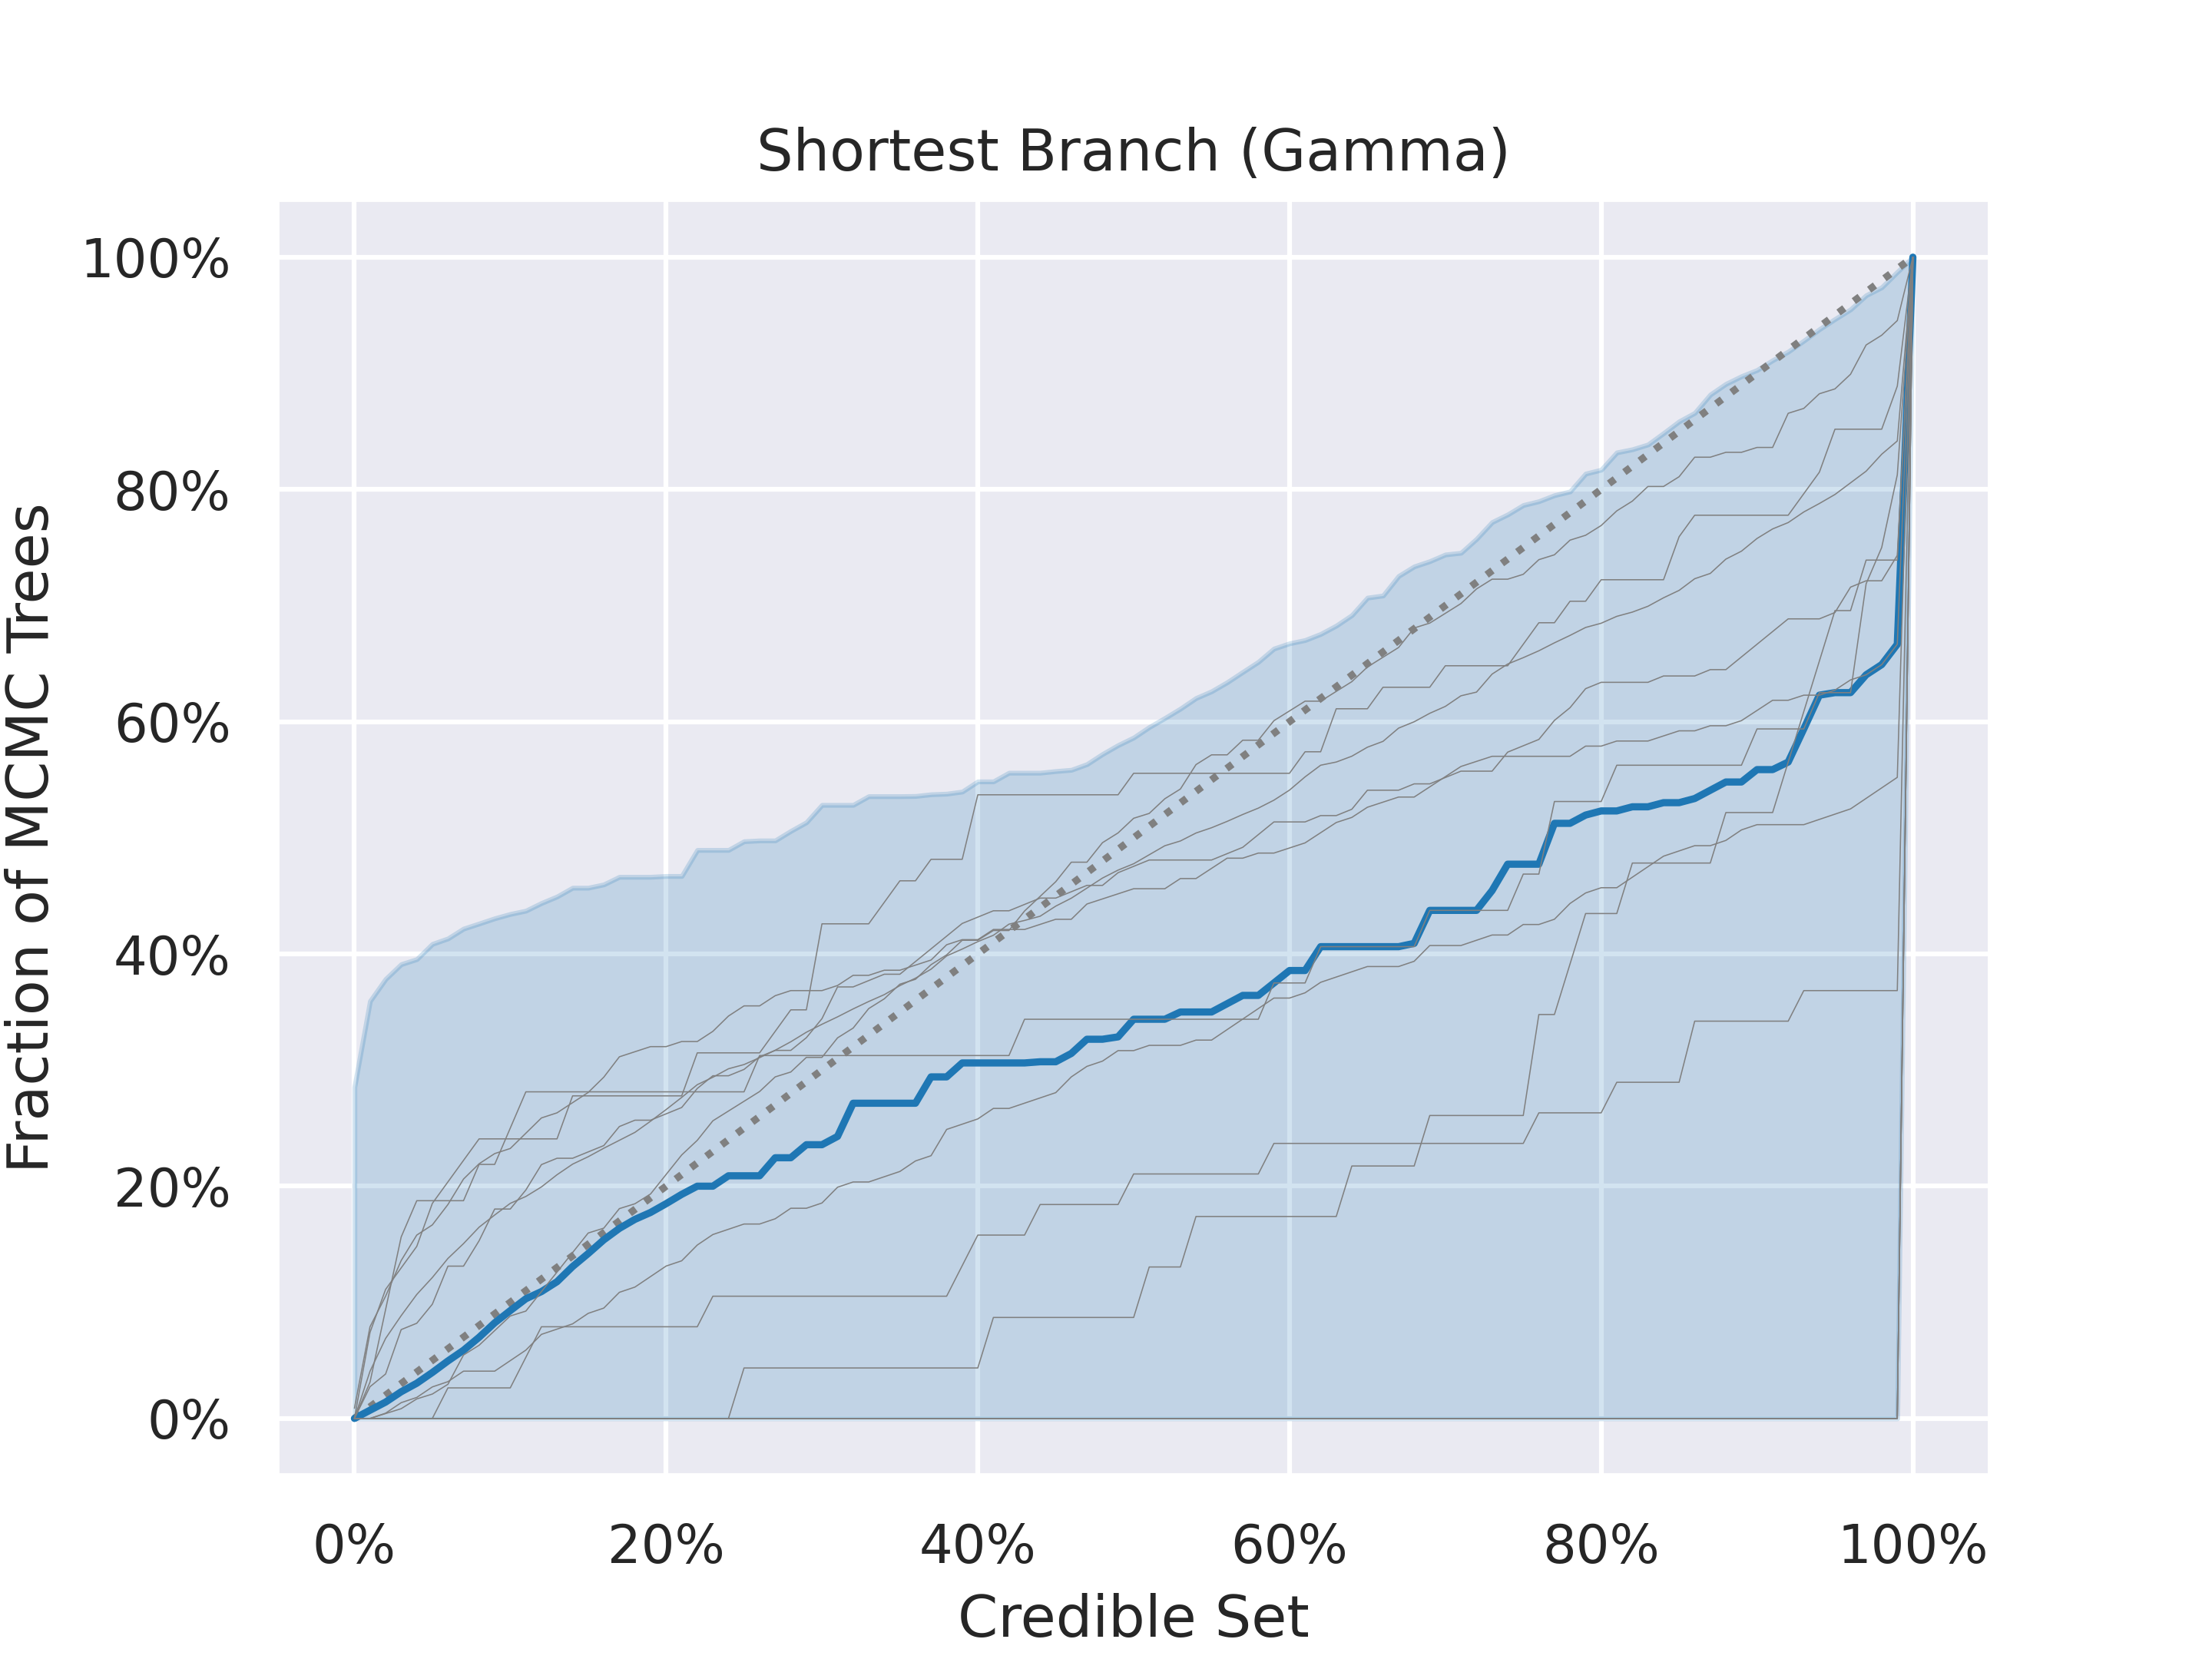
\includegraphics[width=\textwidth]{figures/bio-ccd1-credible-sets-Shortest Branch (Gamma).png}
		\subcaption{Shortest Branch (Gamma) on real-world datasets}
	\end{subfigure}
	\begin{subfigure}[b]{0.4\textwidth}
		\centering
		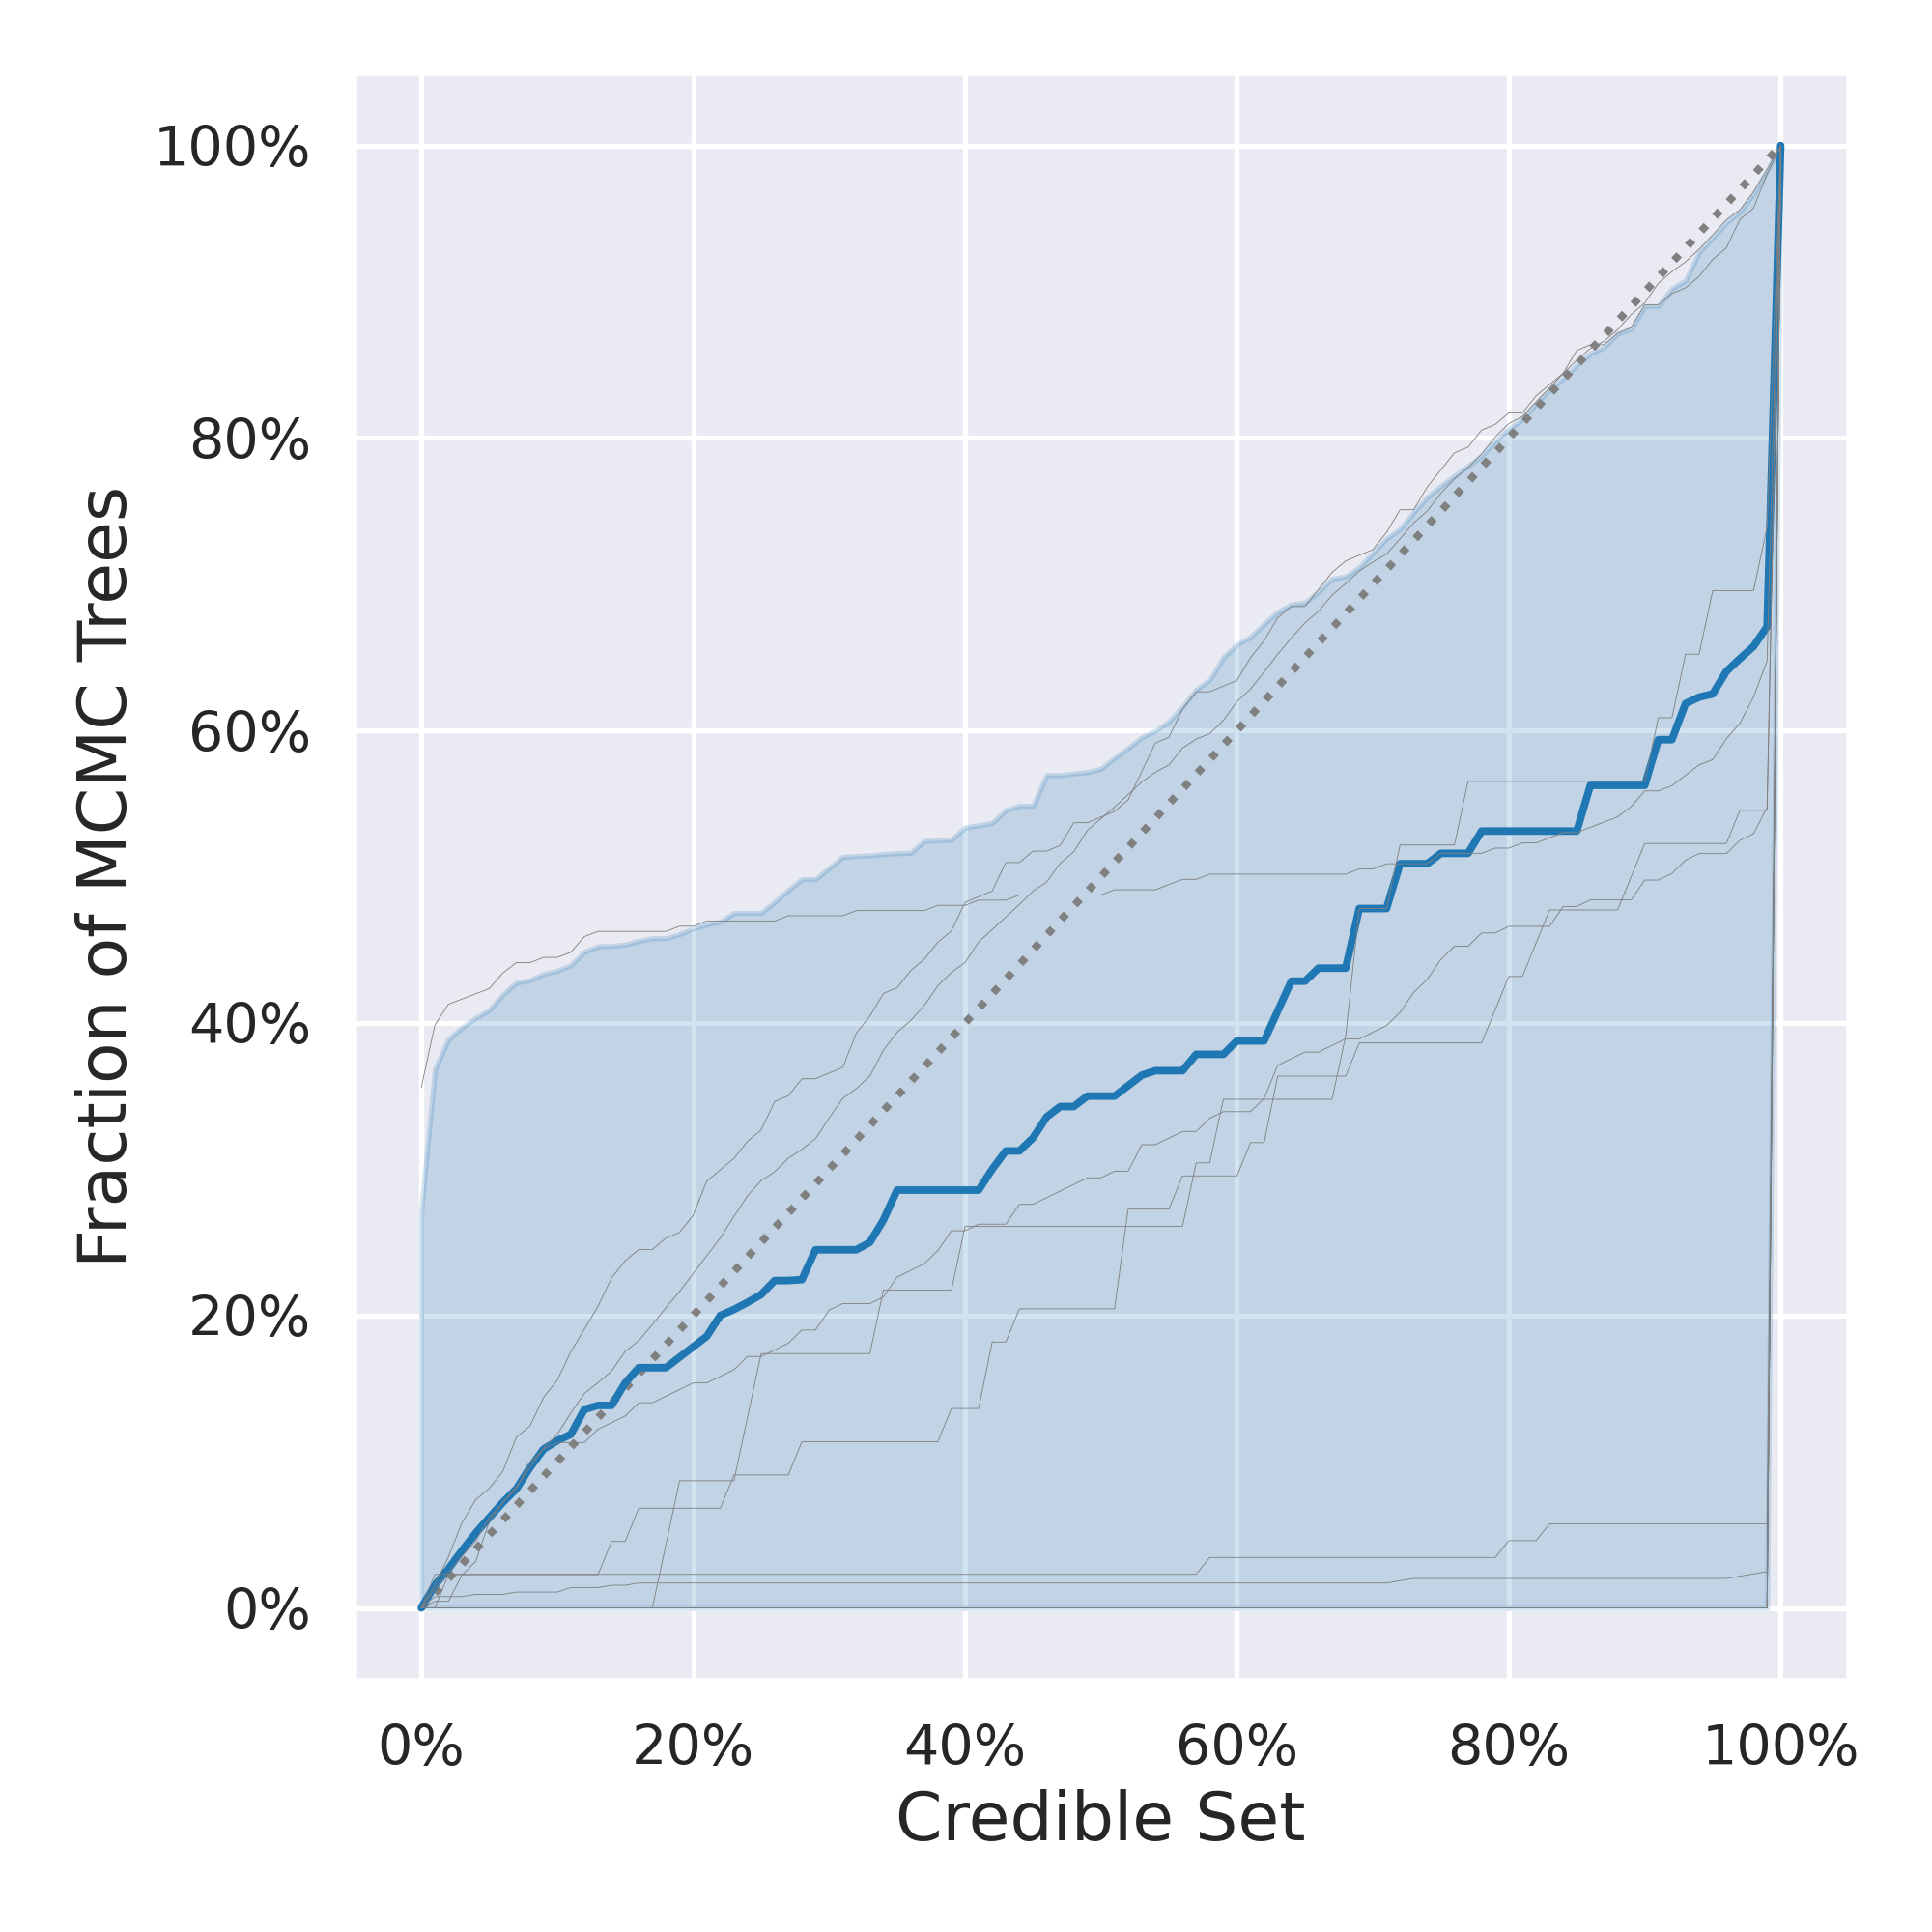
\includegraphics[width=\textwidth]{figures/bio-ccd1-credible-sets-Last Divergence (Gamma), Branches (Gamma).png}
		\subcaption{Last Divergence (Gamma), Branches (Gamma) on real-world datasets}
	\end{subfigure}
	
	\label{fig:credible-regions}
\end{figure}

\subsection*{Accuracy of the point estimators}

With the simulated datasets, we have access to the true tree, allowing us to assess point estimator accuracy. We use the same topological point estimate (CCD1 MAP) for all models, focusing our comparison on the vertex height estimates. The entire downsampled MCMC sample is used to fit the distributions for the point estimates, as we don't need a validation set for validation in this case. Figure \ref{fig:accuracy-point-estimators} displays the distance to the true tree for the different distributions (and MRCA) and simulated datasets. Figure \ref{fig:accuracy-point-estimators-ranking} shows how often a specific method ranks at a certain position when compared to the other methods. It is apparant that none of the presented methods performs better than MRCA for a majority of datasets. However, ignoring the last divergence embeddings, all methods produce point estimates of similar quality.

\begin{figure}
	\caption{The log squared branch distance to the true tree for point estimates using the different distributions and datasets. (The lower the better.)}
	
	\centering
	\begin{subfigure}[b]{0.45\textwidth}
		\centering
		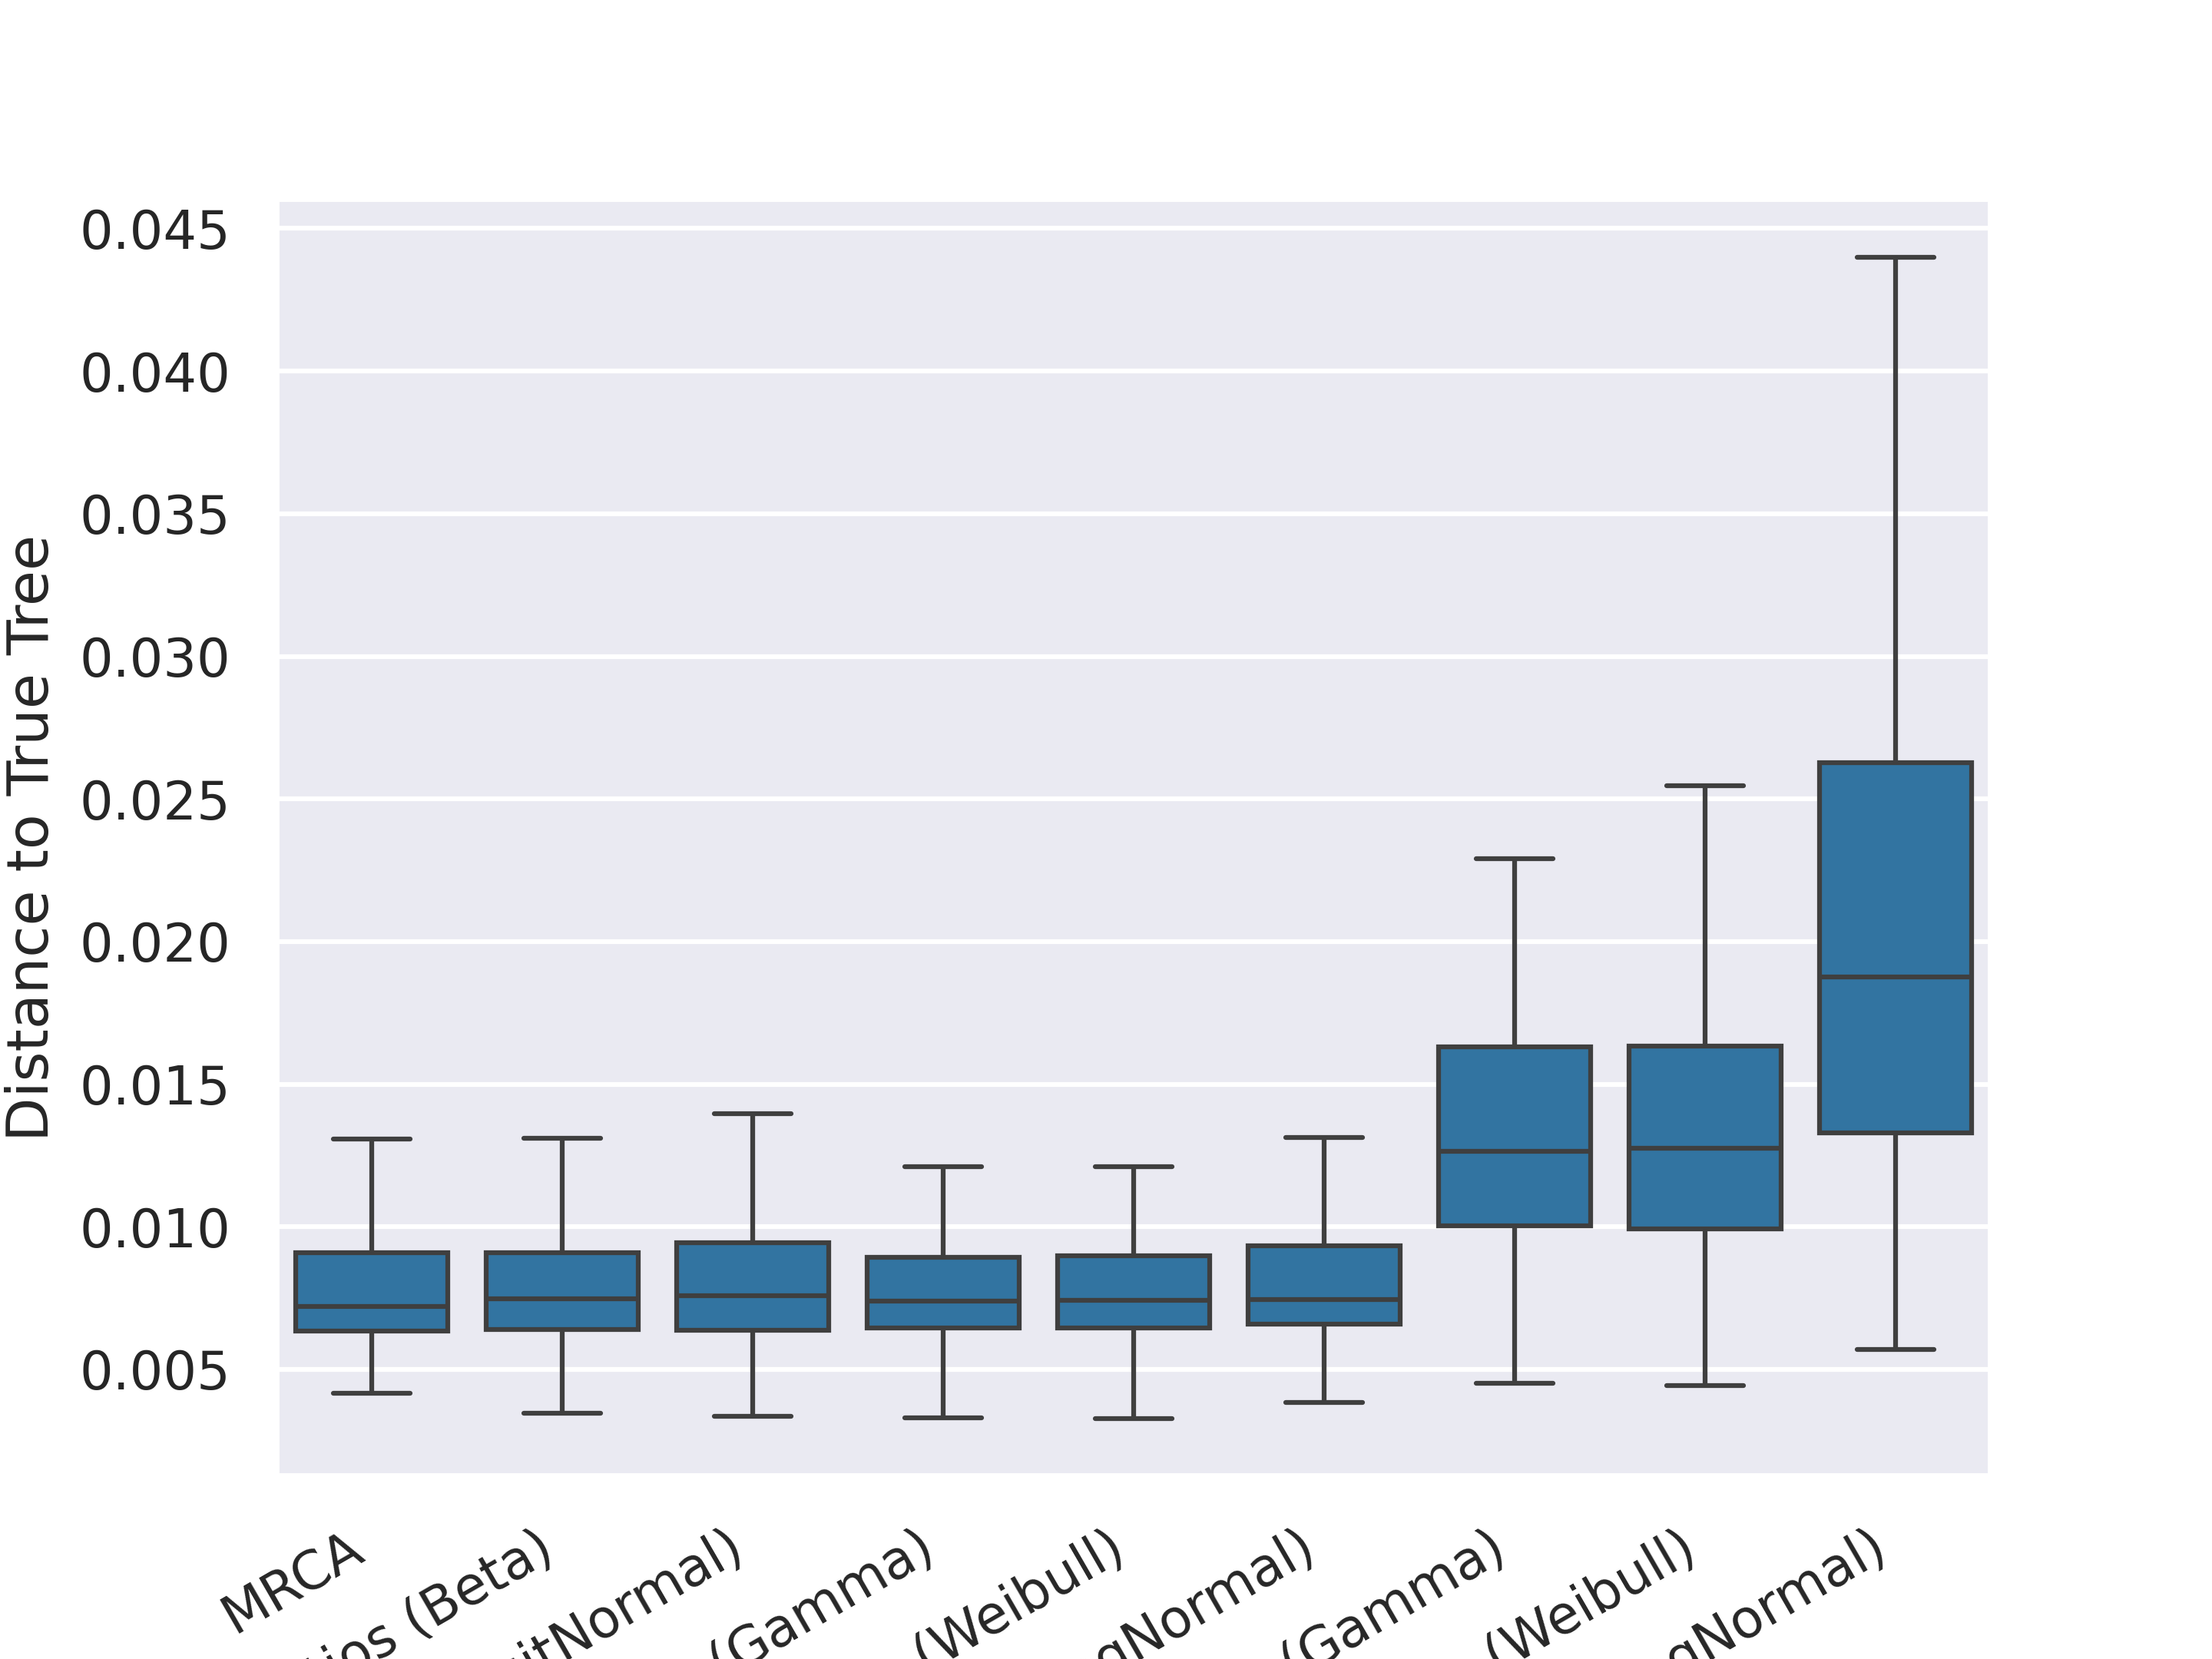
\includegraphics[width=\textwidth]{figures/yule-100-ccd1-point-estimates.png}
		\subcaption{Yule-100}
	\end{subfigure}
	\begin{subfigure}[b]{0.45\textwidth}
		\centering
		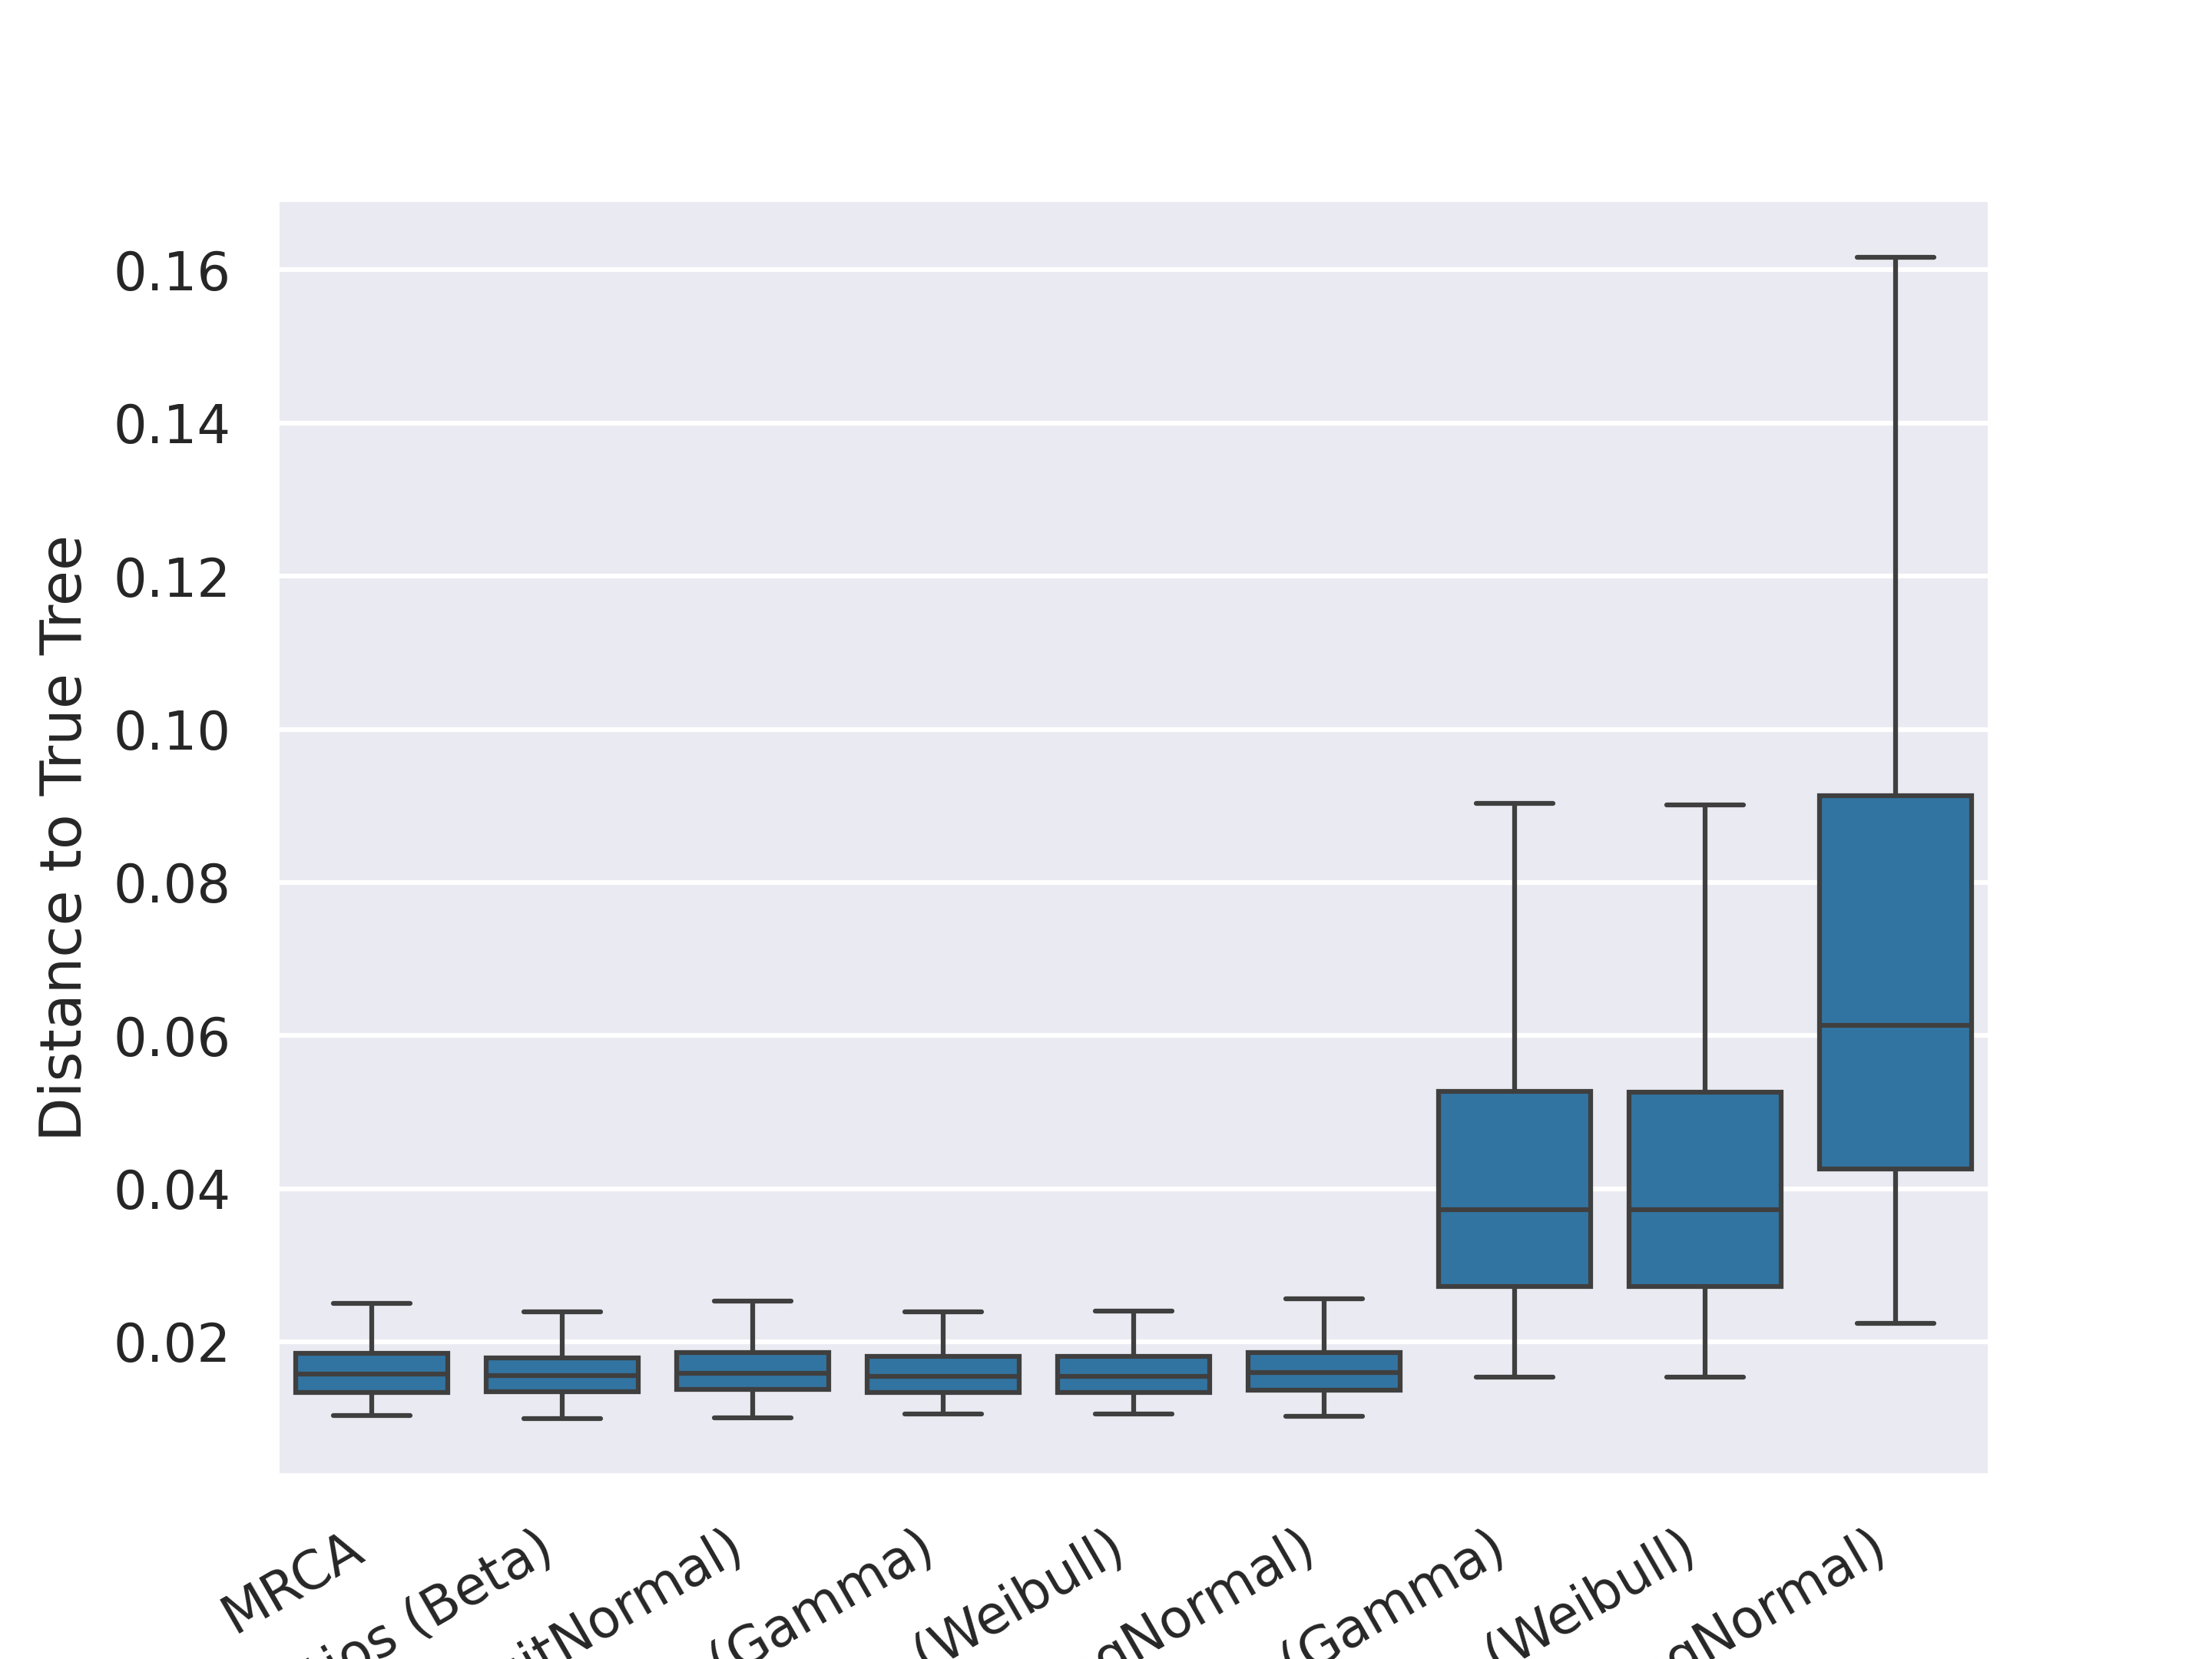
\includegraphics[width=\textwidth]{figures/yule-200-ccd1-point-estimates.png}
		\subcaption{Yule-200}
	\end{subfigure}
	
	\begin{subfigure}[b]{0.45\textwidth}
		\centering
		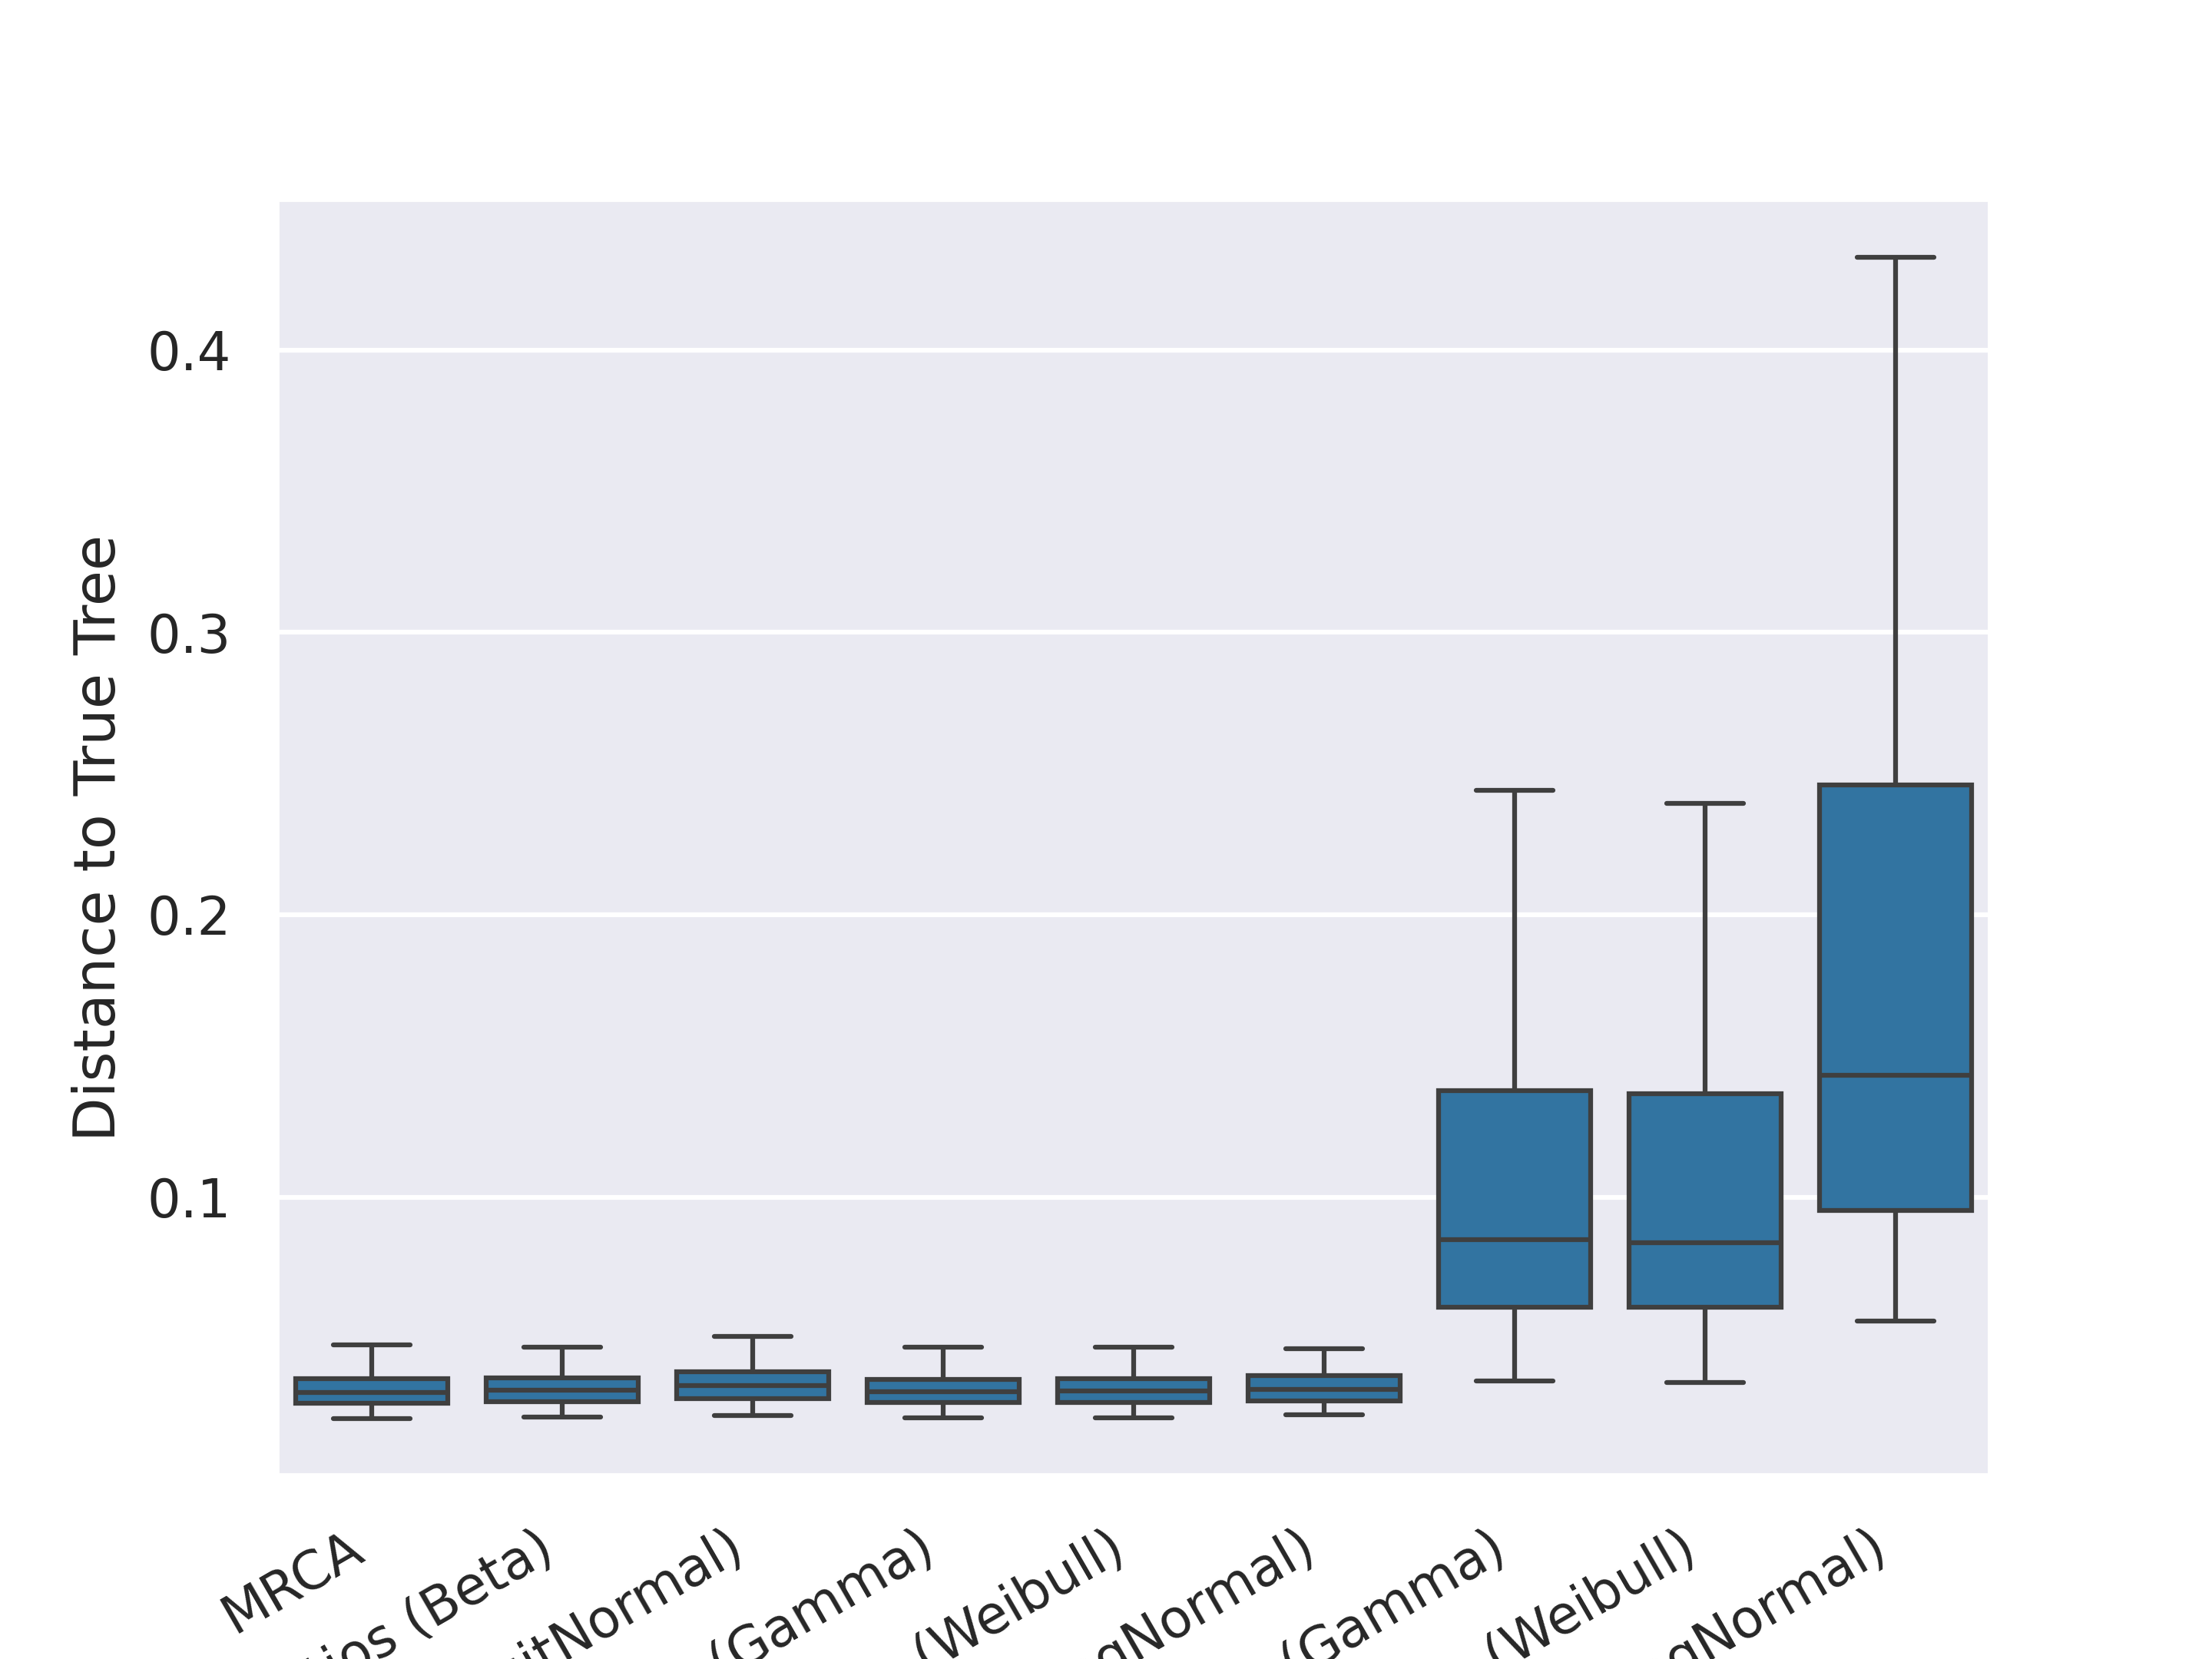
\includegraphics[width=\textwidth]{figures/yule-400-ccd1-point-estimates.png}
		\subcaption{Yule-400}
	\end{subfigure}
	
	\label{fig:accuracy-point-estimators}
\end{figure}

\begin{figure}
	\caption{How often each method ranked at a certain position when its point estimate is compared to the other methods. For example, MRCA ranked first for the majority of datasets. (The lower the rank the better.)}
	
	\centering
	\begin{subfigure}[b]{0.45\textwidth}
		\centering
		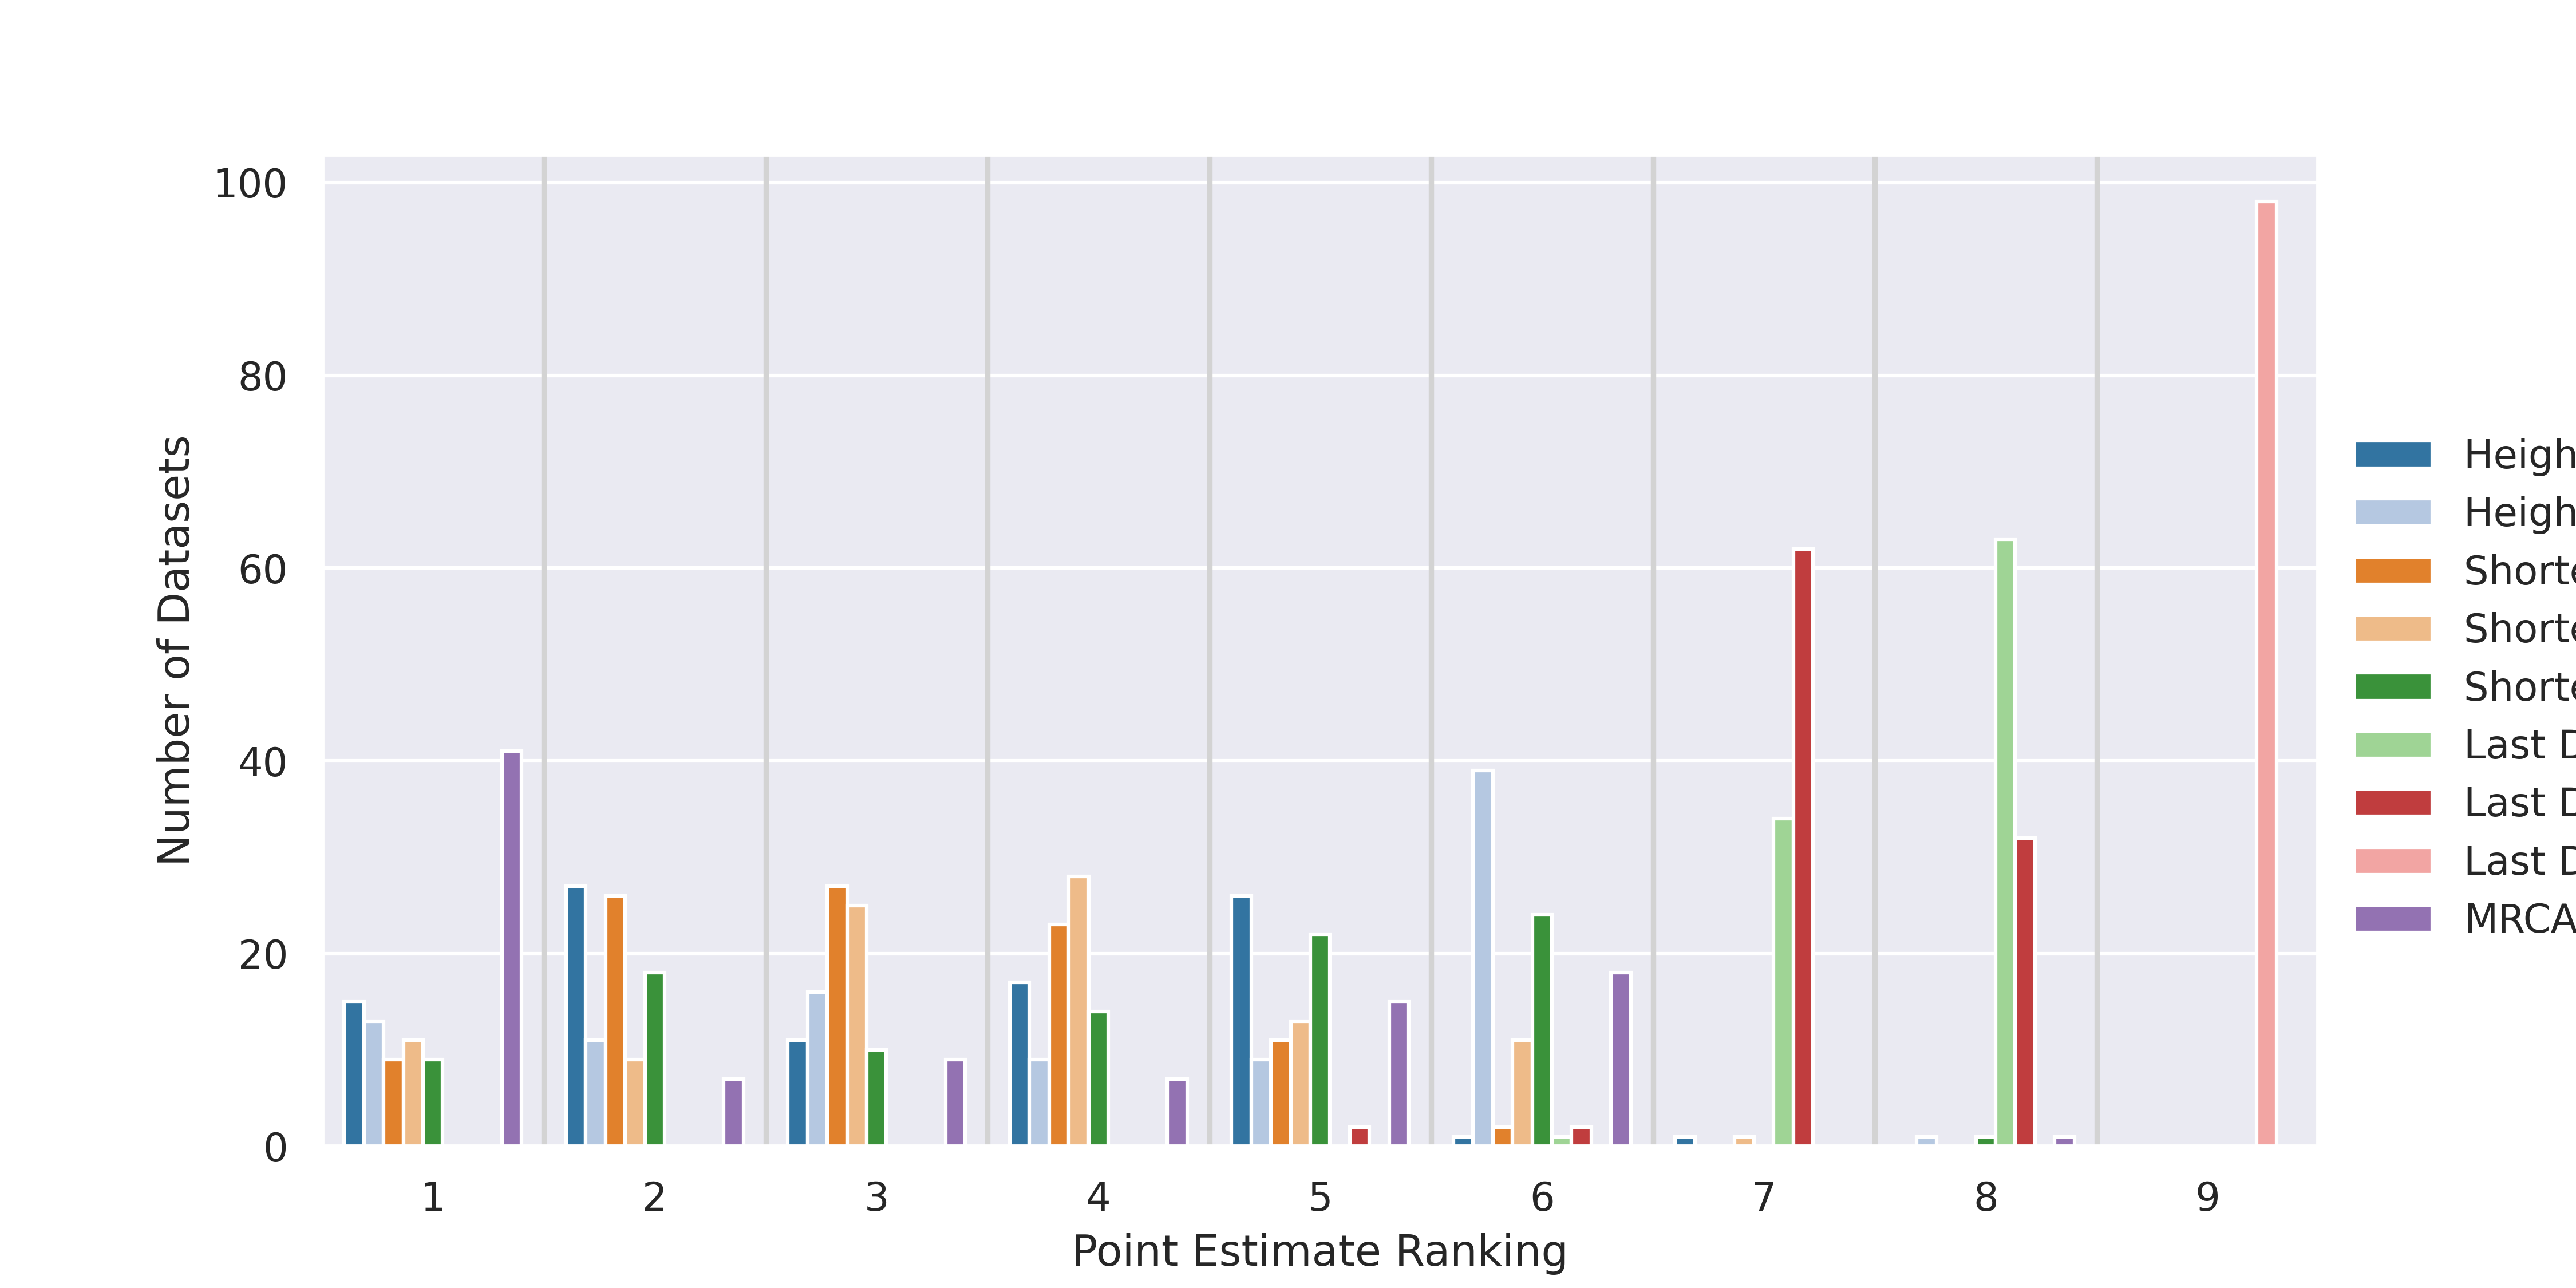
\includegraphics[width=\textwidth]{figures/yule-100-ccd1-point-estimates-ranking.png}
		\subcaption{Yule-100}
	\end{subfigure}
	\begin{subfigure}[b]{0.45\textwidth}
		\centering
		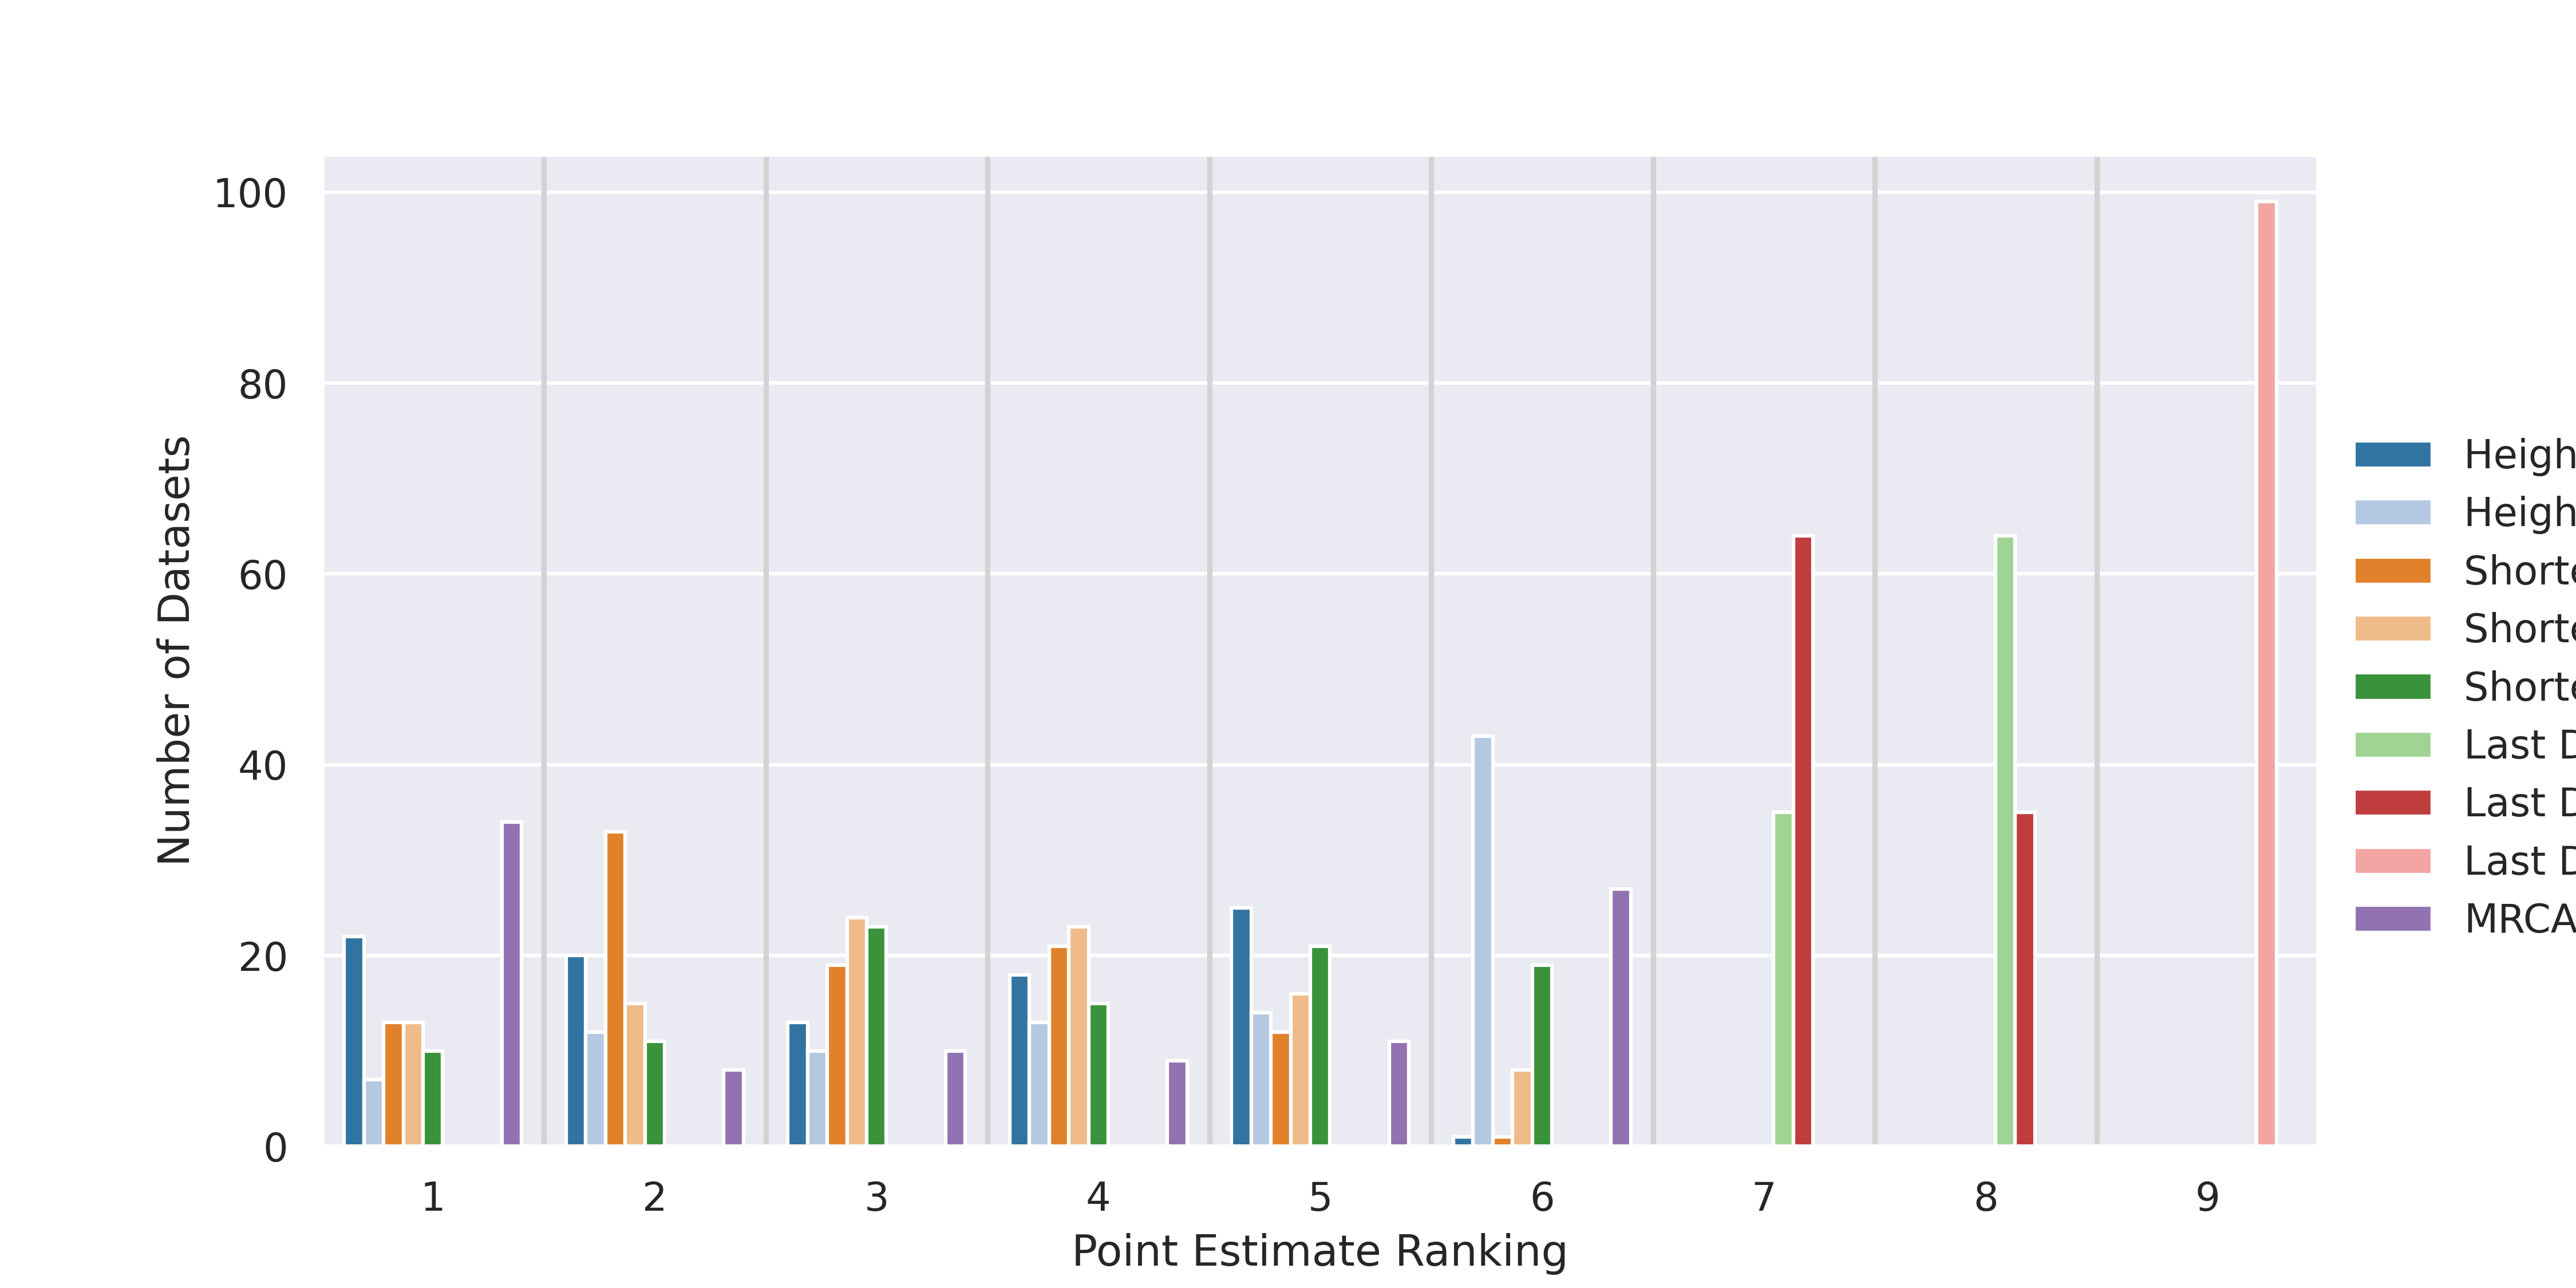
\includegraphics[width=\textwidth]{figures/yule-200-ccd1-point-estimates-ranking.png}
		\subcaption{Yule-200}
	\end{subfigure}
	
	\begin{subfigure}[b]{0.45\textwidth}
		\centering
		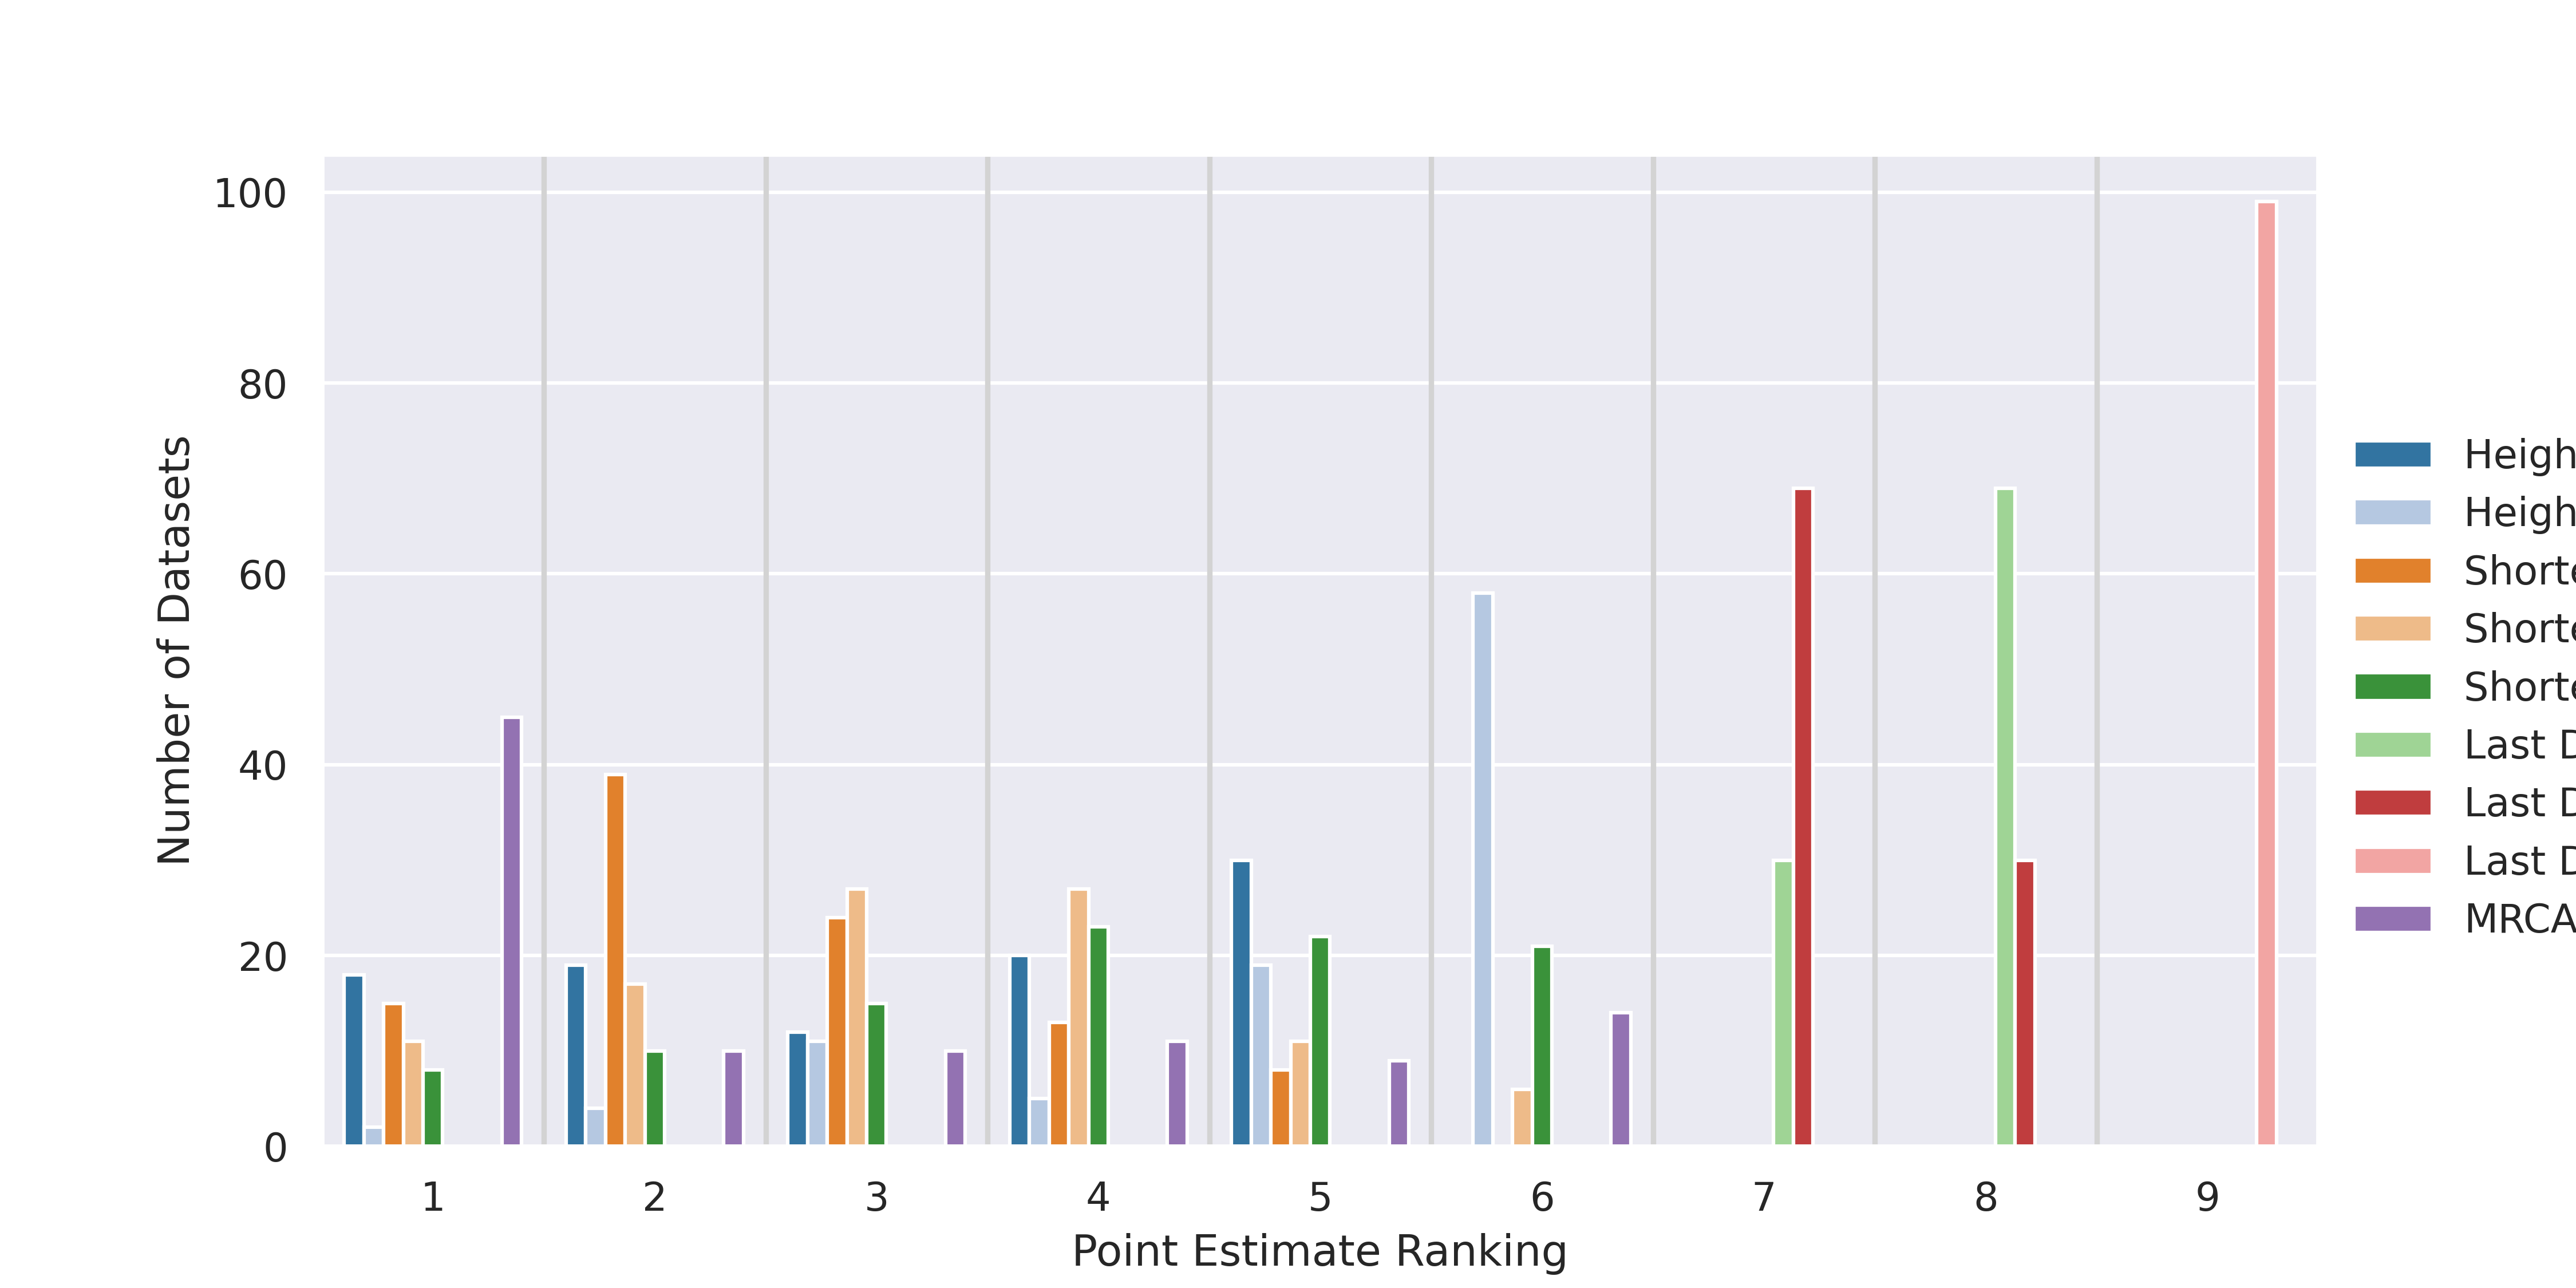
\includegraphics[width=\textwidth]{figures/yule-400-ccd1-point-estimates-ranking.png}
		\subcaption{Yule-400}
	\end{subfigure}
	
	\label{fig:accuracy-point-estimators-ranking}
\end{figure}

\section*{Discussion}

We have introduced a family of tractable time tree distributions designed to approximate posterior distributions based on MCMC samples. These distributions allow us to perform operations relevant to Bayesian phylogenetics research in an efficient manner. Going beyond point estimation, these distributions can be used to compare different evolutionary hypotheses, test if a tree is in the smallest 95\% credible region, or quantify the uncertainty of divergence times. All operations are accessible in a readily available software package \cite{juliapackage}. The package enables researchers to easily fit, select, and analyze these distributions using their own posterior samples.

Experiments with both simulated and real-world datasets show that, generally, the height ratio embedding using the beta distribution produces the highest joint data likelihood. Furthermore, it provides the best approximation of the credible regions for the real-world dataset and produces the best point estimates (although MRCA outperforms all distribution-based point estimators). The only shortcoming of the height ratio embedding is that it does not capture the credible regions of the simulated datasets as well as the alternatives. (Why is that?). The results for the shortest branch embeddings are comparable with those of the height ratio embedding regarding the joint data likelihood and the accuracy of the point estimates. Furthermore, they outperform the other embeddings in capturing the smallest credible regions on the simulated datasets. Distributions based on the last divergence embedding generally fall short in terms of the joint data likelihood and the accuracy of the point estimates. They perform similarly to the shortest branch embedding regarding the smallest credible regions.

Because of these mixed results, we advocate for a model selection approach. Researchers can employ likelihood-based model selection to determine the most suitable distribution for their specific dataset. In a second step, credible-region plots can be used to assess whether the credible sets are well-captured and if the approximate distribution can reliably be used to gain insight into the posterior distribution. This workflow is facilitated by the software package using a single bash command. In case only a point estimate is needed, the results suggest resorting to the default method implemented in TreeAnnotator \cite{treeannotator}, as MRCA still outperforms the distribution-based point estimators.

While we focused on ultrametric trees, the approach can be further extended to non-ultrametric trees. One possibility is to design an additional (invertible) embedding step transforming a non-ultrametric tree into an ultrametric tree, and then use the introduced embeddings on the ultrametric tree.

All discussed distributions are based on basic embedding transformations, on well-known univariate distributions, and assume independence in the embedding space. While these choices offer simplicity and tractability, more sophisticated approaches might be better at capturing intricate dependencies within the vertex heights. One such approach is to leverage neural networks to learn embeddings directly from data. In particular, normalizing flows \cite{normalizingflow} and graph neural networks \cite{graphnn} have proven effective in the context of Bayesian subsplit networks \cite{subsplitnf,artree}.

We focus on modeling distributions on a clade level. Another promising approach is to model the distances between taxa, corresponding to their evolutionary distance. Several different tree spaces around this concept have been proposed, including the wald space \cite{wald}, the palm tree space \cite{tropical}, and the cube space \cite{cube}. However, the geometry of these spaces introduce significant challenges, particularly regarding the normalization of the probability density and sampling. Things get slightly easier if one drops the requirement of calculating the unnormalized posterior. One exciting possibility is to define a probability measure based on the distance metric defined in these spaces. Given the distance metric $d(T_1, T_2)$, a possible probability density could be inspired by the normal distribution and resemble $p(T) \sim \exp(d(T, \hat{T}) / \sigma^2)$ with the Fréchet mean $\hat{T}$ \cite{frechetmeanvar}. Given that the Wald space is equipped with a geometry of globally nonpositive curvature, the maximum likelihood estimators in that space are well-defined \cite{gaussianriemann} (but not necessarily tractable). Another benefit of a potential distance-based approache would be that they jointly model topology and branch lengths instead of treating them independently.

Finally, we defined our time tree distributions in the context of approximating the posterior as given by MCMC. However, another possible application is to use them for direct variational inference. The simplicity of these distributions makes them well-suited for this purpose, as their tractability allows for an effective variational approximation.

\section*{Conclusion}

This paper introduced tractable time tree distributions for summarizing MCMC posterior samples in Bayesian phylogenetics, enabling analyses beyond point estimates. We compared different embeddings and distributions on simulated and real-world datasets, finding that height ratio embeddings with beta distributions generally outperformed the alternatives. Because the results are dataset-dependent, we recommend model selection for optimal distribution choice. The accompanying software package facilitates researchers to fit and analyze these distributions using their own posterior samples. Future work could explore neural network embeddings and distance-based tree space approaches.

\section*{Supporting information}

\subsection*{Software package}

A software package written in Julia \cite{juliapackage} was developed implementing all the methods presented in this paper. It can be found at \url{https://github.com/tochsner/TractableTimeTreeDistributions} and can be used to fit and analyze the distributions for any time tree sample. A web version accessible from a browser is in development.

\subsection*{The curse of dimensionality}

This section examines the susceptibility of time trees to the \emph{curse of dimensionality} \cite{curse,curse2}, a phenomenon where the complexity of a problem increases exponentially with the number of dimensions. Specifically, we look at the pairwise Robinson–Foulds (RF) distances between the MCMC trees of the synthetic Yule datasets. We find that the distances increase with the number of taxa while the relative variation of the distances decreases (see figures \ref{fig:curse1} and \ref{fig:curse2}). This defies the intuition that regions of higher probability density should yield samples with closer proximity and might complicate the application of conventional distance-based methods to analyze the posterior sample. Previous work suggests that the curse of dimensionality might not be limited to simulated trees. The datasets analyzed by \cite{dimensionality} show a median intrinsic dimensionality of around $7$ when using the RF distance---potentially high enough to degrade the performance of distance-based methods \cite{curseimplications}.

\begin{figure}[H]
    \centering
    \begin{minipage}[t]{0.45\textwidth}
        \caption{The average pairwise Robinson–Foulds distance between the MCMC trees of the synthetic Yule datasets. The distances increase with the number of taxa.}
        
		\centering
        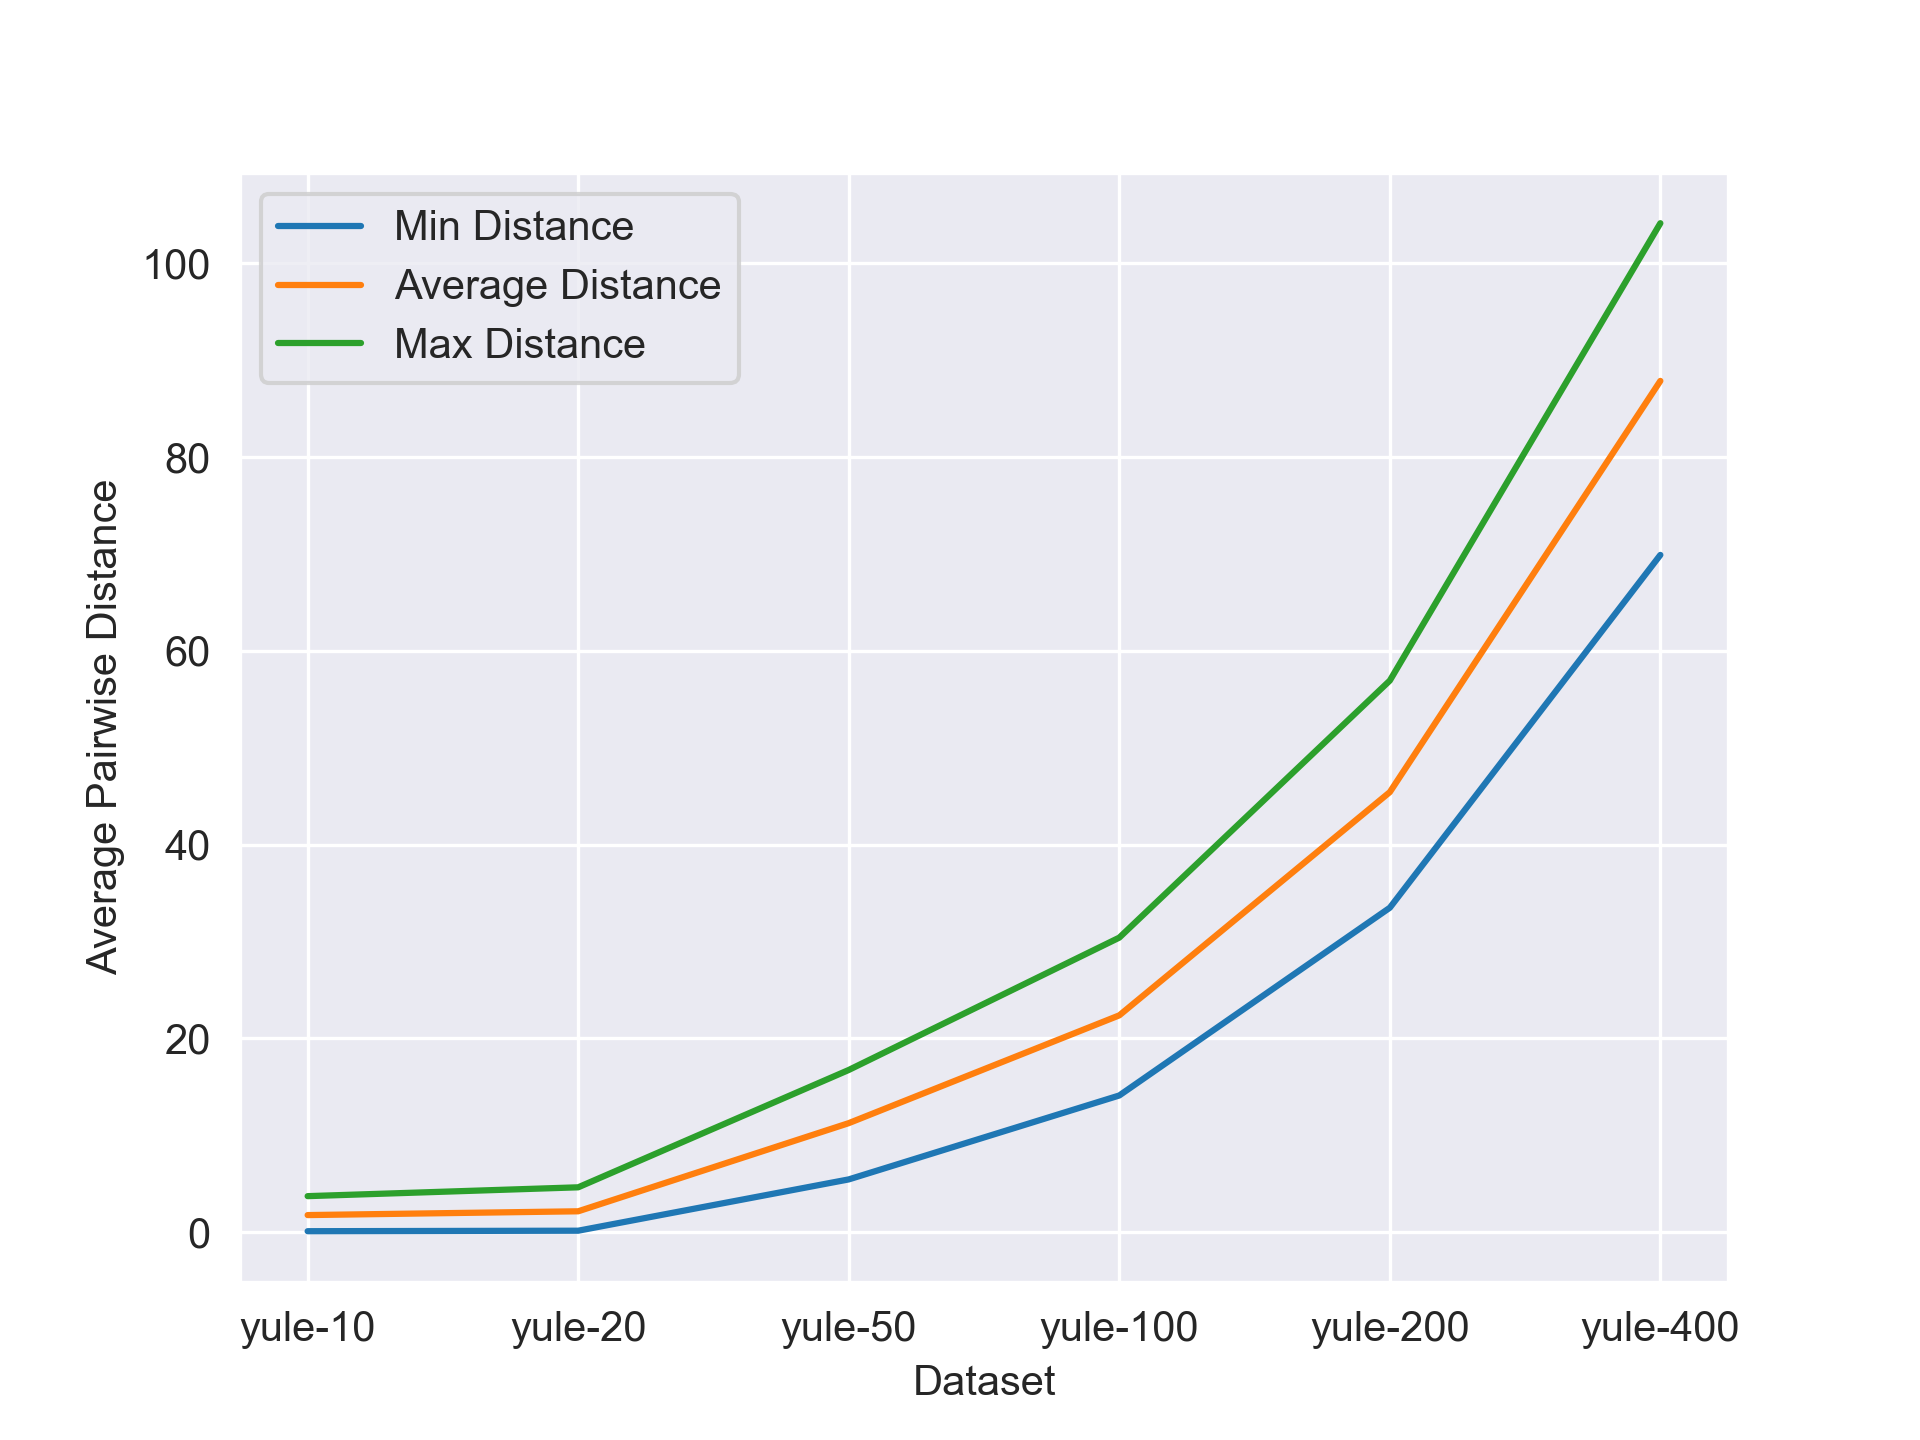
\includegraphics[width=\textwidth]{figures/curse_distance.png}

		\label{fig:curse1}
    \end{minipage}
    \hfill
    \begin{minipage}[t]{0.45\textwidth}
        \caption{The average ratio of the minimum to maximum pairwise Robinson–Foulds distance between the MCMC trees of the synthetic Yule datasets. The ratios decrease with the number of taxa.}
        
		\centering
        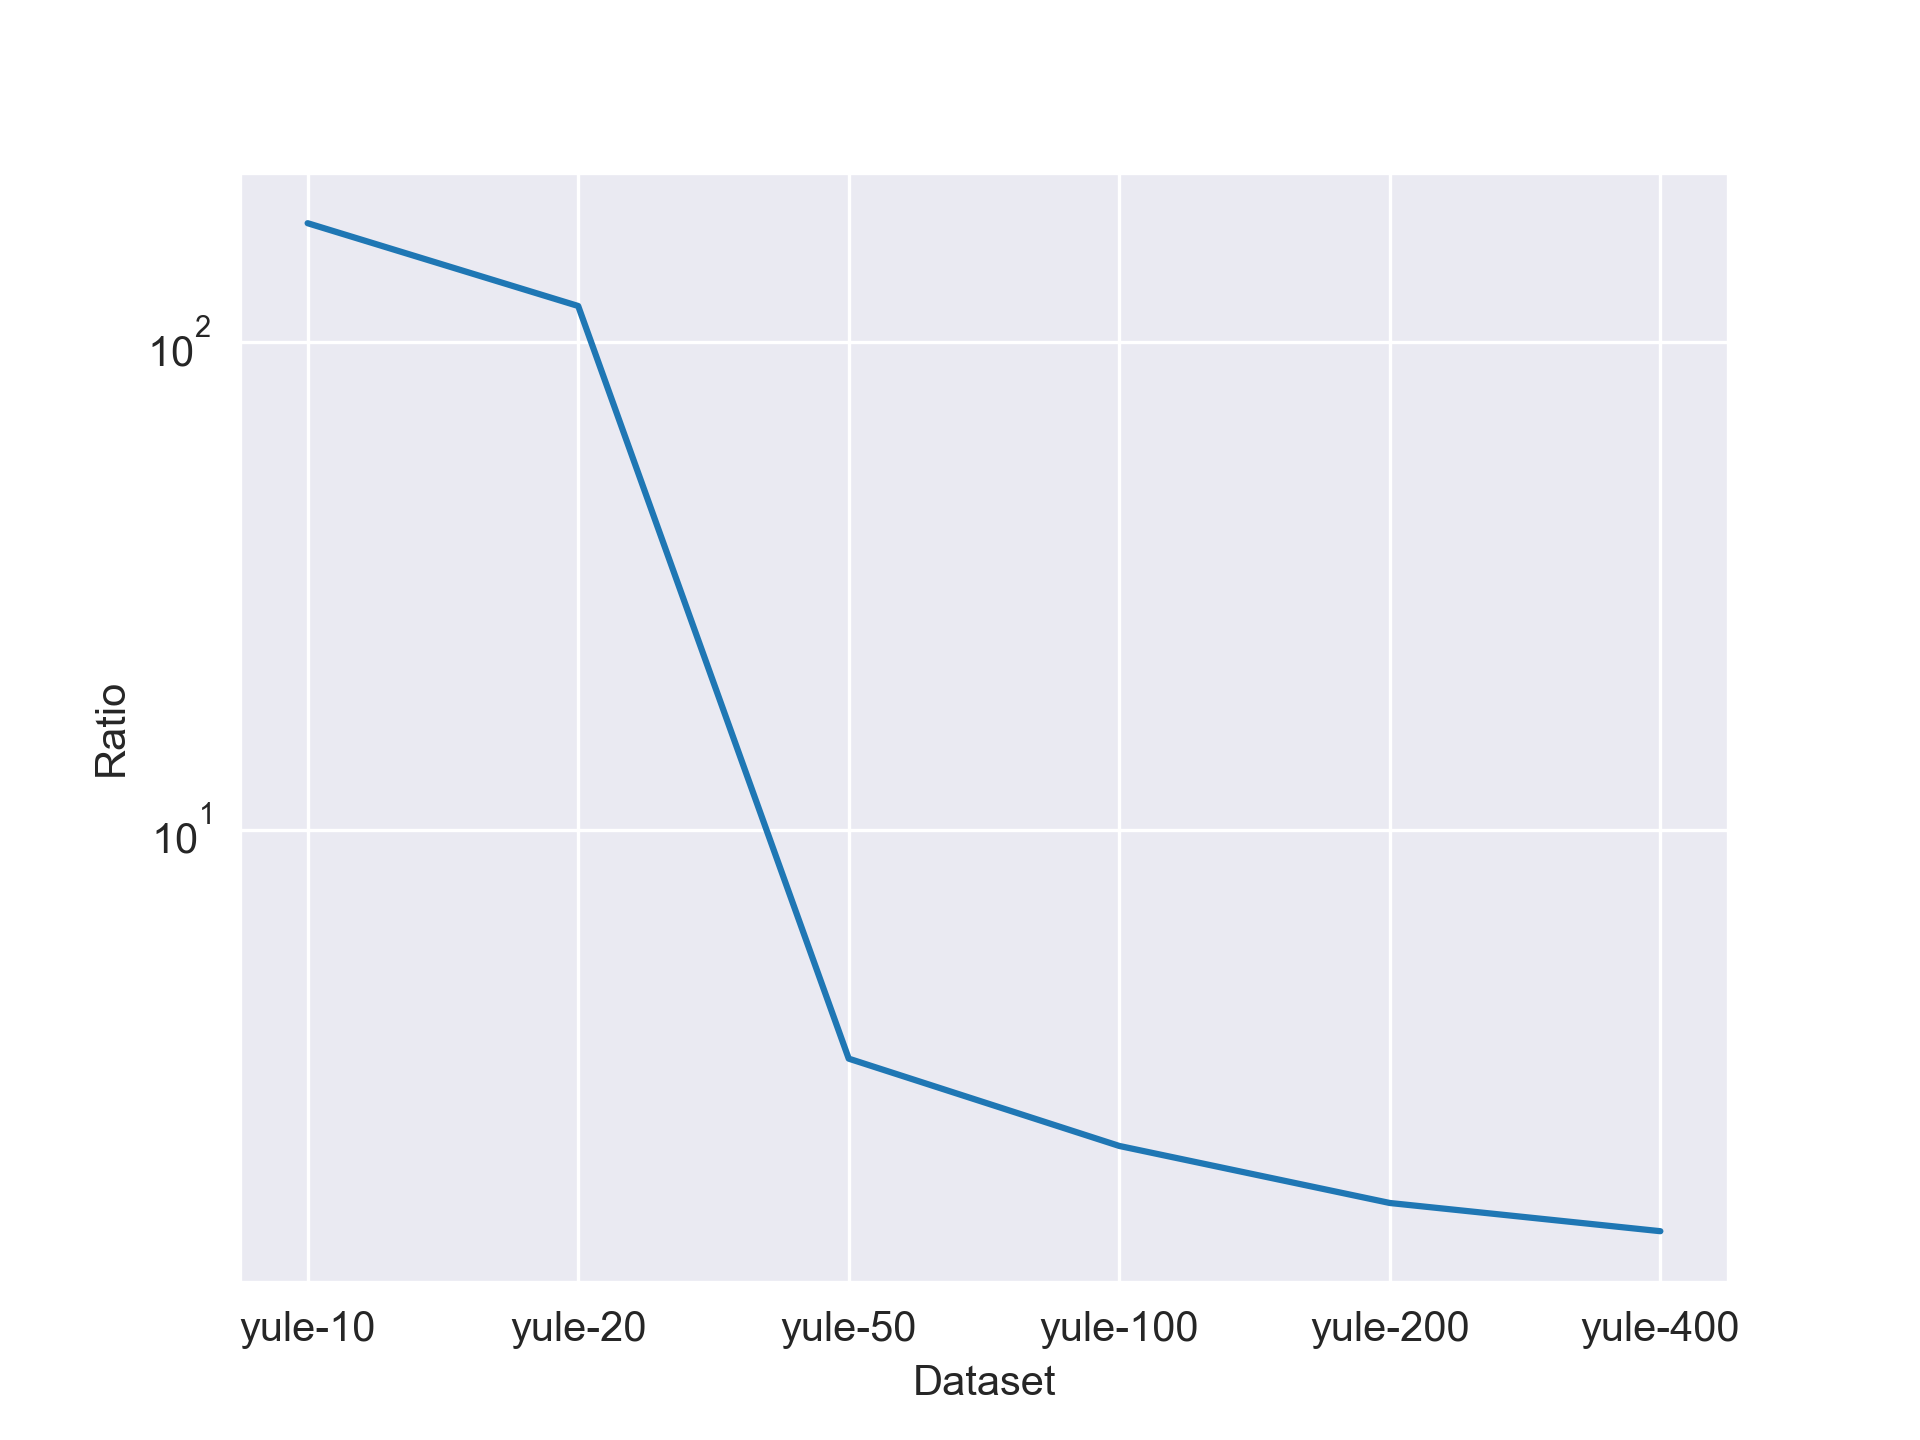
\includegraphics[width=\textwidth]{figures/curse_ratio.png}

		\label{fig:curse2}
    \end{minipage}
\end{figure}

\subsection*{Correlations}

% TODO

TODO

\subsection*{Tree ESS}

MCMC generates posterior time tree samples by performing a walk through the tree space, where new tree candidates are proposed by modifying the current tree using specific operations. Each tree depends on the previous one, resulting in autocorrelation in the samples. The maximum likelihood estimation and the data likelihood calculation assume that the samples are independently sampled. Thus, we estimate the effective sample size (ESS) of the MCMC samples and use it to subsample the posterior samples down to a set of (approximately) independent samples.

We use two methods to estimate the tree ESS. Both methods work by transforming each tree into a continuous parameter and assessing the effective sample size of the resulting set of continuous parameters (trace) \cite{treeess,vehtari2021rank}. The first trace consists of the sum of the branch lengths for each tree. The second trace corresponds to the Robinson-Foulds distance to the CCD1-MAP tree \cite{ccd}. We then use the smaller ESS of these two traces to estimate the ESS of the posterior tree samples.

\subsection*{Simulated datasets}

The following LinguaPhylo \cite{linguaphylo} script was used to generate the simulated datasets. Only the number of taxa (n) was changed for the different runs.

\begin{lstlisting}[basicstyle=\small]
data {
	L = 300;
	clockRate = 1.0;
	nCatGamma = 4;
	birthRate = 25.0;
	n = 100;
}
model {
	frequencies ~ Dirichlet(conc=[5.0, 5.0, 5.0, 5.0]);
	kappa ~ LogNormal(meanlog=1.0, sdlog=1.25);
	Q = hky(kappa=kappa, freq=frequencies);
	shape ~ LogNormal(meanlog=-1.0, sdlog=0.5);
	siteRates ~ DiscretizeGamma(
		shape=shape, ncat=nCatGamma, replicates=L
	);
	phi ~ Yule(lambda=birthRate, n=n);
	D ~ PhyloCTMC(
		L=L, Q=Q, mu=clockRate,
		siteRates=siteRates, tree=phi
	);
}
\end{lstlisting}

\subsection*{Real-world datasets}

We refer to the Excel file in the supporting information for a list of studies considered and possible reasons for exclusion of a dataset. All datasets can be downloaded from the Dryad repository \cite{dryad} and the curated \emph{Phylogenetic Posterior Tree Datasets} repository \cite{tree_dataset} found at \url{https://github.com/tochsner/phylogenetic-tree-posterior-datasets}.

\nolinenumbers

\bibliography{refs}

\end{document}

